\chapter{Pattern Recognition and Implementation}

% **************************** Define Graphics Path **************************

\epstopdfsetup{outdir=Chapter4/Figs/PDF/}
\ifpdf
    \graphicspath{{Chapter4/Figs/Raster/}{Chapter4/Figs/PDF/}{Chapter4/Figs/}}
\else
    \graphicspath{{Chapter4/Figs/Vector/}{Chapter4/Figs/}}
\fi


\section{Implementing the Color Space}\label{sec:ImplementingTheColorSpace}

In the previous two chapters, we have been approaching the color space design problem mathematically. Here, we will outline the practical implementation of the color space algorithm on the mobile device.

The first and most pressing consideration is limited processing power; while our mathematical approach to the algorithm design is significantly faster and more efficient than the more typical color space algorithms --- as will be discussed in the following chapter --- minimizing the number of clock cycles spent on continuous processes is necessary in order to ensure efficient operation. In the case of redistribution, the integer matrix transform is performed first, which puts the pixel values in the quantized working type $qRsRange$ described in Chapter 2, then pixel classification is performed before any of the chromatic information is redistributed as illustrated in Figure \ref{fig:PartitioningRegions}.

The pixel classification is performed before the redistribution because it excludes processing pixels which are of no interest based on both chromatic channels, whereas for redistribution one channel may clearly lie outside of the discard region $\lambda$ while the other could be kept or redistributed. With the pixel classifier, if one channel lies outside the discard region, the other is also of no interest since the pixel value is outside of the partitioning region, thereby avoiding unnecessary processing time spent on redistribution. The classification is straightforward within the limits on the channel values, so it isn't sophisticated like an elliptical partitioning or a probabilistic Gaussian-based thresholding; it is simply a quick way of excluding the majority of the pixel values which aren't of interest.

Once the pixels have been classified, the redistribution is performed --- which requires further processing --- or we assign a pixel value from a small set of possibilities and skip onto the next pixel value. The redistribution function is applied to the working type $tRange$, while the comparison and classification is done in $qRsRange$. This is because the information in $tRange$ is compressed to avoid wasting space, and as a consequence of this it does not occupy the full data type. $qRsRange$, on the other hand, being the natural range multiplied by the quantization matrix qR, does occupy the full data type. Since the operation is simply a comparison between numbers, it is of no advantage to compress the information so tightly. Additionally, since $qRsRange$ is a signed range, one could look at the bit indicating the sign and immediately tell whether or not a given value will be discarded. Once scaled to $tRange$, the redistribution function is applied --- which has a source range of $tRange$ and a range $dRange$ of the destination type --- as outlined in Section \ref{sec:PreservationOfColorInformation} in Chapter 2.

It should be noted that the region between the extended keep region $\omega p$ and the discard region $\lambda$ is not especially large; for even a $5\sigma$ result, it's only tens of values wide. As such, we use a lookup table for the redistribution in our actual implementation, thus further reducing the processing overhead. The C++ implementation has a lookup table threshold set to 64, a quarter of the source data type range. If the redistribution region is larger than that, the error function approximation from Chapter 2 is used. This is mainly for future-proofing the implementation; given the limited size of the region, we fully expect to use a lookup table for all practical cases.

As another future concession, the facility to add pixel-based functions to the color space transform, such as the skin probability function mentioned at the end of the previous chapter, is allowed. The color space transform is a threaded process, so there is no way of knowing that the last pixel value that was processed by any given thread was an adjacent pixel, as the parallelization is handled by OpenCV's universal threading library implementations. Pixel-based functions, however, are per-pixel processes, and they come out as separate resulting channels, so they can be added to the color space transform without causing any conflicts.



\subsection{The White-Out Black-Out Algorithm}\label{sec:WhiteOutBlackOutAlgorithm}
We need to find the point at which a chromatic value begins to suffer from white-out and black-out. This is done by taking the corresponding RGB value for the chromatic point and illuminating and deluminating the point by shifting the channel values by the same amount, noting when each channel value becomes fully saturated or desaturated. This is done in the unit space so the results can be scaled to any working range. The algorithm for finding the theoretical values is given in Algorithm \ref{algo:TheWhiteoutBlackoutAlgorithm} below. 

\begin{algorithm}[H]
 \begin{algorithmic}
  \Require{ $Ca$, $Cb$ The chromatic values}
  \State \phantom{Require}  { $iLCaCb$ the transform to LCaCb from RGB; }
  \State \phantom{Require}  {  $LCaCb$ the transform to RGB from LCaCb}
 \Ensure{  The luminosity at which black out $L_{BO}$  and white out $L_{WO}$ occur.}
 \State \phantom{Ensu} { \begin{tabular}{l}
 $Ca_{min}  \le Ca \le Ca_{max}$   \\ 
 $Cb_{min}  \le Cb \le Cb_{max}$  
 \end{tabular}  \parbox{0.65 \textwidth}{The chromatic range which could be suffering from white-out or black-out}}
 
   \State  $pnt^{RGB} \gets iLCaCb(0.5, Ca,Cb)$ \Comment{Put the point in RGB space }
   \State  $O \gets Order(pnt^{RGB}, \#1> \#2)$ \Comment{The order of the RGB channels from largest to smallest}
   \State  $\Delta WO_1 \gets 1 - pnt^{RGB}_{O(1)} $ \Comment{Iluminate to make the largest channel value saturated}
   \State  \phantom{Set} $pnt^{(RGB, WO, 1)}_{O(1)} \gets 1 $ \Comment{The point where a channel is saturated }
   \State  \phantom{Set} $pnt^{(RGB, WO, 1)}_{O(2)} \gets  pnt^{RGB} _{O(2)} + \Delta WO_1 $ 
   \State  \phantom{Set} $pnt^{(RGB, WO, 1)}_{O(3)} \gets  pnt^{RGB} _{O(3)} + \Delta WO_1 $ 
   \State  $\Delta WO_2 \gets 1 - pnt^{RGB}_{O(2)} $\Comment{Iluminate to make the second largest channel value saturated}
   \State  \phantom{Set}$pnt^{(RGB, WO, 2)}_{O(1)} \gets 1 $ \Comment{The point where two channels are saturated }
   \State  \phantom{Set}$pnt^{(RGB, WO, 2)}_{O(2)} \gets 1 $ 
   \State  \phantom{Set}$pnt^{(RGB, WO, 2)}_{O(3)} \gets  pnt^{RGB} _{O(3)} + \Delta WO_2 $ 
     
     
   \State  $\Delta BO_1 \gets  pnt^{RGB}_{O(3)} $ \Comment{Deluminate by the smallest channel value}
   \State  \phantom{Set}$pnt^{(RGB, BO, 1)}_{O(1)} \gets  pnt^{RGB} _{O(1)} - \Delta BO_1  $ \Comment{The point where a channel is desaturated }
   \State \phantom{Set} $pnt^{(RGB, BO, 1)}_{O(2)} \gets  pnt^{RGB} _{O(2)} - \Delta BO_1 $ 
   \State \phantom{Set} $pnt^{(RGB, BO, 1)}_{O(3)} \gets  0 $ 
   \State  $\Delta BO_2 \gets pnt^{RGB}_{O(2)} $ \Comment{Deluminate by the second smallest channel value}
   \State  \phantom{Set} $pnt^{(RGB, BO, 2)}_{O(1)} \gets pnt^{RGB} _{O(1)} - \Delta BO_2 $ \Comment{The point where two channels are desaturated }
   \State  \phantom{Set} $pnt^{(RGB, BO, 2)}_{O(2)} \gets 0 $ 
   \State  \phantom{Set} $pnt^{(RGB, BO, 2)}_{O(3)} \gets 0 $ 
     
   \State  $pnt^{(WO, i)}\gets LCaCb(pnt^{(WO, i)}) $ \Comment{The white-out points in LCaCb color space}
   \State  $pnt^{(BO, i)}\gets LCaCb(pnt^{(BO, i)}) $ \Comment{The black-out points in LCaCb color space}
   
   \State  $L_{WO} \gets pnt^{(WO, 1)}_1$ 
   \State  $L_{BO} \gets pnt^{(BO, 1)}_1$ 
   \State  $Ca_{min}  \gets Min(pnt^{(WO, 1)}_2, pnt^{(WO, 2)}_2, pnt^{(BO, 1)}_2, pnt^{(BO, 2)}_2 )$ 
   \State  $Ca_{max} \gets Max(pnt^{(WO, 1)}_2, pnt^{(WO, 2)}_2, pnt^{(BO, 1)}_2, pnt^{(BO, 2)}_2 )$ 
   \State  $Cb_{min}  \gets Min(pnt^{(WO, 1)}_3, pnt^{(WO, 2)}_3, pnt^{(BO, 1)}_3, pnt^{(BO, 2)}_3 )$ 
   \State  $Cb_{max} \gets Max(pnt^{(WO, 1)}_3, pnt^{(WO, 2)}_3, pnt^{(BO, 1)}_3, pnt^{(BO, 2)}_3 )$ 
     
  \State \textbf{Return} {$L_{WO} , L_{BO} , Ca_{min}, Ca_{max} , Cb_{min}, Cb_{max}$ }
 
  \end{algorithmic}
    \caption{The White-Out Black-Out Algorithm}
    \label{algo:TheWhiteoutBlackoutAlgorithm}
 \end{algorithm}
 
 The theoretical values are adjusted by 10\% to account for the auto brightness and contrast adjustment performed by the phone as described in Section \ref{sec:WhiteoutAndBlackout}. We only wish to adjust the bounds away from the luminosity axis. One of the chromatic bounds will be the luminosity axis $Ca=\frac{1}{2}$ or  $Cb=\frac{1}{2}$, as this is the white or black point. Whether the bound is the upper or lower limit depends on the starting point, so we define a function which performs the adjustment appropriately.
 
 \begin{equation}
 slack(x) = \begin{cases}
 (1-a) x     & x < \frac{1}{2} \\
 (1+a) x     & x > \frac{1}{2} \\
 \frac{1}{2} & x = \frac{1}{2} 
 \end{cases} \quad \text{where} \quad a = 0.1
   \end{equation}
 We can now write the condition for whether a value could have suffered from white-out or black-out. 
  \begin{multline}\label{eq:InWoBoRegion}
 (( 0 \le L \le  slack(L_{BO}) ) \vee ( slack(L_{WO}) \le L \le 1) ) \wedge  \\
 slack(Ca_{min}) \le Ca \le  slack(Ca_{max}) \wedge  \\
 slack(Cb_{min}) \le Cb \le  slack(Cb_{max})
  \end{multline}
  
  \subsection{The Region Classification and Partitioning Function}\label{sec:TheRegionClassificationAndPartitioningFunction}
  It is desirable to classify a pixel value after rotation but before redistribution in-order to avoid unnecessary work on pixel values which are not of interest. This can be done to a degree, but it is necessary to assume reasonably uniform lighting conditions or by using boundaries set by the WOBO algorithm above \ref{sec:WhiteOutBlackOutAlgorithm}. The pixel values are classified by chromatic value as either inside the target region or outside in each chromatic axes, dividing the chromatic plane into nine regions, as illustrated in Figure \ref{fig:PartitioningRegions}. A rudimentary partitioning is performed by assigning 8 constant chromatic vectors to the values outside the target region around the mean. The chromatic channel values are not evaluated further for values outside the target region. The luminosity is always evaluated, because all that is required is a scaling from $qRsRange$ to the destination range $dRange$  and the luminosity is needed to choose appropriate bounds using the WOBO algorithm.
  
  \begin{figure}[h!]
    \centering
      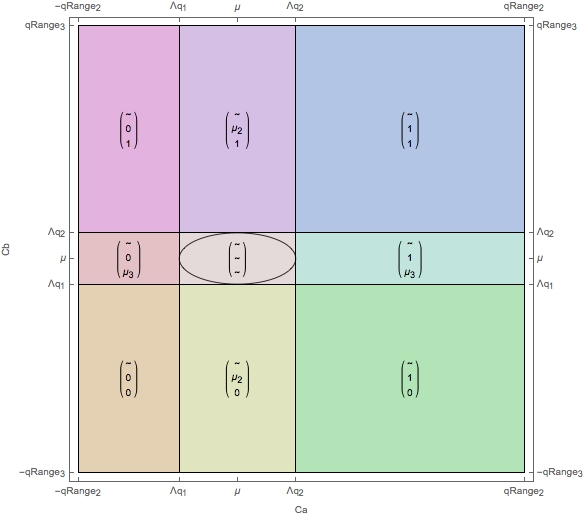
\includegraphics[width=0.80\textwidth]{Chapter4/Figs/PartitioningRegion.jpg}
      \caption{The Regions in the chromatic space. A $ \sim $ indicates values which will undergo redistribution. Regions outside the target area are allocated extreme values at the edge of the color space}  \label{fig:PartitioningRegions}
  \end{figure}
  
  
  
  \subsection{Floating the Mean}\label{sec:FloatingTheMean}
  Different lighting conditions can affect the detected pixel color. Not accounting for strongly-colored light, the affect of different lighting conditions is to increase or decrease the saturation of the color. The distribution is relatively unaffected in orientation or variance, meaning that lighting conditions can be accounted for by adjusting the mean. 
  \newcommand{\newMean}{\widetilde{\mu}}
  The algorithm adjusts to ambient lighting by first taking a reference image centered on a patch of skin and finding the mean in the LCaCb color space. This new mean $\newMean$ is then used in the current instance of the algorithm. It is adventitious to keep the mean adjustable in the routine, so this is implemented by introducing an adjustment parameter $\delta\mu$ to the routine, where $\newMean = \mu + \delta\mu$. The algorithm assumes that the adjustment is small enough that the distribution function retains the same shape aside from a translation along the axis. This allows the distribution parameters to be adjusted by simply shifting them by $\delta\mu$. 
  
  \begin{equation}
  \begin{aligned}
   \widetilde{\lambda}_1 & = \lambda_1 + \delta\mu &  \widetilde{\lambda}_2 & = \lambda_2 + \delta\mu \\
   \widetilde{\omega}_1 & = \omega_1 + \delta\mu &  \widetilde{\omega}_2 & = \omega_2 + \delta\mu 
  \end{aligned} \quad \text{Where} \quad \lambda_1 < \delta\mu < 1 - \lambda_2
  \end{equation}
  
  \subsection{Loosened Deviation}\label{sec:LoosenedDeviation}
  
 \afterpage{ \begin{figure}[h!]
    \centering
      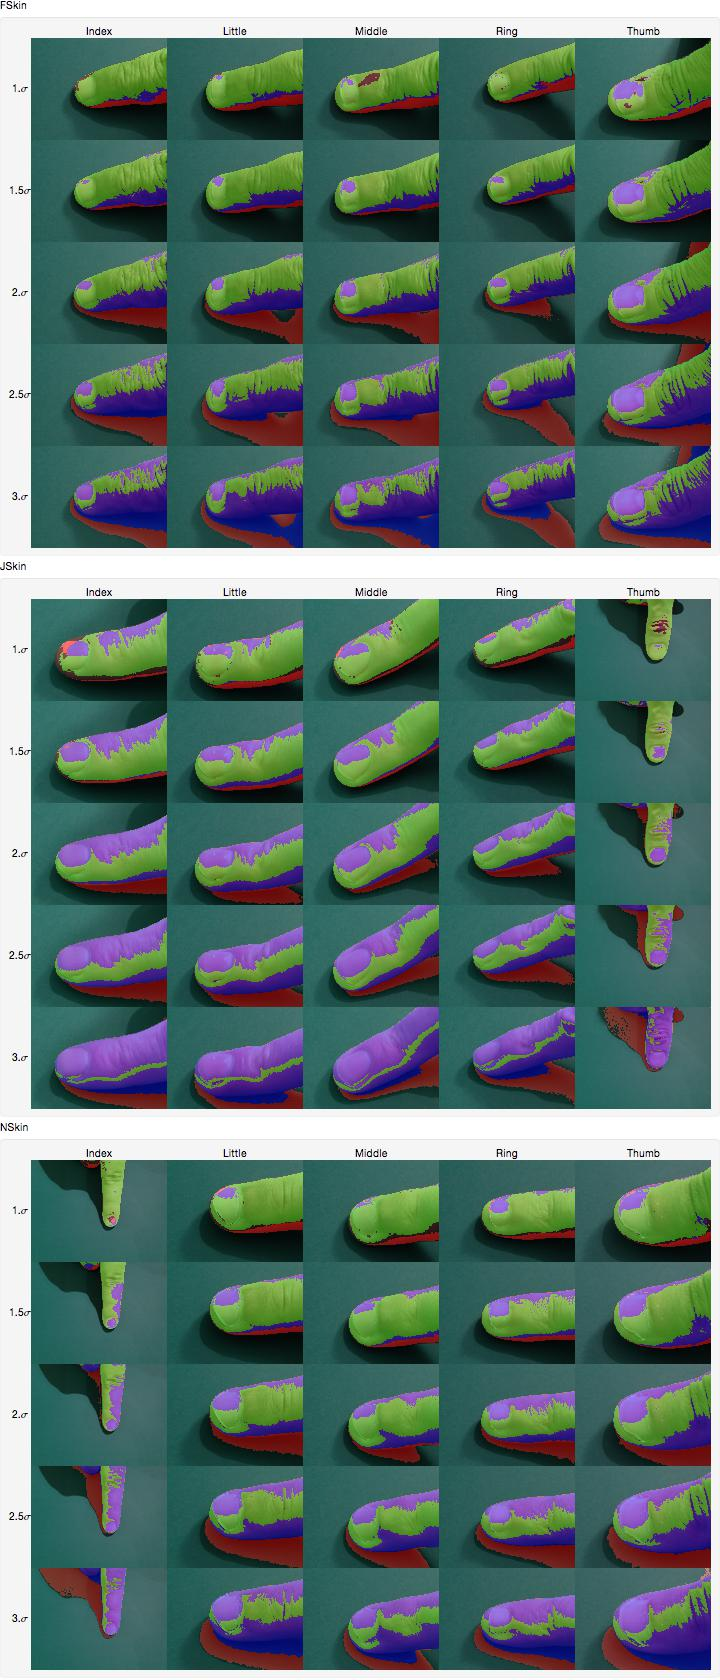
\includegraphics[width=0.85\textwidth,height = \textheight]{Chapter4/Figs/RelaxingSigma.jpg}
      \caption{A selection of images classified using the quaternary method outlined in section \ref{sec:QuaternaryPixelClassification}, with various values of $\sigma$. It can be seen that $1\sigma$ correctly classifies the majority of pixels, however it classifies some on-digit pixels as "probably not skin", and even "not skin". $3\sigma$, meanwhile, includes large portions of shadow as "probably skin". A compromise of $2\sigma$-$2.5\sigma$ is therefore suggested.} \label{fig:RelaxedSigma}
  \end{figure}
  \clearpage
  }
  
  The standard deviation found in Chapter 3 is a very tight fit to the chromatic values taken under controlled lighting conditions. For our practical implementation, this tight fit needs to be relaxed. This is done empirically by trying out multipliers of the standard deviation $\sigma$ on the image sets. What is desired is a multiplier which relaxes the redistribution such that all the pixel values on a given digit are classified as skin, and all the background is classified as not skin. This is done empirically using the quaternary classification presented in Section \ref{sec:QuaternaryPixelClassification} below, which accounts for white-out and black-out and classifies the pixel value as "definitely skin", "probably skin", "probably not skin", and "not skin".
  
  Using a value of 2.3 times the original $\sigma$ correctly classifies the pixel values; this was found by observing tables of images similar to those in Figure \ref{fig:RelaxedSigma}. 
  
  
  \subsection{The Color Space Algorithm as Implemented}\label{sec:ColorSpaceAlgorithmAsImplemented}
  Here we present the color space algorithm in a way which most closely resembles the C++ code. The construction of the color space object is described at the end of Chapter 2; here, the operation of the algorithm is described.
  
  First, we determine the form of the distribution function for a working type $tRange$ with the source range $srcRange=2^n$  and destination range $dstRange=2^m$ expressed in terms of their bit depths.
  
  \begin{gather*}
  \begin{aligned}
  K & =  2^{m-n}  \quad & \quad  
  \tRange(\theta,\mu,\sigma)   & =  \mathbf{l} \; 2^n \quad & \quad
  \mathbf{l}  & = \min\left\{ 2^{m-n}\delta(\mu,\sigma) \right. ,  \left. \mathbf{L}(\theta) \right\} 
   \end{aligned} \\
   \begin{aligned}
    \tMin(\theta,\mu,\sigma)   & =
   \begin{pmatrix}
      0 \\
    -\mathbf{l}_2 \; 2^{n-1}  \\  
    -\mathbf{l}_3 \; 2^{n-1} \\  
   \end{pmatrix} \quad & \quad
    \tMax(\theta,\mu,\sigma)   & =
   \begin{pmatrix}
    \mathbf{l}_1 \; 2^n  \\
    \mathbf{l}_2 \; 2^{n-1}  \\  
    \mathbf{l}_3 \; 2^{n-1} \\  
   \end{pmatrix} \quad & \quad
     \Scale &=
      \mathbf{l} \otimes
     \begin{pmatrix}
       \frac{1}{3} \\
      2^{1-n } \\
      2^{1-n }  \\
     \end{pmatrix}    \\
   \end{aligned}
  \end{gather*}
  
  Substituting into the distribution function \ref{eq:disFunction} gives us
  
  \begin{equation}
\textbf{dis}(x) =  -\frac{2^n \left(\text{erf}\left(\frac{2 \mu +1}{2 \sqrt{2} \sigma }\right)+\text{erf}\left(\frac{2^{1-2 n} x-\mu }{\sqrt{2} \sigma }\right)\right)}{\text{erf}\left(\frac{2 \mu -1}{2 \sqrt{2} \sigma }\right)-\text{erf}\left(\frac{2 \mu +1}{2 \sqrt{2} \sigma }\right)} \quad \textbf{where} \quad
\begin{array}{rl}
qMin < & x  < qMax \\
0 < &\mu <1\\
0 < &\sigma <1
\end{array}
  \end{equation}
  
  This form takes the result of the rotation directly, however we wish to add the flexibility to adjust the mean and use a lookup table for the values. It is desirable to keep the lookup table as short as possible. The maximum compression of the information without losing relevant information is given by compressing to $tRange$. The number of values in the lookup table can be reduced by scaling $x$ by a range $qtRange$, which is chosen to balance lookup table size and computational scaling efficiency.  Noting that $\mathbf{l} <2$, $qRsRange$ can be chosen to be equal to $tRange$ as if $\mathbf{l} =2$, which means that $qtRange$ is a power of two, allowing the scaling to be performed by bit shifting the value of $x_{qt} = x \ll n-2$. However, in the region where the function is applied, the information is preserved at best 2-to-1, so the information density can be reduced by half $x_{qt} = x \ll n-1$. Adjusting the mean changes the bounds on the region to be redistributed such that the form of the function does not change. For this reason, we also define $x$ relative to the bounds, which allows the same lookup table to be used regardless of any adjustment to the mean.
  
    \begin{equation}
  \textbf{dis}(x) =  \begin{cases}
    \textbf{disLU}((x-\Lambda_{1}) qtRange)  & \Lambda_{1} < x < \Omega_{pq1} \\
  \textbf{disLU}((x-\Omega_{pq2}) qtRange)  & \Omega_{pq2} < x < \Lambda_{q2} \\
  \textbf{dis}(x)  & \text{Otherwise}
    \end{cases} \quad \text{where} \quad 
    qtRange = \left(\begin{smallmatrix}
    \cdots \\ 2^{1-n}\\2^{1-n}
    \end{smallmatrix}\right)
    \end{equation}
  
  Aside from these refinements, the algorithm presented in Chapter 2 is used to perform the rotation and redistribution as described. The algorithm proceeds as follows:
  
  \begin{itemize}
  \item Interactively find an adjustment to the mean  $\delta\mu$.
  \item Set the new distribution parameters.
  \item Rotate the pixel value with the $\qR$ matrix: $ pxl_{q} = \qR \cdot pxl_{RGB}$ then $ \frac{- qRsRange}{2} < pxl_{q} < \frac{ qRsRange}{2}$
  \item Partition the rotated values to avoid unnecessary processing of irrelevant information.
  \item Apply any user supplied per-pixel functions to the rotated value and add as extra channels.
  \item Redistribute the rotated values into the destination type.
  \item Apply and user supplied per-pixel functions to the redistributed values.
  \end{itemize}

\section{Pattern Recognition Routines}\label{sec:PatternRecognitionRoutines}
In this section, pattern recognition routines which use the new color space are presented and discussed.

\subsection{Quaternary Pixel Classification}\label{sec:QuaternaryPixelClassification}

\newcommand{\WoBoBool}{\underset{\scalebox{0.5}{WoBo}}{\mathbb{L}}}
\newcommand{\ColorSquareBool}{\underset{ \scalebox{0.5}[0.5]{square} }{ \mathbb{C} } }
\newcommand{\ColorEllipseBool}{\underset{ \scalebox{0.5}[0.5]{ellipse} }{ \mathbb{C} } }

\begin{figure}[h!]
  \centering
    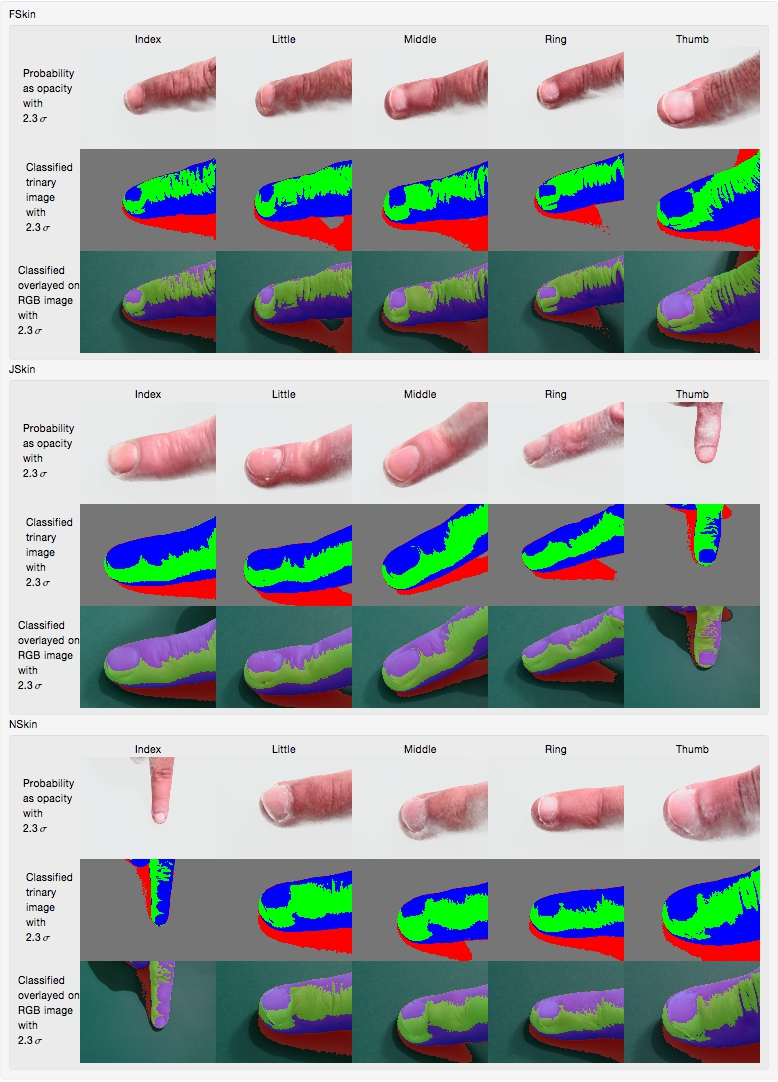
\includegraphics[width=0.95\textwidth]{Chapter4/Figs/ClassifiedSkin.jpg}
    \caption{The Quaternary Pixel Classification presented alongside the probability scored image for comparison.}\label{fig:2BitImage}
\end{figure}

We wish to classify the pixel values as either skin or not skin whist taking account of the reliability of the detected color due to whiteout and blackout effects. This is done by applying equation \ref{eq:InWoBoRegion} and setting a boolean flag $\WoBoBool$ accordingly. The square partitioning performed earlier in the algorithm also sets a boolean flag $\ColorSquareBool$ to 1 if the pixel is within the target range and to 0 otherwise. These can be combined to produce a 2-bit image which indicates both if the pixel value is in the target chromatic range and the reliability of the classification.
% 

\begin{center}
\begin{tabular}{|c|c|c|c|c|}
\hline
Correct                               & Unreliable      & \multicolumn{2}{|c|}{Image Bit} & \multicolumn{1}{|c|}{\multirow{2}{*}{Comment}}  \\ \cline{1-4}
Color $\ColorSquareBool$ & $\WoBoBool$ & $\ColorSquareBool$ & XOR($\ColorSquareBool$, $\WoBoBool$) & \\\hline
0 & 0 & 0 & 0 &  Definitely not the target \\\hline % & Wrong Color &    Reliable Luminosity 
0 & 1 & 0 & 1  & Possibly the target but shifted. \\\hline % & Wrong Color & Unreliable Luminosity
1 & 1 & 1 & 0  & \begin{tabular}{l} Probably the target but possibly \\ shifted into the target region \end{tabular} \\\hline % &   Right Color &    Reliable Luminosity
1 & 0 & 1 & 1  & Definitely the target \\\hline % &   Right Color & Unreliable Luminosity
\end{tabular}
\end{center}


This produces a 2-bit image. For this purpose, a 2-bit data type was added to OpenCV. The question then is how to use it. Essentially, we have four different states: values which are neither the right color nor in the right region; values which are possibly the right color, but because they're outside the valid region, they've potentially suffered from white-out and black-out; values which are in the right region, but the wrong color, and we are certain that they are not skin; and finally, values which are in the valid region and are of the right color. In the next subsections we will present some useful methods which take advantage of this quaternary classified image.

\clearpage
\subsection{The `Hurdle' Method}\label{sec:HurdleMethod}
The Hurdle method is an algorithm for finding a path inside an object using the quaternary classified image. The Hurdle method follows straight line paths in the object. As written, it is flexible enough to follow any straight line, however the current implementation takes a direction vector and evaluates at multiples of that direction vector. This means that non-horizontal and non-vertical lines are not guaranteed to be continuous. This is because the pixel values are not found using Bresenham's line algorithm. The algorithm has two thresholds --- a high and a low threshold. Whilst the pixel values remain in the high threshold, the path end point variable is updated; when the pixel values are in the lower threshold, the algorithm continues along the path, but without updating the path end point. This allows the path to pass through artifacts (i.e. pixel values which are inside the object but which have been misclassified), but does not allow the path to extend outside of the object into regions which are, for instance, in the shadow of the object.
 
\subsection{The `Filament Fill' Method}\label{sec:FilamentFill}

\begin{figure}[h!]
  \centering
    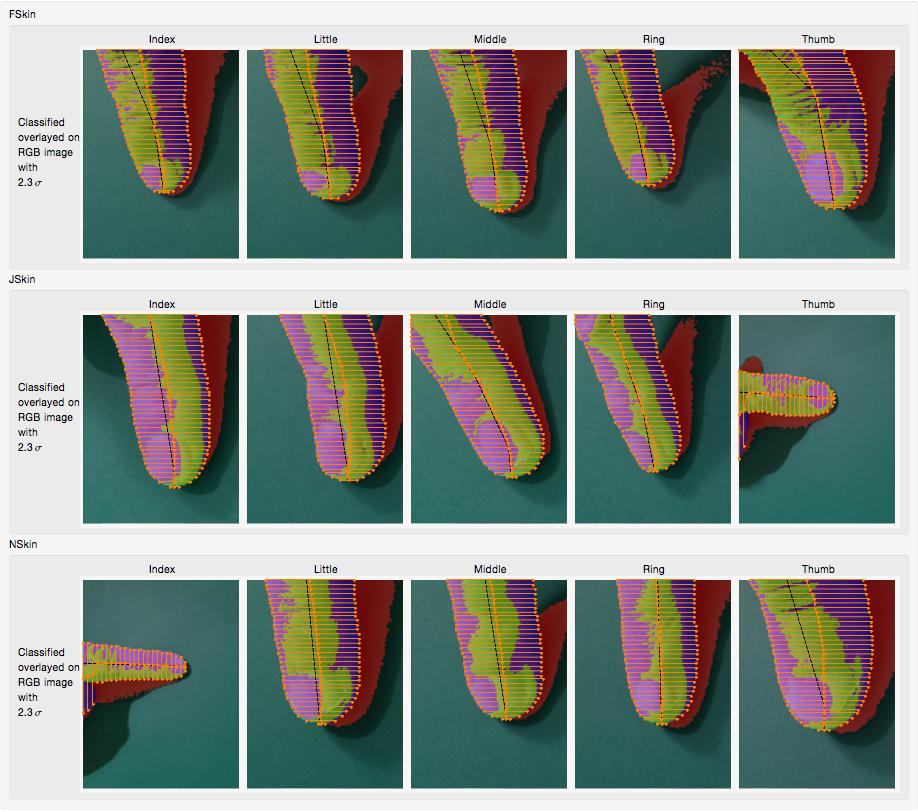
\includegraphics[width=0.95\textwidth]{Chapter4/Figs/FillamentFill.jpg}
    \caption{The 'Filament Fill' Method.}\label{fig:FillamentFill}
\end{figure}

The Filament Fill method takes a path --- given as a sequence of points --- within an object and finds the edges of the object using the Hurdle method running away from the path within the object. Assuming a horizontally-oriented object, the path's extent in the horizontal direction is divided equally into points, and these points are used to start the Hurdle method in the vertical directions, and vice versa for vertical-oriented objects.



For the purposes of the shape detection algorithms, there are metrics that are applied which suffer from noise and anomalies, where the noise is due to the natural variability of human digits from regular geometric forms, and the anomalies are due to misdetections of the edges of the digit. We assume that the anomalous results are extreme values, however we acknowledge that the most common (mode) or middle (median) values may not be representative of the best geometric approximation for the shape. The Mean-Median method --- similar to the "k-Nearest Neighbors" algorithm --- solves this problem by taking a confidence interval around the median and then taking the mean of the points within this interval. This method is a useful adaptation of methods like the k-Nearest Neighbors in that it solves the outlier problem for this particular application.

\subsection{The `Kink Fit' Method}\label{sec:KinkFitMethod}
The Kink Fit algorithm takes in a set of 2D points, where the first component is taken to be the independent variable and the second component is taken to be the dependent variable. This assumption excludes the possibility of truly vertical lines being presented to the algorithm. The Kink Fit algorithm fits a function which consists of two straight-line segments to a set of points. Unfortunately, currently the only piecewise linear fitting function is the proprietary MARS algorithm which, aside from being commercial, is overkill for this particular problem, which has a small number of points which are well-aligned. 

The Kink Fit algorithm relies on the fact that we know that the points are in order; it chooses a point and divides the set in two, and then performs a standard, least squares linear fit to the two sets. Both sets include the point at which the set is divided. 

The fit is also assumed to be continuous, except in the first derivative. The algorithm as described above may produce two lines which do not intersect between the second-to-last data point used for the first line and the second data point used for the second line. The algorithm needs to ensure that this is the case. This is achieved by shifting the second half of the data set by the end point of the linear fit to the first half of the data set. The point at which the two linear fits intersect is found, and if that point is between the second-to-last point in the first set, and a second point in the second set (i.e. the points on either side of the point of division), then the fit is considered to be acceptable. If the fit is not acceptable, it indicates that there's a discontinuity in position rather than simply being a discontinuity in the first derivative. This is handled by choosing the point on the fit to the first set closest to the intersection within the bounds of the points on either side of the point of division. The linear fit is then performed with only the gradient as the free parameter, guaranteeing that the line will have passed through this limiting point.

The algorithm then finds the residuals, and then finds the average of the square of the residuals. This is considered the score for dividing the set of points at that position. The algorithm finds the point which minimizes the score using a bisecting algorithm; if a linear fit to the data has a low score, then the Kink Fit algorithm is considered unnecessary and the digit is assumed to be in a relaxed, straight, neutral pose. The algorithm specifies a minimum number of points to be included in a set, as this avoids the problem of dividing into sets which contain only one point.

\subsection{The `Elliptical Fit' Method}\label{sec:EllipticalFitMethod}
Fitting an ellipse to a set of points is surprisingly difficult. The reason for this is outlined below.

To follow the standard linear algebra approach to least squares fitting, we need to decide upon a functional form for the fit, and thereby a basis set. For an ellipse, this basis set is $\chi= \left(x^2, x y, y^2, x, y, 1\right)$, which is a set of six free coefficients $ A^T=\left\{A_{\text{xx}},A_{\text{xy}},A_{\text{yy}},A_x,A_y,A_0\right\}$. However, to specify an ellipse, all that is needed is five numbers; the major and minor axes lengths $(a,b)$, the position $(x_0,y_0)$, and the orientation $\theta$. This is because the basis set includes lines, quadratics, parabolic and hyperbolic functions as well as elliptical functions as possible fits. An additional difficulty arises when we try to construct a cost function for an ellipse. Ideally, we wish to minimize the perpendicular distances of the points from the ellipse, but the calculation of the distance of a point from an ellipse is not straightforward, requiring the roots of a fourth degree polynomial to be found. Due to these complexities, several different methods have been proposed by different authors, but we will be focusing on two methods: The Approximate Mean Square (AMS)  proposed by (\cite{Taubin1991}), and the Direct least square (Direct) method by (\cite{Fitzgibbon1999}).


For the fingertip problem, there is also the added difficulty that the points are confined to one side of the ellipse so we have chosen methods which cope well with partially occluded ellipses. Both methods begin by forming the design matrix and then applying an additional constraint which restricts the fit to a family of curves. Both methods are formulated as generalized eigenvalue problems, avoiding the need for iterative methods.

The AMS method restricts the fit to parabolic, hyperbolic and elliptical curves by imposing the condition that $ A^T ( D_x^T D_x  +   D_y^T D_y) A = 1$ where the matrices $Dx$ and $Dy$ are the partial derivatives of the design matrix $D$ with respect to x and y. The matrices are formed row by row applying the following to each of the points in the set:
\begin{align*}
D(i,:)&=\left\{x_i^2, x_i y_i, y_i^2, x_i, y_i, 1\right\} &
D_x(i,:)&=\left\{2 x_i,y_i,0,1,0,0\right\} &
D_y(i,:)&=\left\{0,x_i,2 y_i,0,1,0\right\}
\end{align*}
The AMS method minimizes the cost function
\begin{equation*}
\epsilon ^2=\frac{ A^T D^T D A }{ A^T (D_x^T D_x +  D_y^T D_y) A^T }
\end{equation*}

The minimum cost is found by solving the generalized eigenvalue problem.

\begin{equation*}
 D^T D A = \lambda  \left( D_x^T D_x +  D_y^T D_y\right) A 
\end{equation*}

The Direct method confines the fit to ellipses by ensuring that $4 A_{xx} A_{yy}- A_{xy}^2 > 0$. The condition imposed is that $4 A_{xx} A_{yy}- A_{xy}^2=1$ which satisfies the inequality and as the coefficients can be arbitrarily scaled is not overly restrictive.

\begin{equation*}
\epsilon ^2= A^T D^T D A \quad \text{with} \quad A^T C A =1 \quad \text{and} \quad C=\left(\begin{matrix}
 0 & 0  & 2  & 0  & 0  &  0  \\ 
 0 & -1  & 0  & 0  & 0  &  0 \\ 
 2 & 0  & 0  & 0  & 0  &  0 \\ 
 0 & 0  & 0  & 0  & 0  &  0 \\ 
 0 & 0  & 0  & 0  & 0  &  0 \\ 
 0 & 0  & 0  & 0  & 0  &  0 
\end{matrix} \right)
\end{equation*}

The minimum cost is found by solving the generalized eigenvalue problem.

\begin{equation*}
 D^T D A = \lambda  \left( C\right) A 
\end{equation*}

The system produces only one positive eigenvalue $ \lambda$ which is chosen as the solution with its eigenvector $\mathbf{u}$. These are used to find the coefficients

\begin{figure}[p]
\centering
\subfloat[Comparison of the AMS and Direct ellipse fit methods for a complete ellipse][AMS and Direct methods both perform well with a set of points evenly distributed arround the ellipse. ]{
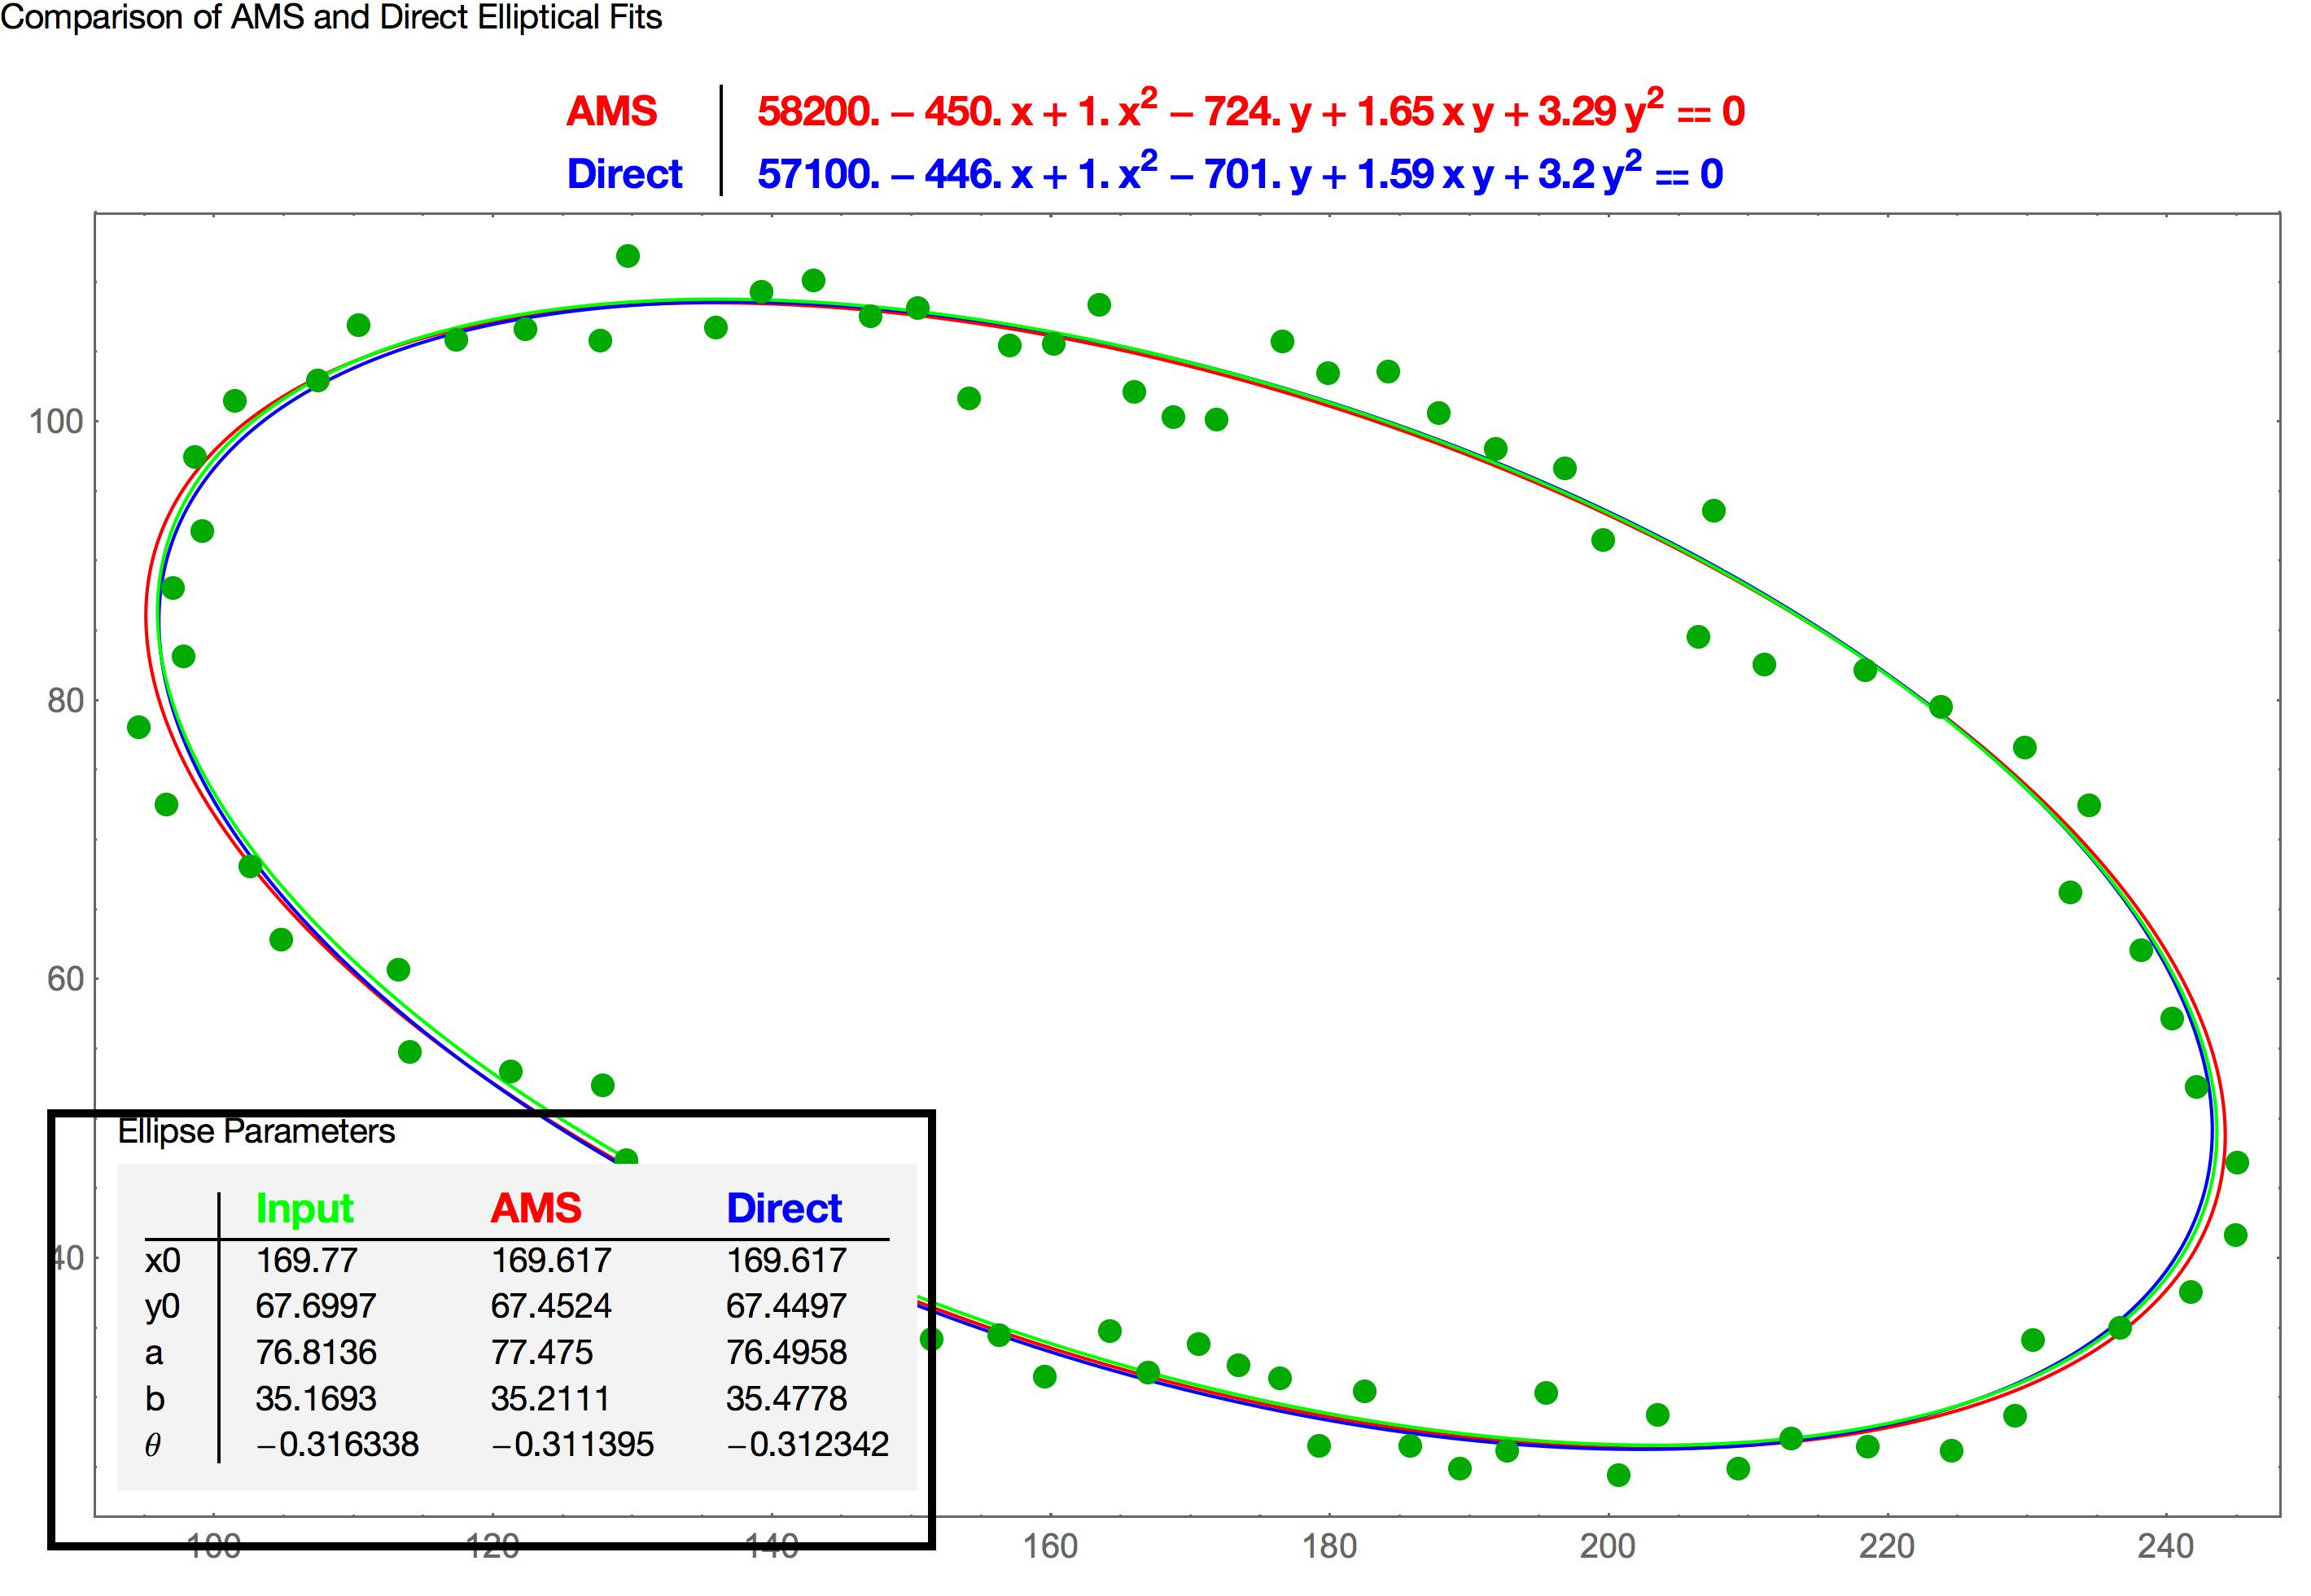
\includegraphics[width=0.98\textwidth]{Chapter4/Figs/EllipticalFitTestFull.jpg}
\label{fig:EllipseFitTestFull}}
\qquad
\subfloat[The AMS method sometimes produces a hyperbolic fit.][The AMS method sometimes produces a hyperbolic fit whilst the direct method always produces an ellipse]{
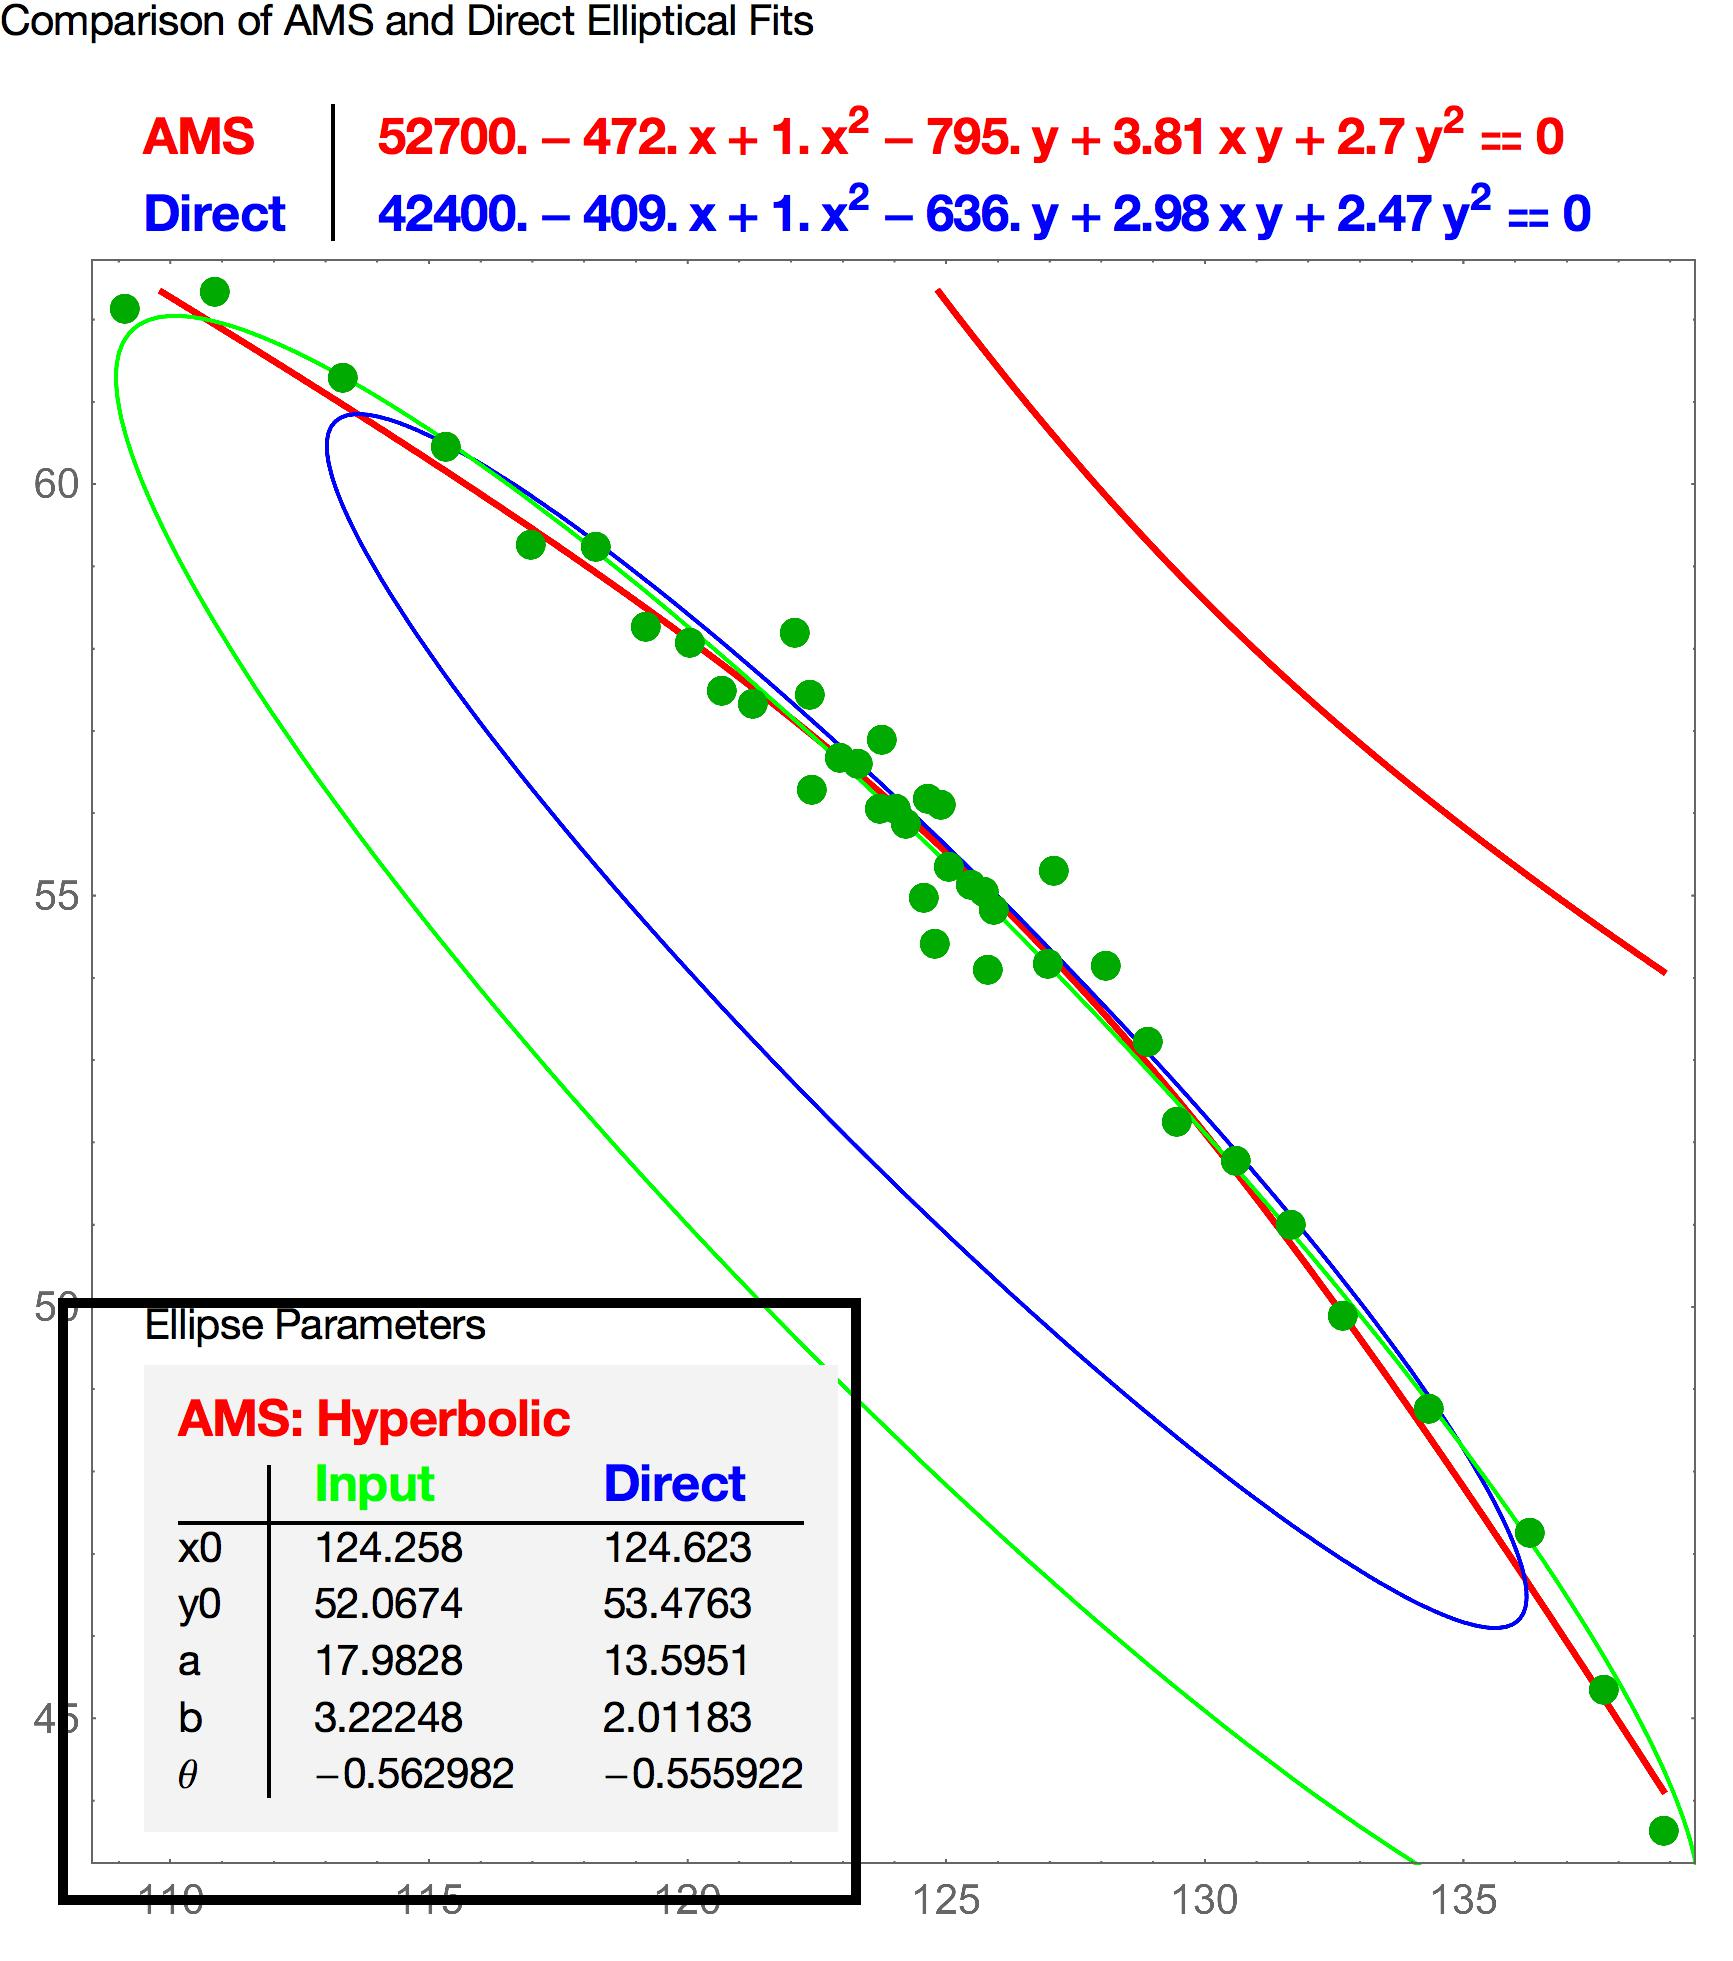
\includegraphics[width=0.47\textwidth]{Chapter4/Figs/EllipticalFitTest_Hyperbolic.jpg}
\label{fig:EllipseFitTestHalfHyperbolic}}
\quad
\subfloat[Comparison of the AMS and Direct ellipse fit methods for a half ellipse.][The AMS method better fits the extreme edge points in the data set resulting in the AMS method producing larger ellipses than the Direct method. The true ellipse is most often between the  two.]{
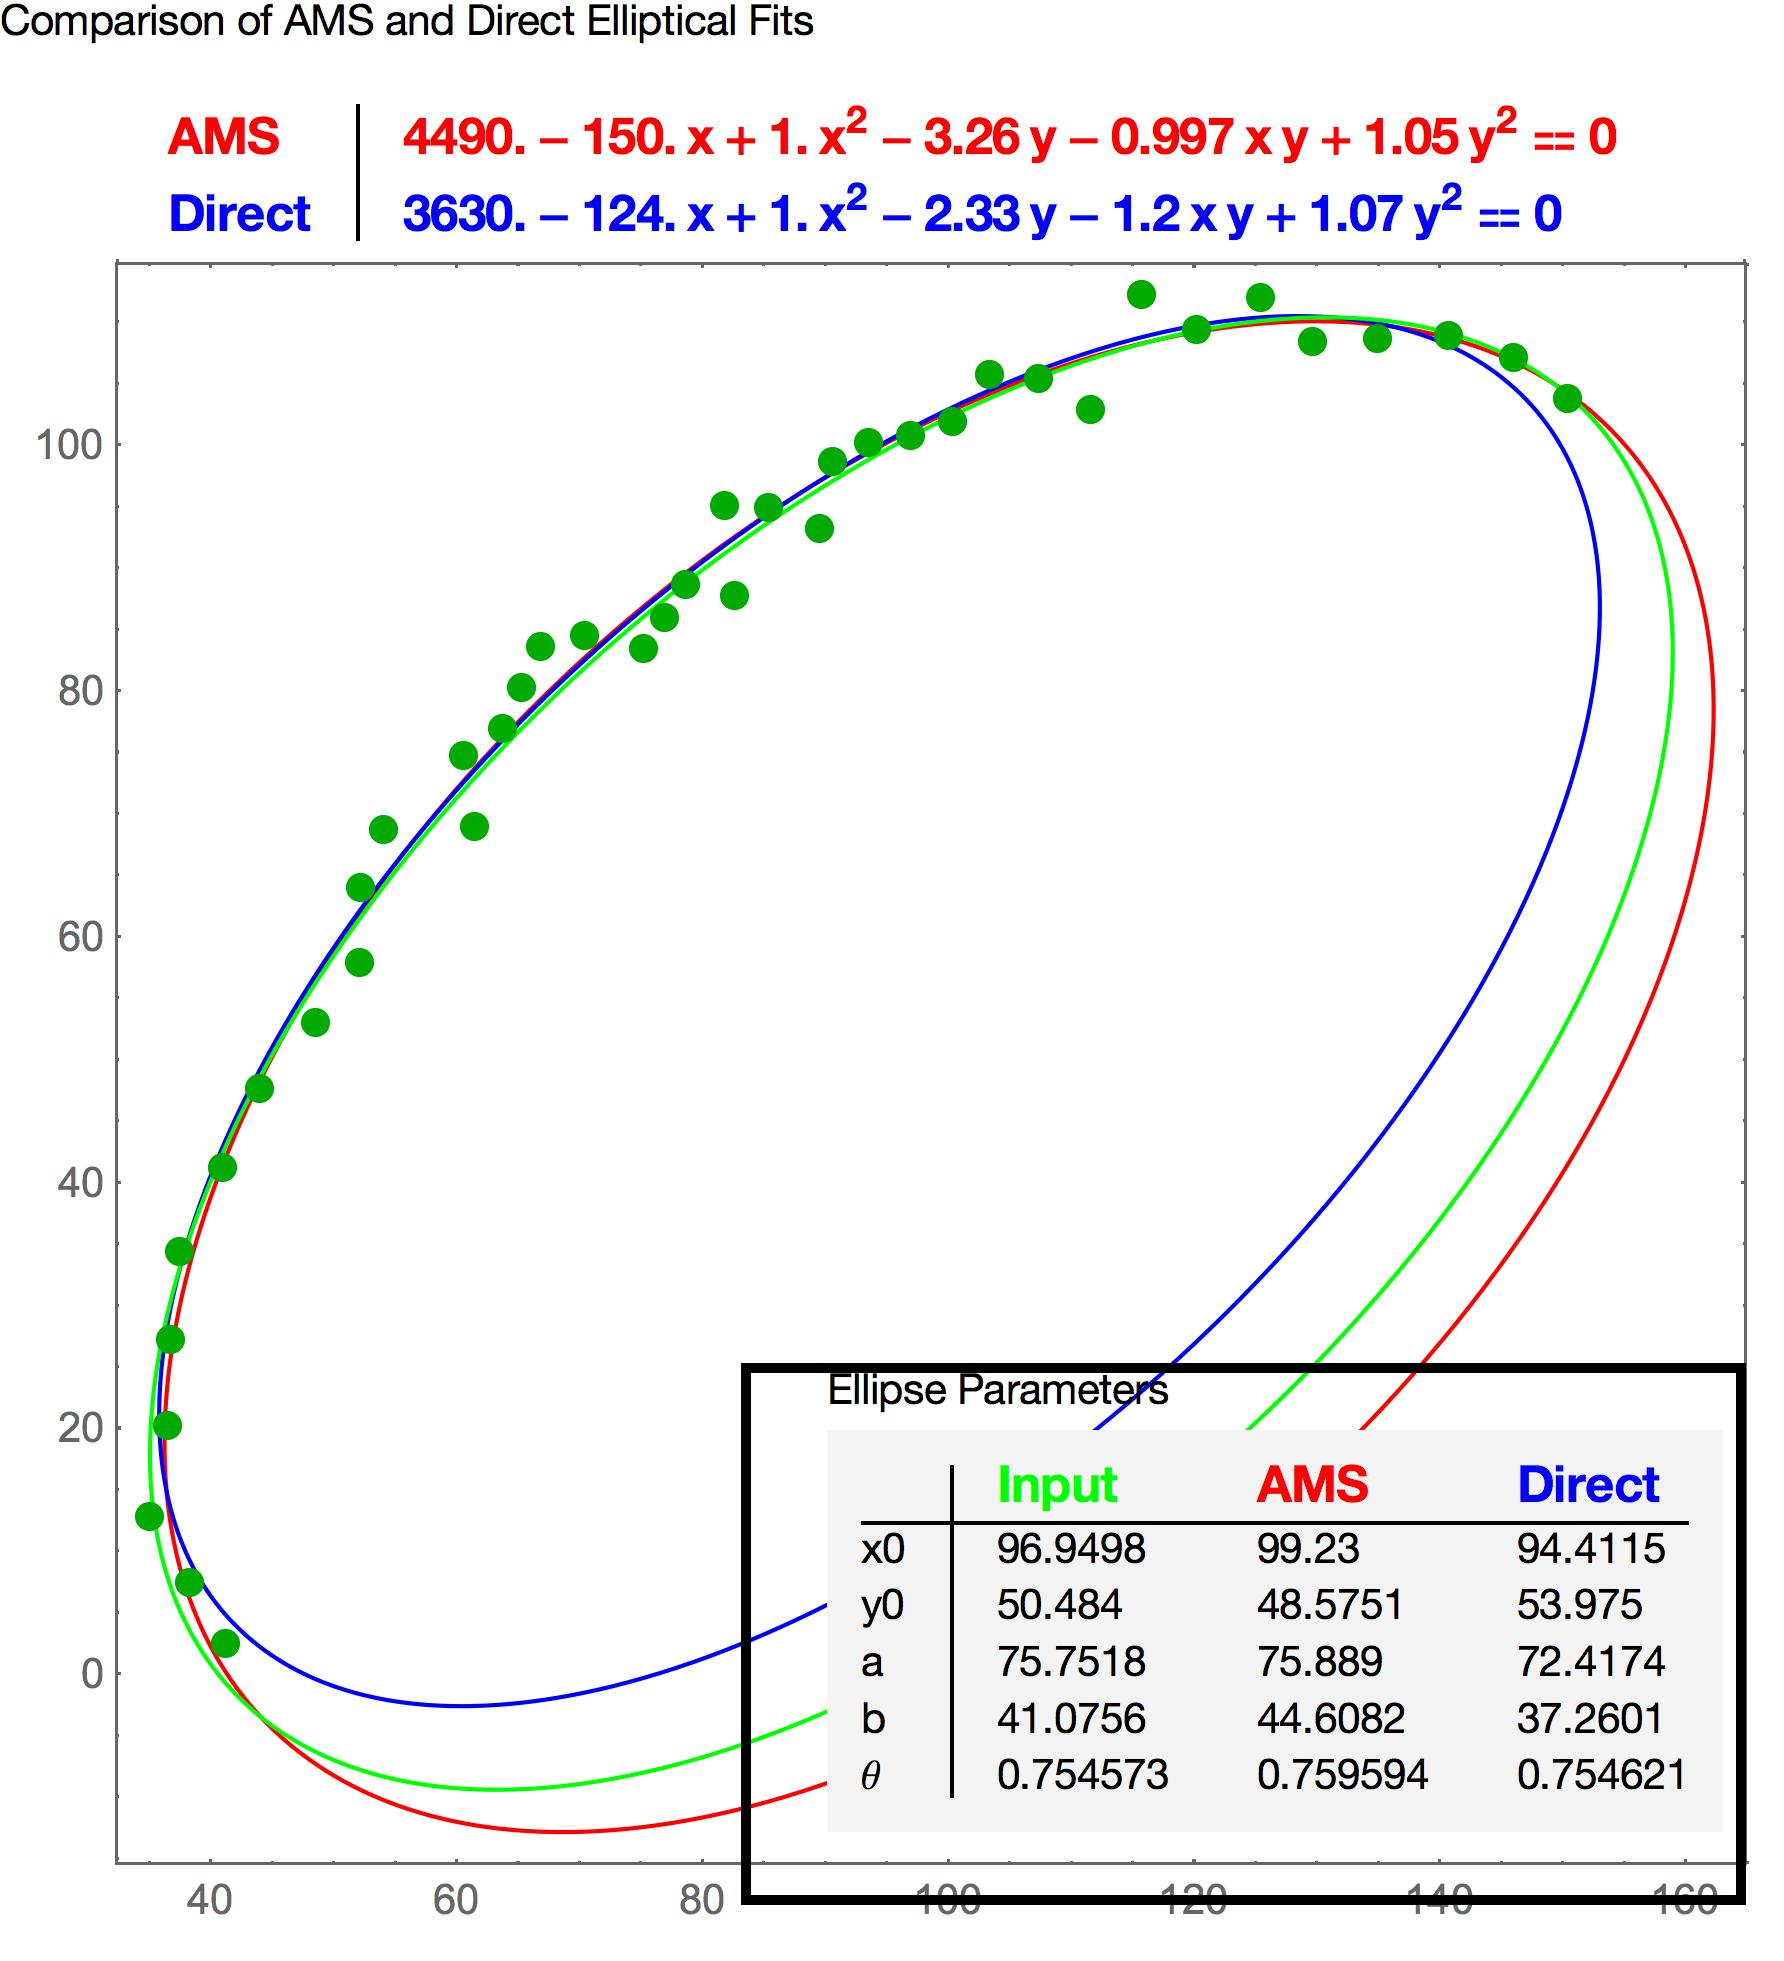
\includegraphics[width=0.47\textwidth]{Chapter4/Figs/EllipticalFitTest_DTA.jpg}
\label{fig:EllipseFitTestHalf}}
\caption{Comparison of the AMS and Direct ellipse fit methods.}
\label{fig:EllipseFitTest}
\end{figure}

\begin{equation*}
 A = \sqrt{\frac{1}{\mathbf{u}^T C \mathbf{u}}}  \mathbf{u}
\end{equation*}
The scaling factor guarantees that  $A^T C A =1$.

These methods were implemented in Mathematica for evaluation and in the OpenCV C++ code. Testing routines generated sample data with variable ellipse occlusion and noise around a randomly generated ellipse . The methods both produced good fits to complete ellipses Fig.\ref{fig:EllipseFitTestFull} and incomplete ellipses Fig.\ref{fig:EllipseFitTestHalf}. The AMS method was slightly better at fitting the extreme ends of the ellipse, generally producing a larger ellipse than the Direct method. Both methods accurately obtained the position and orientation. The AMS method occasionally produced a hyperbolic fit for very flat ellipses Fig \ref{fig:EllipseFitTestHalfHyperbolic}.


The largest computational effort in both methods is the determination of the $D^T D$ matrix. Once found, however, both methods can be used at relatively little extra computational cost. All Ellipses between the two can be considered as valid fits also. This suggests a method which allows for extra information to be used to refine the fit. In the case of the finger model this is the orientation, distal width and position from the parallel line fit. The ellipse between the two fits which most closely matches the extra information is chosen as the best fit.
\clearpage

\subsection{The `Isoscelian Trapezian' Fit}\label{sec:TrapezianFit}

Given three sets of points corresponding to the top, middle and bottom of an isosceles trapezium which is oriented so that the parallel sides are on the left and right, a fit can be found as follows:

\begin{enumerate}
\item A straight line fit to the midpoints is found giving start and end points along with an orientation.
\item The points are translated and rotated so that the first middle point is at the origin and the last middle point is on the x axis.
\item The bottom points are reflected about the x axis.
\item A single straight line is fitted to the top and reflected bottom points together.
\item Four points describing the trapezium are found and returned along with the orientation and position in the original coordinates.
\end{enumerate}

\subsection{The `Force Analogue Shape Detection' Method (FASDM)}\label{sec:ForceAnalogue}
\newcommand{\pos}{\mathbf{P}}
\newcommand{\F}{\mathbf{F}_i}
\newcommand{\Ft}{\mathbf{F}^\tau_i}
\newcommand{\dm}{\mathbf{d}^{m{\scriptscriptstyle dl} }_i}
\newcommand{\di}{\mathbf{d}^{i{\scriptscriptstyle mg} }_i}
\newcommand{\Mt}{\mathbf{\tau}_i}
The FASDM is one of the most straightforward --- if not the most straightforward --- shape alignment algorithms. Given a set of points, if we know a corresponding set of points on the the target shape model, we can find translation vectors between the points on the model $\dm$ and the points  on the image $\di$; the FASDM makes the analogue between these vectors and a force acting on that point on the model $\F=\di-\dm$. The position and orientation of the shape is then found by translating and rotating the model such that the 'force' acting upon it sums to zero. To facilitate the calculation the model is expressed in coordinates where the origin corresponds to the center of mass for the model.

It should be noted that other transformations can easily be included, however for the current purposes, rotation and translation are all that is required.
The translation vector $\F$ is found by taking the average of the force acting on the center of mass $\pos= \frac{1} {n} \sum_{i=1}^n \F$. 
Translating the model to this position allows the residual turning forces to be found $\Ft = \F - \pos$. 
The moment about the center of mass $\Mt$ is found simply by finding the magnitude of the outer product of the residual turning force $\Ft$ with the the point on the model $\dm$ thus $\Mt = \lVert \Ft \wedge \dm \rVert$. 
The rotation which would reduce the moment to zero is found by taking the angle between $\dm$ and $\dm+\Ft$.
The moment weighted average of these is the angle $\theta$ which will most reduce the total rotational moment $\mathbf{\tau} $. 

\begin{align*}
\theta &= \frac{1} {\mathbf{\tau}} \sum_{i=1}^{n} \Mt \theta_i &
\theta_i &=  \arccos \left(\frac{\dm \cdot (\dm+\Ft)}{\lVert \dm \rVert \lVert \dm+\Ft \rVert}\right)  &
\mathbf{\tau} &= \sum_{i=1}^{n} \Mt \\
\pos &= \frac{1} {n} \sum_{i=1}^n \F &
  &=  \arccos \left(\frac{\dm \cdot (\di - \pos)}{\lVert \dm \rVert \lVert \di - \pos \rVert}\right)  &
\Mt &= \lVert (\di - \pos) \wedge \dm \rVert
\end{align*}

\begin{figure}[h!]
  \centering
    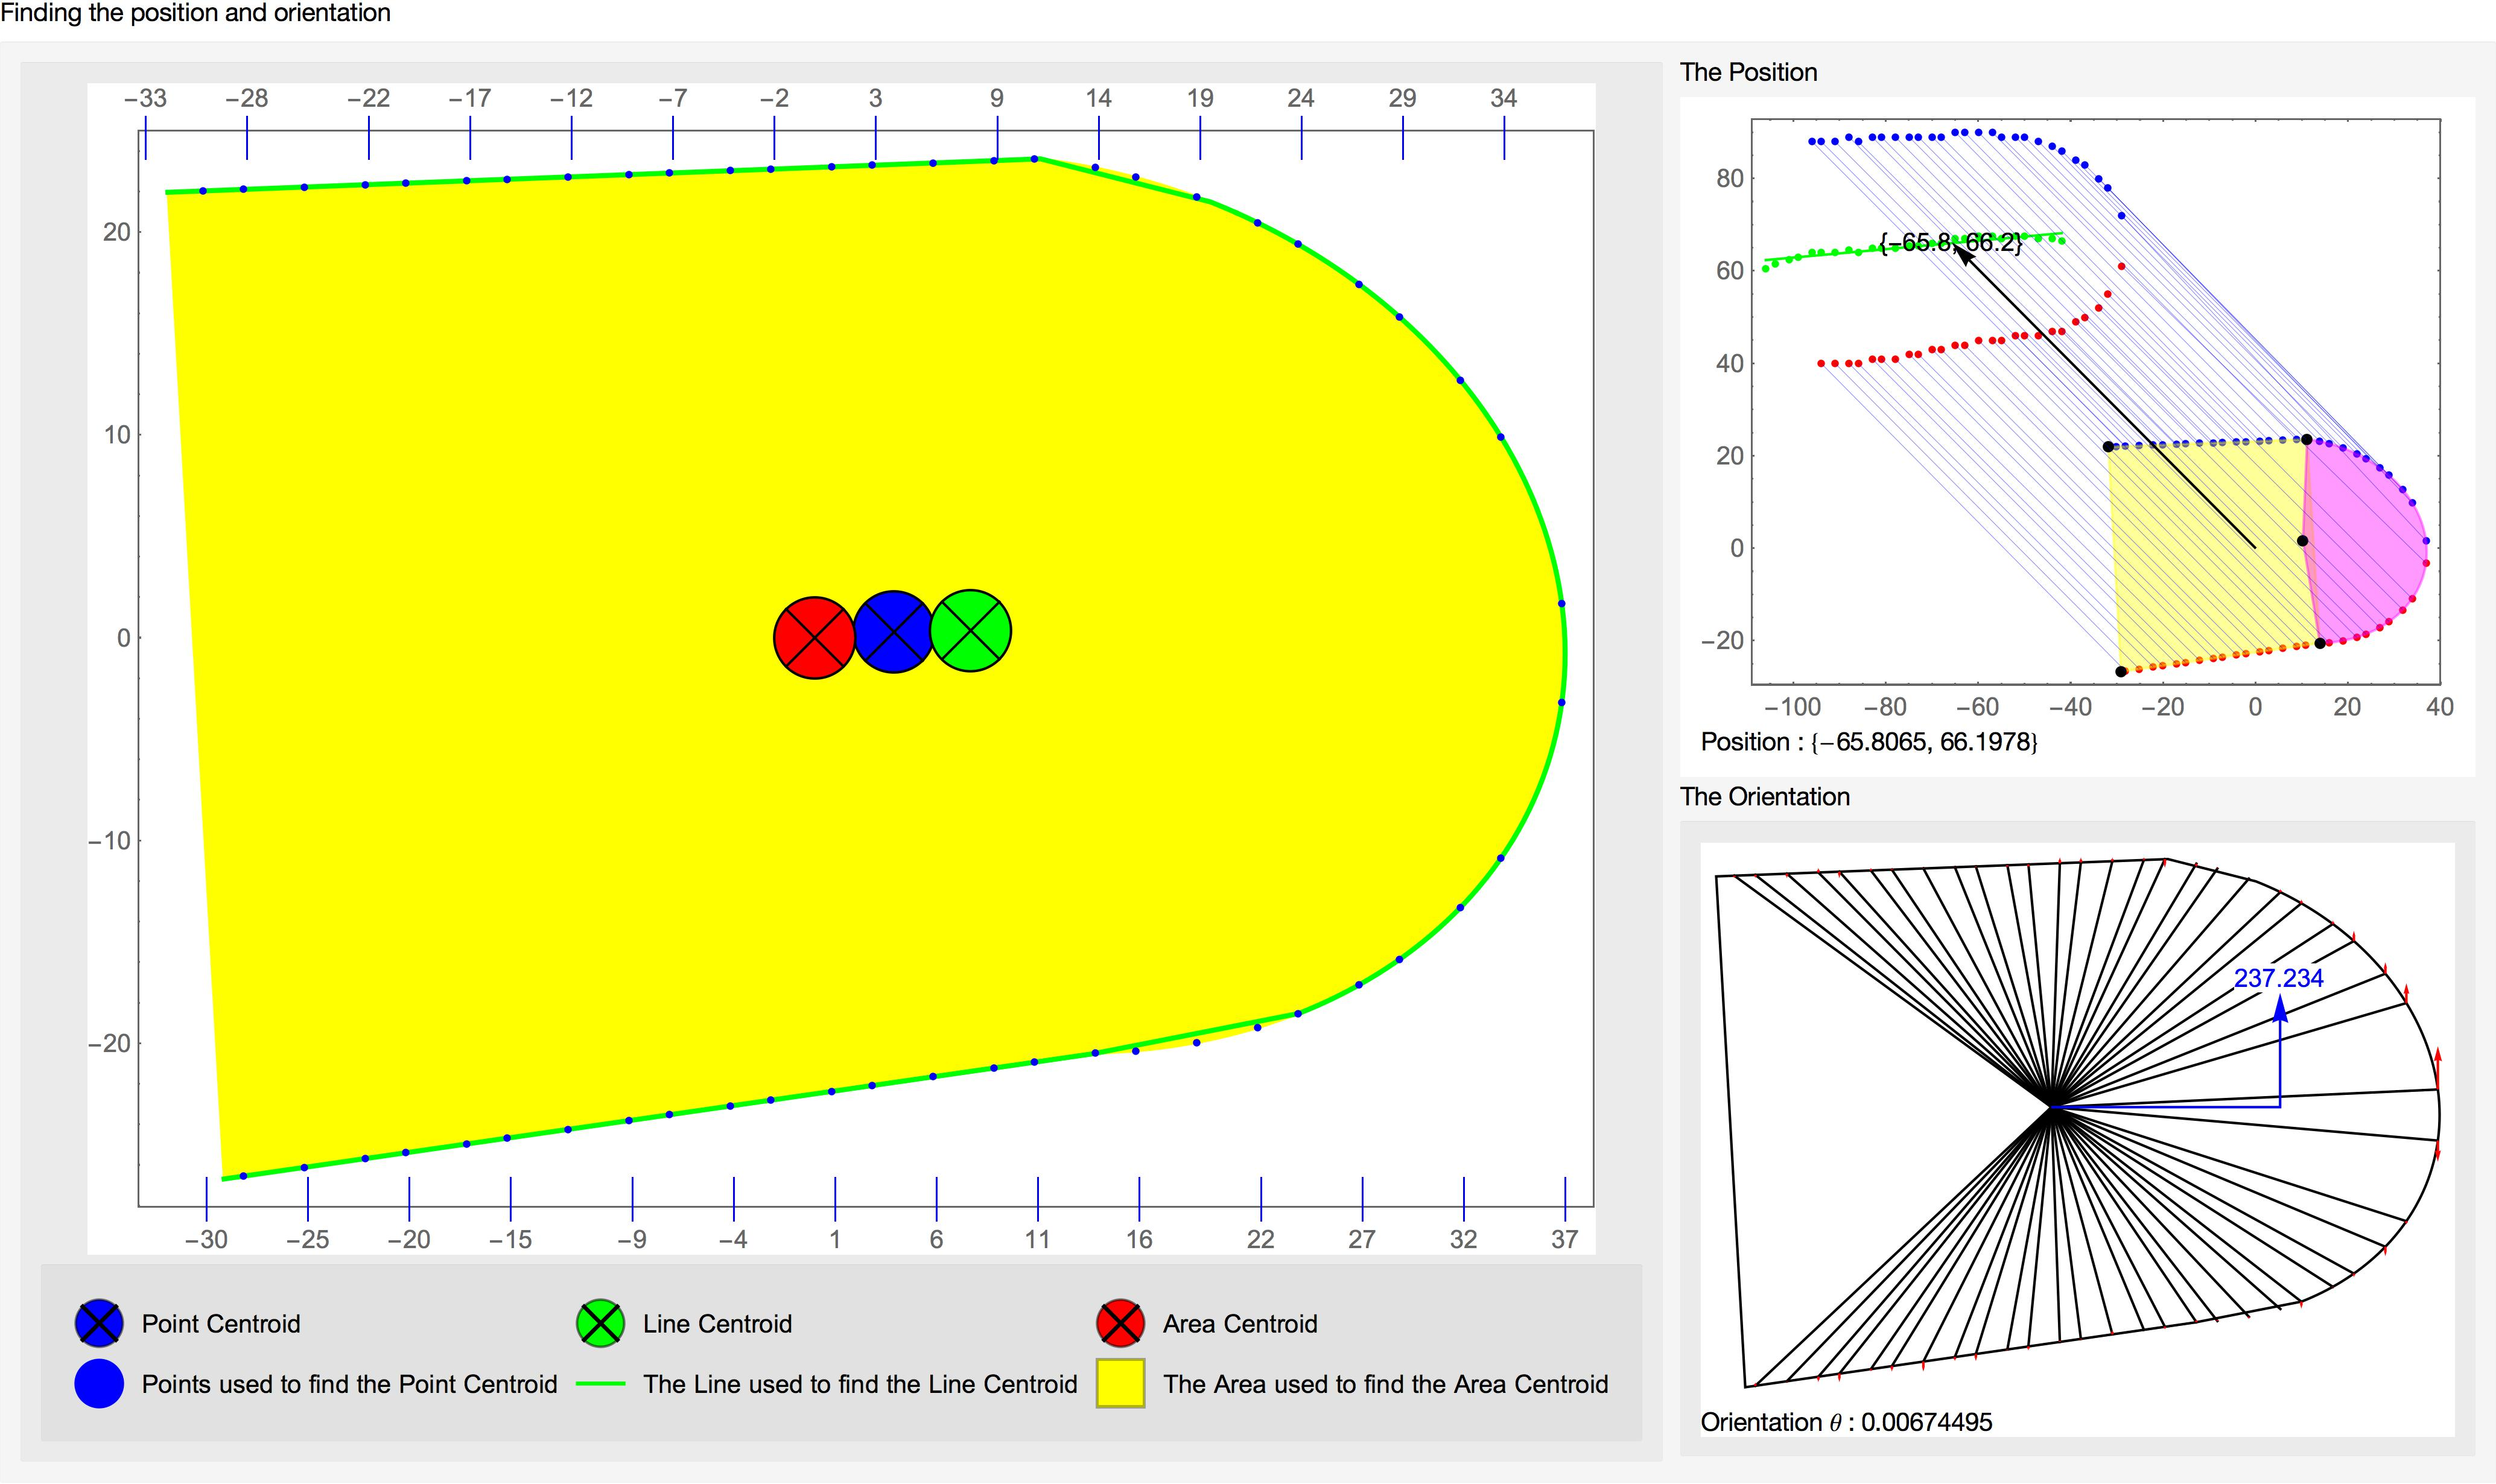
\includegraphics[width=0.95\textwidth]{Chapter4/Figs/Model_Centroids.jpg}
    \caption{Model Centroids.}\label{fig:ModelCentroids}
\end{figure}

\begin{figure}[h!]
  \centering
    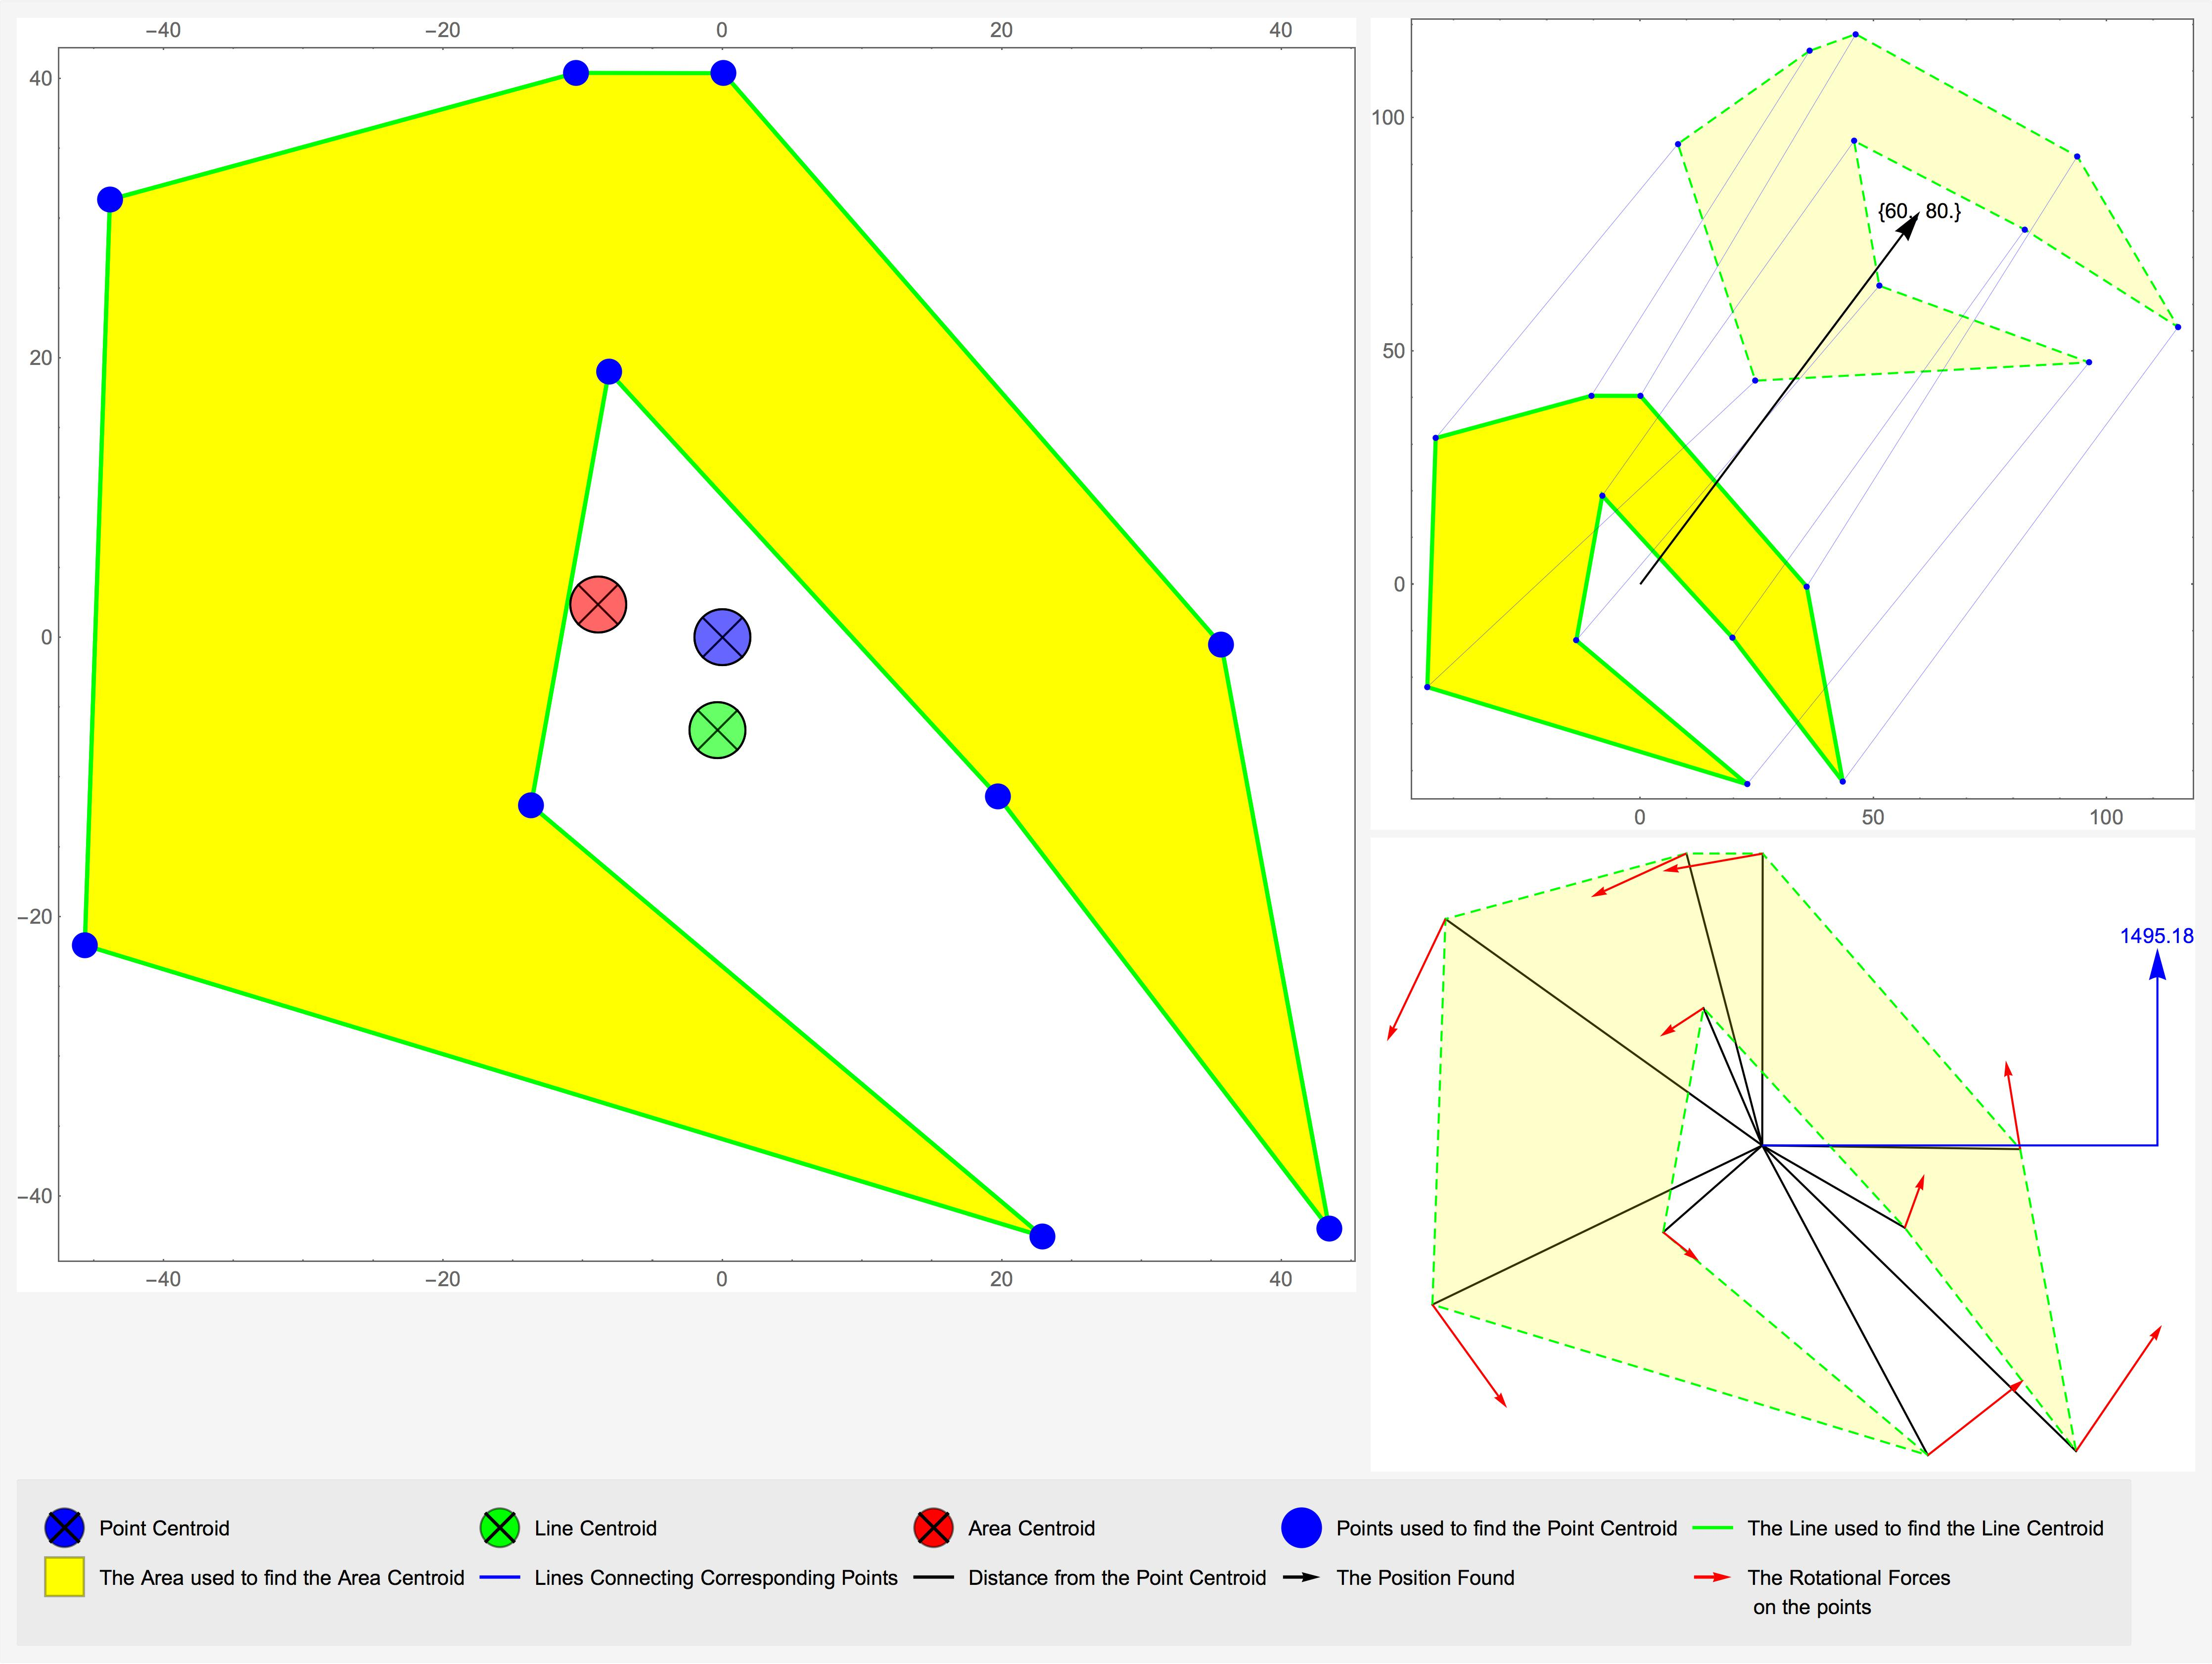
\includegraphics[width=0.95\textwidth]{Chapter4/Figs/Random_Polygon_Centroids.jpg}
    \caption{Random Polygon Centroids.}\label{fig:RandomPolygonCentroids}
\end{figure}

\begin{figure}[h!]
  \centering
    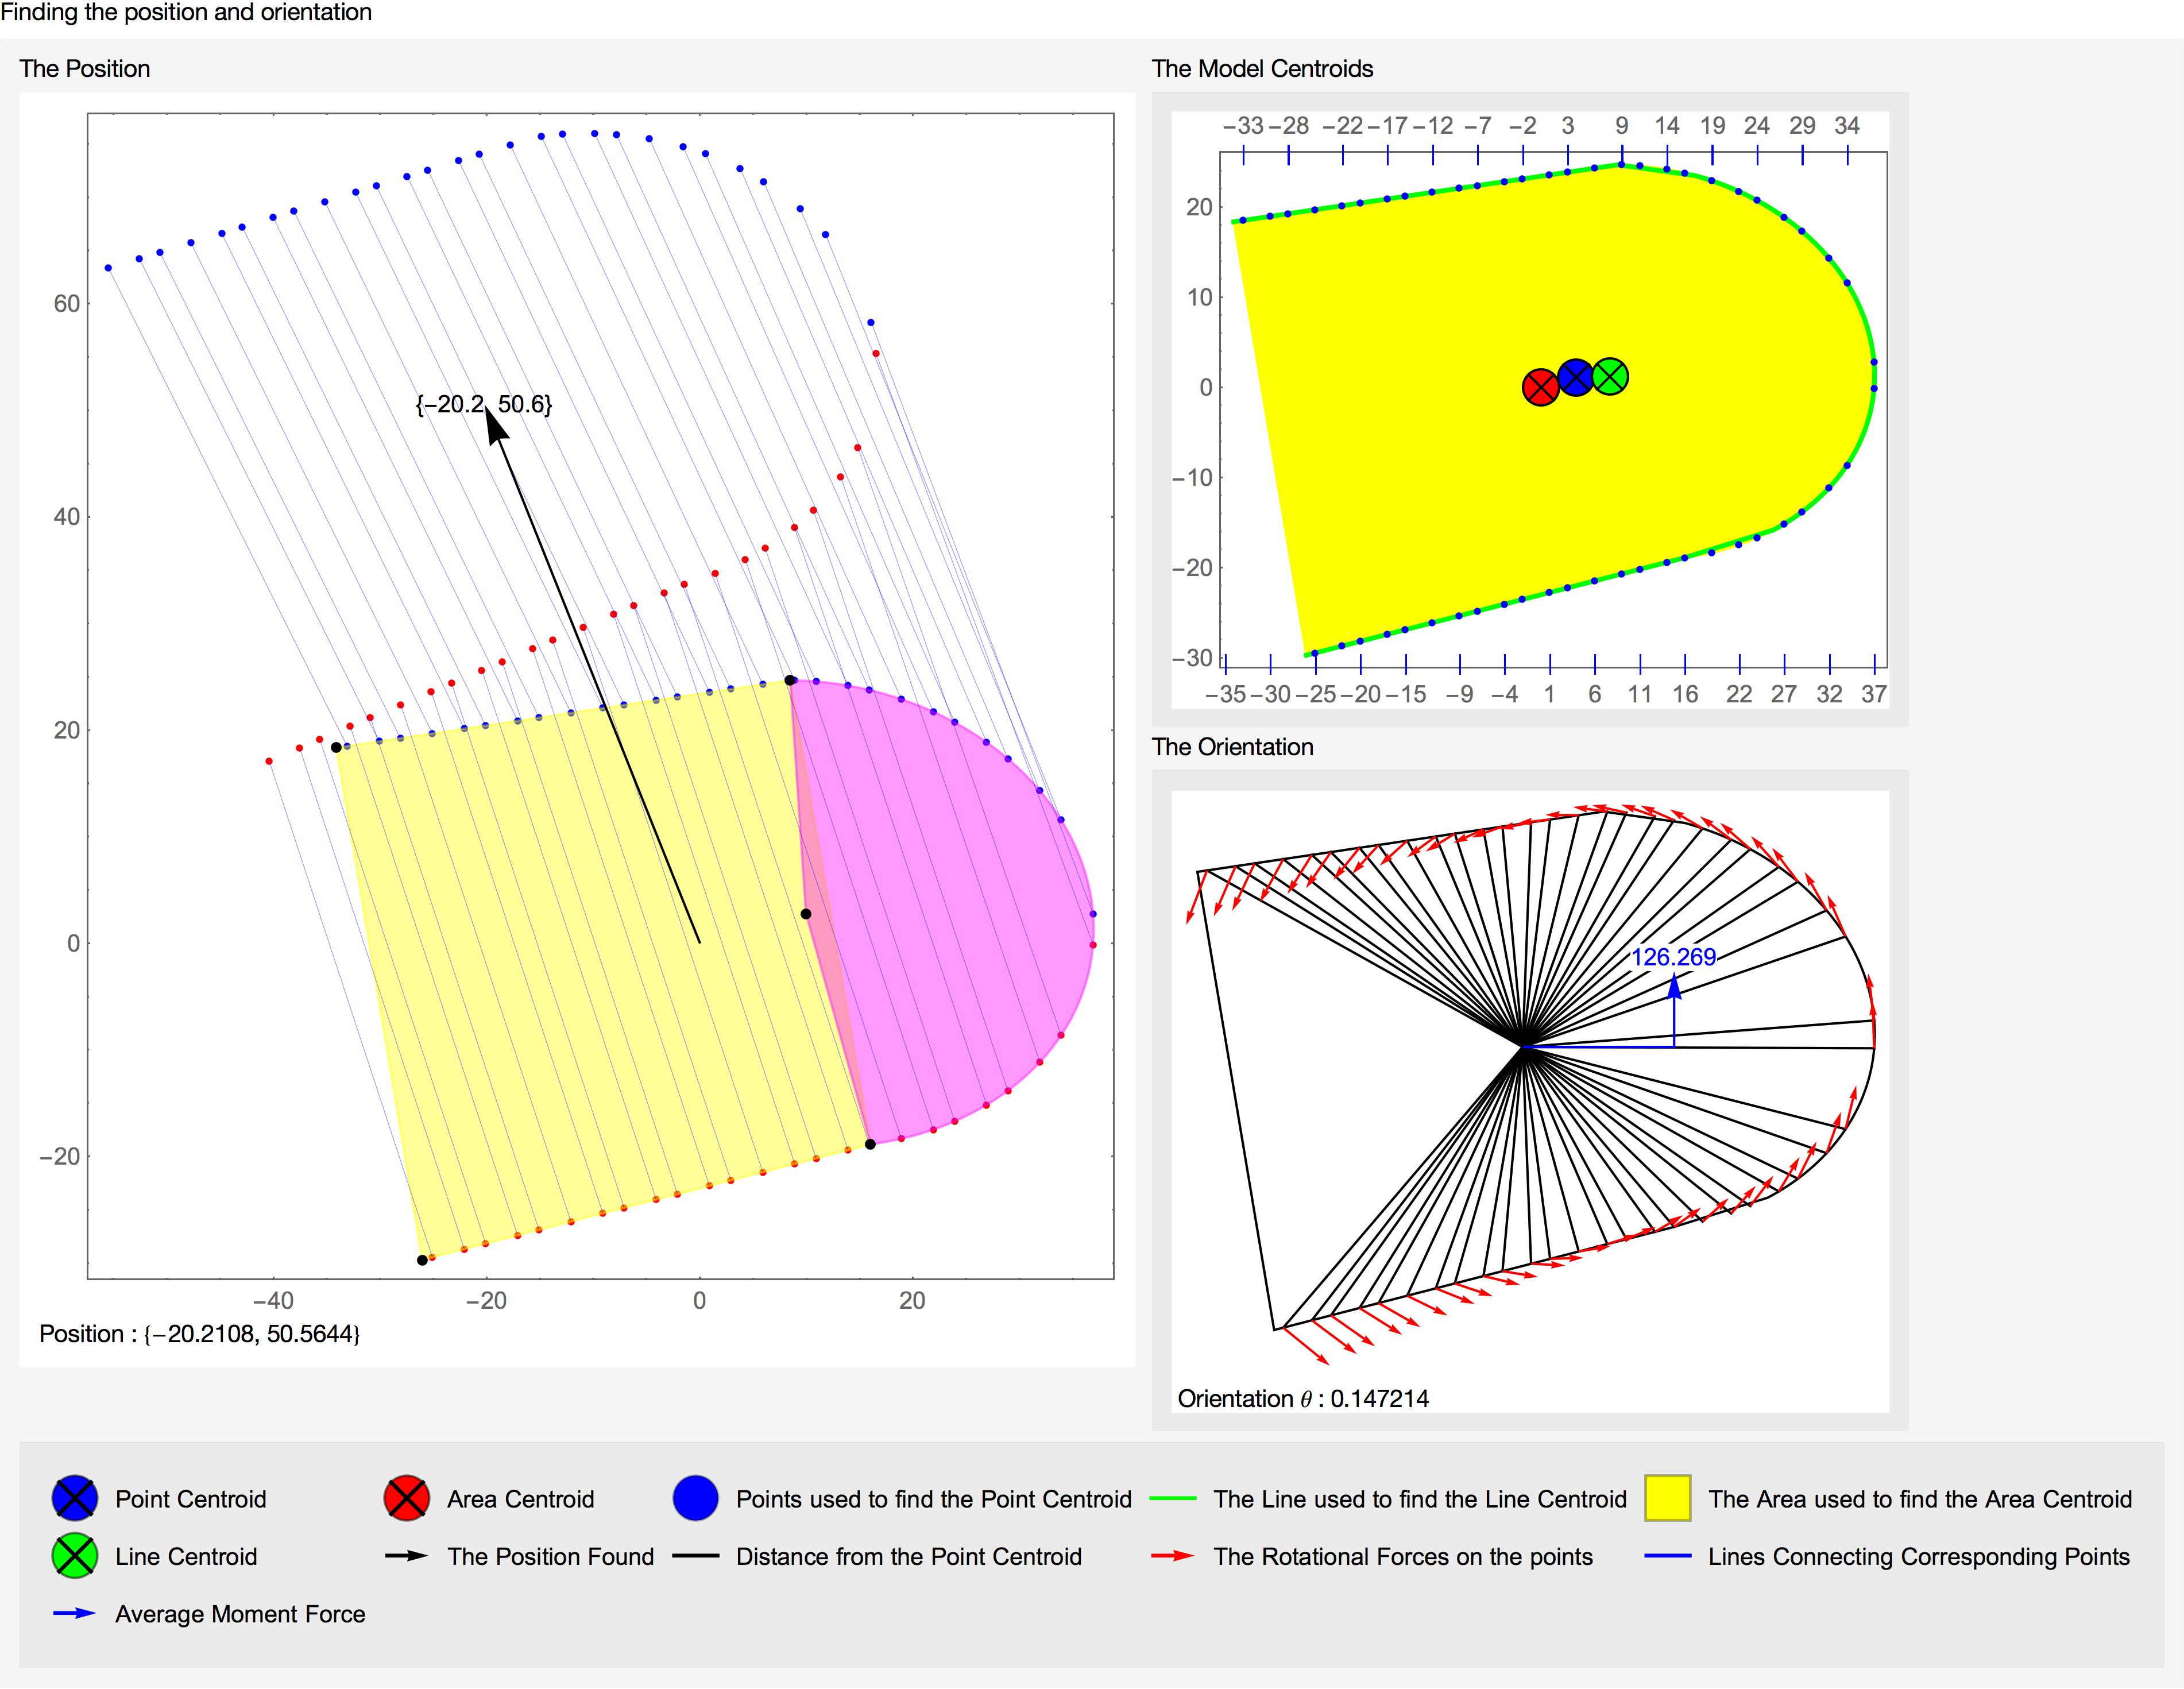
\includegraphics[width=0.95\textwidth]{Chapter4/Figs/Exagerated_Model_Centroids_With_Pos_Orientation.jpg}
    \caption{Position and Orientation.}\label{fig:ExaggeratedPositionAndOrientation}
\end{figure}

 Mathematically and algorithmically, there are three points which may be considered the center of mass: the centroid of the area of the model, which is where the center of mass would be if the model were a a flat, uniform sheet; the centroid of the perimeter of the model, which is the center of mass would be if the model were constructed using wire along the perimeter; and the arithmetic average of the points of interest defined on the perimeter of the model. The choice for the analogue of the center of mass depends upon the algorithm used. For a method which returns points radially distributed about a point in the model would favor the area centroid; a method which returned points relatively evenly distributed along the perimeter would naturally favor the perimeter centroid method; and a method which returned points of interest would favor the point centroid method. (There's no guarantee the points of interest would be distributed in any relation to the shape-based centroids.)


\section{Fingertip Model}\label{sec:FingertipModel}

We need an appropriate finger model so we can accurately align points on the fingertip between successive images in the video stream. We need to do this because otherwise, any difference between the frames will be overwhelmed by physical movement of the digit rather than movement of the blood inside the digit. For this reason, we target the most stable portion of the finger: the nail.

A digit has two joints and three segments: the distal, the middle, and the proximal. Each segment is roughly approximated by a rectangle, and the length of each section approximately following a 2-3-5 ratio, with lengths counting from distal to proximal, and where 1 is the $\frac{3}{4}$ width of the middle segment. Our finger model then comprises of the lengths and widths of each segment, the positions of the joints (i.e. {\tiny {\tiny }}the knuckles) between each segment, the position of the tip, and a position in the model marking the point at which the digit goes out of frame.

Given the width of the middle segment, we can then have an initial guess that the length of the distal segment is 1.5 times the initial width, the middle is 2.25 times that, and the proximal is 3.75 times that. Additionally, the center of the nail feature is not in the center of the distal segment, but a half unit (in our model units) away from the tip. The model can be laid out in units relative to the width of the digit.
\subsection{The Finger Shape Detection Algorithm}\label{sec:FingerShapeDetectionAlgorithm}

\subsubsection{Scale Space}\label{sec:ScaleSpace}
The images captured with the iPhone camera are extremely large, and so for the development of the algorithm, we define three scale spaces: one is the original image; two is an image size which represents the tip of the finger regardless of the distance of the camera from the finger, i.e. a scale relative to the width of the finger in the frame of the camera; three is a small image size for tracking the finger where it's freely roaming in the camera's view. We want these images to be formed without the need for resampling. For that reason, we restrict the choice of image sizes to those which are integer factors of the image dimensions. This is done by finding the integer factors of the original image dimensions and then selecting from those factors to scale the image. It should be noted that, to simplify point correspondences, the integer scaling from the small to medium scales is also kept.

\subsubsection{Finding the Frame Orientation}\label{sec:FindingTheFrameOrientation}
It is assumed we will not be using severed fingers, and so we know that the finger must exit the camera frame; the first step of the algorithm is then to detect which of the four edges the finger is entering from. This is done simply by finding the longest on-object path running along the frame sides. So, the algorithm starts by looking down the pixels on a frame side; when it locates a high-quaternary value, it uses the Hurdle method to find the longest path in that direction starting from that point. It continues around all four sides; the longest path found by the Hurdle algorithm is assumed to correspond to the finger entering the frame. From this, we set a frame orientation, which is the angle necessary to rotate the image such that the finger will be entering the frame from the left, and we set a direction vector pointing inwards from the frame edge found.

\subsubsection{Finding the End of the Finger Shape}\label{sec:FindingTheEndOfTheFingerShape}
Taking the longest Hurdle path on the frame edge found above, we take the middle point on that path and start a 'Run-Reach' algorithm in the direction found previously from that point. The Run-Reach algorithm proceeds as follows:

It finds a Hurdle path in the primary direction, i.e. perpendicularly away from the frame edge. At the end of the Hurdle path, it finds the Hurdle paths in the two perpendicular directions to its primary direction, i.e. parallel to the frame edge. It then finds the midpoint between the ends of the Hurdle path, and then uses that to start a new Hurdle path in its primary direction. The algorithm continues in this way until the end of the finger is found.

\begin{figure}[h!]
  \centering
    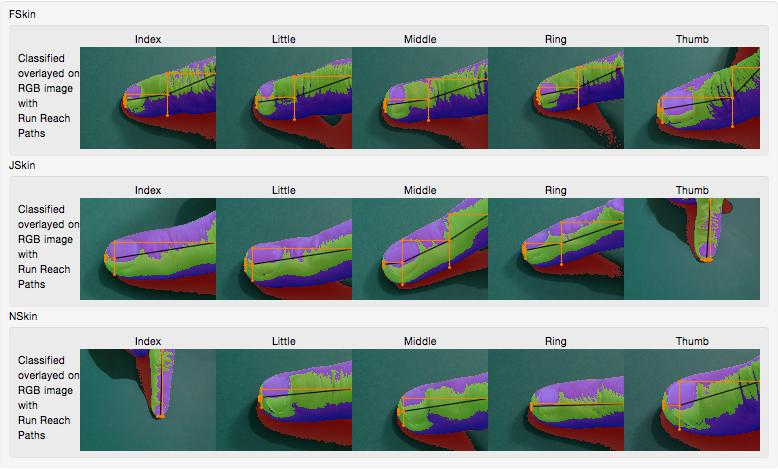
\includegraphics[width=0.95\textwidth]{Chapter4/Figs/FindingTheTip.jpg}
    \caption{Finding the End of the Finger Shape}\label{fig:FindingTheTip}
\end{figure}



\subsubsection{Filament Fill the Finger}\label{sec:FilamentFillTheFinger}
The center points found by the Run-Reach method above form a path on the finger. This is the path given to the Filament Fill method described previously. We now have a set of edge points on the digit. These edge points also have a top and bottom correspondence which, although they're not perpendicularly-opposite points on the finger, they do allow for a midpoint on the digit to be found. This can be seen in Figure~\ref{fig:FillamentFill}.

\subsubsection{Exclude Secondary Frame Edge Points and Fingertip Points }\label{sec:ExcludeSecondaryFrameEdgePointsAndFingertipPoints}
We need to exclude from the calculation of the midpoints on the digit values which are near the tip, and values which touch a second frame edge. This is because values toward the tip --- given that the finger is not necessarily perfectly horizontally-aligned --- give unreliable midpoint values because the Run-Reach path corresponds to shorter and shorter chords on a circle. Values which touch a second edge, more likely than not, do not correspond to the edge of the digit, but are simply where the digit exits the frame. (For example, JSkin Middle in Figure \ref{fig:ExcludedEdgePointsAndMidlineFit}.)

\begin{figure}[h!]
  \centering
    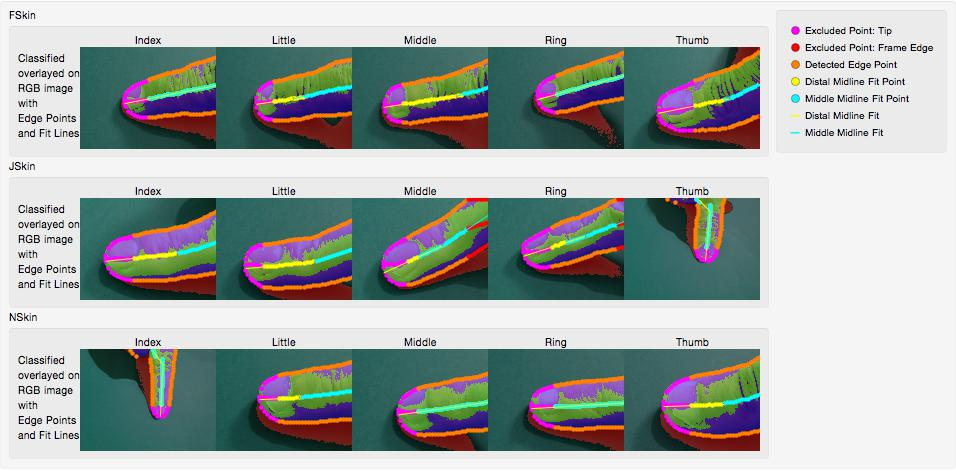
\includegraphics[width=0.95\textwidth]{Chapter4/Figs/ExcludedEdgePointsAndMidlineFit.jpg}
    \caption{Excluded Secondary Frame Edge Points and Fingertip Points, with the fit to the midline points returned by the Kink Fit algorithm.}\label{fig:ExcludedEdgePointsAndMidlineFit}
\end{figure}

To estimate which pairs of edge points correspond to points on the tip, the algorithm finds the length of the Hurdle path for all corresponding bottom-edge to top-edge points. These values are then sorted into ascending order, and then the 'Mean-Median' is taken, ensuring that the average is not affected by extreme values. The tolerance is determined by the algorithm by looking at the difference at the low and high ends of the $66\%$ range used by the Mean-Median.

\subsubsection{Kink Fit to the Finger}\label{sec:KinkFitToTheFinger}
We now have a set of reliable points at the midpoint of the finger. Because the finger is articulated, it is reasonable to assume that it may well be bent. We're interested in the action of the finger being pressed on a surface --- as a result, the finger is expected to be articulated at the distal-middle joint, but is otherwise straight. We wish to fit a function which consists of two straight-line segments to the set of reliable middle points. The fit was found using the 'Kink Fit' algorithm described in Section \ref{sec:KinkFitMethod}.

The Kink Fit algorithm as written takes a set of points where the first component is assumed to be the independent variable and the second component to be the dependent variable. However, because we haven't assumed that the finger comes into the frame from any particular direction, this can be problematic if, say, the finger comes through from the top or bottom of the frame, then the components would be in the wrong order for the Kink Fit algorithm to work. This is easily rectified by simply rotating the points into a standard orientation as if the finger is coming in from the left side of the frame. The computational effort in doing this is minimal because the number of points is small; we're not rotating the entire image, we're merely rotating a set of midline points, performing the Kink Fit algorithm, which returns a set of three points, which can then be rotated back to the original orientation.

In practice, however, the Kink Fit algorithm accepts the full set of midline points and a vector of pointers to the reliable values within that set. This allows the Kink Fit algorithm to extend out the end points of the line to the edges of the digit. Were this not the case, the end points returned would lie somewhere within the digit corresponding with the first and last reliable midline points. The result can be seen in Figure \ref{fig:ExcludedEdgePointsAndMidlineFit}.

\subsubsection{Parallel Lines Fit}\label{sec:ParallelLinesFit}
Our model of a finger assumes that the edges are parallel to each other. Since we have a line which runs through the center of the finger, we can now calculate the distance of the edge points to that line. These distances can be classified as good edge points if they're parallel to the central line. Whether they are parallel is determined by finding the Mean-Median distance from the central line to the edge points using a $50\%$ interval in the distal portion, because it is expected that up to half the points may be in the distal segment, maybe on the tip, and a $75\%$ confidence interval in the middle segment, because we expect fewer than $\frac{1}{4}$ of the edge points to be anomalies. The points are then classified as good if they are of Mean-Median distance from the central line. It should be noted that we consider both the top and bottom edges when calculating the Mean-Median distance. This technique successfully removes anomalies which are not parallel to the central line.

There is one final step: the points which are classified as good edge points are used to find a linear fit which is parallel to the central line. Finally, the width of the distal and the middle segments is calculated by finding the distance between these parallel lines. This can be seen in Figure \ref{fig:ParallelFit}.

\begin{figure}[h!]
  \centering
    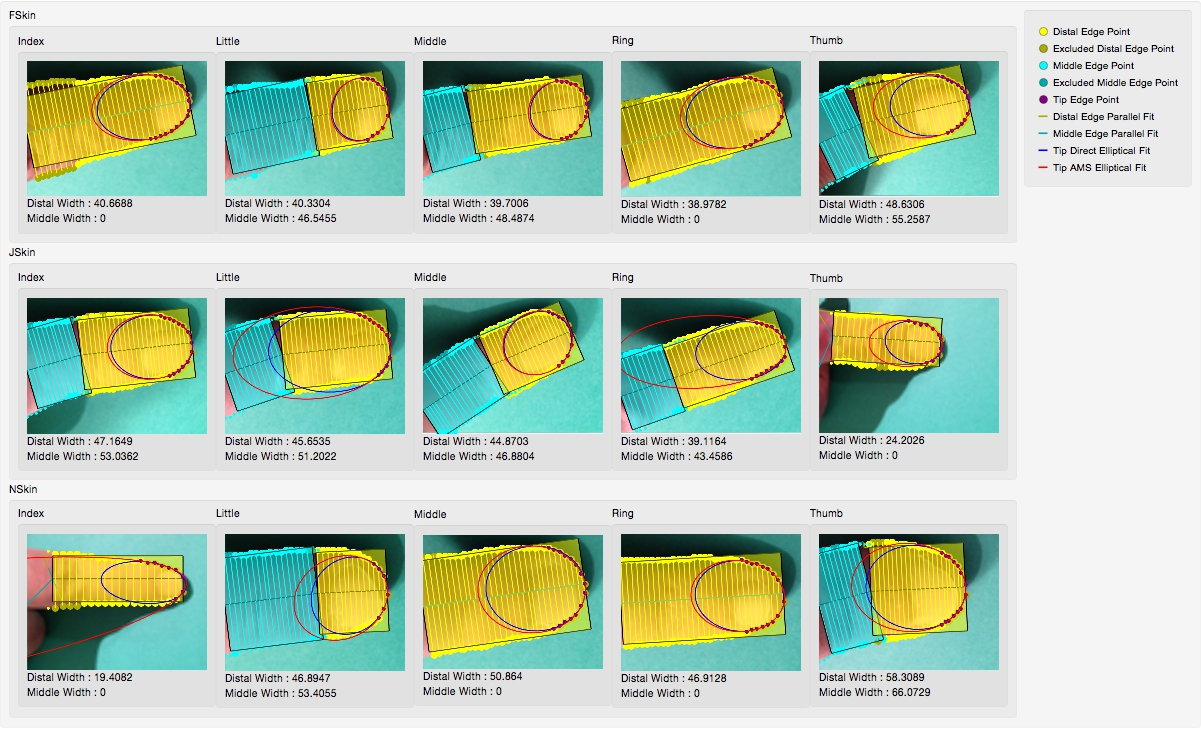
\includegraphics[width=0.95\textwidth]{Chapter4/Figs/ParallelFit.jpg}
    \caption{Initial shape-fitting stage, with the Kink Fit, midline, and Parallel Edge fit, with AMS and Direct elliptical fits to the tip.}\label{fig:ParallelFit}
\end{figure}

\subsubsection{Set the Scale Space}\label{sec:SetTheScaleSpace}
We wish to set the mid-scale such that the number of pixels across the distal segment is close to a chosen target value. As mentioned in the scale space subsection \ref{sec:ScaleSpace} we are restricting the choice of scales to integer factors of the original and integer multiples of the small scale. For the iPhone images the factors are:
\begin{align}
scale &= 2^{-i} 3^{-j} 17^{-k}  & i &\in \{0,1,2,3,4\} 
&  j &\in \{0, 1\} 
& k &\in \{0, 1\}
\end{align}

The small scale space is made using the largest number of small factors as possible to achieve the desired image size. This gives the greatest flexibility in scaling the mid-size.
\begin{table}[h]
\centering
\begin{tabular}{|cc|cc|c|c|c|c|c|l|}
\cline{5-10}
\multicolumn{3}{c}{ }  & & $0$ & $1$ & $2$ & $3$ & $4$ & i\\
\cline{1-10}
k & $k_{scale}$ &j & $j_{scale}$ & $1$ & $\frac{1}{2}$ & $\frac{1}{4}$ & $\frac{1}{8}$ & $\frac{1}{16}$ & $i_{scale}$\\
  \hline \hline
\multirow{4}{*}{$0$} & \multirow{4}{*}{$1$} & \multirow{2}{*}{$0$} & \multirow{2}{*}{$1$} & 
 2448 & 1224  &  612  & 306  & 153 & w \\
  &  &  & & 
  3264  & 1632  & 816  & 408  & 204  & h\\
  \cline{3-10}
 &  & \multirow{2}{*}{$1$} & \multirow{2}{*}{$\frac{1}{3}$} & 
 816  & 408  & 204  & 102  & 51  & w \\
 &  &  & & 
  1088  & 544   & 272  & 136  & 68  & h \\
\hline 
  \hline
\multirow{4}{*}{1} & \multirow{4}{*}{ $\frac{1}{17}$ } & \multirow{2}{*}{$0$} & \multirow{2}{*}{$1$} & 
 144  & 72  & 36  & 18  & 9 & w \\
 &  & & & 
  192  & 96  & 48  & 24  & 12  & h \\
    \cline{3-10}
 &  &  \multirow{2}{*}{$1$} & \multirow{2}{*}{$\frac{1}{3}$} & 
 48  & 24   & 12  & 6   & 3 & w \\
   &  &   & & 
  64  & 32  & 16  & 8  & 4  & h \\
\hline 
\end{tabular}
\caption{The image pixel dimensions for all possible integer factor scalings.}
\end{table}

So for a chosen small scale $S_s = 2^{-3} 3^{-1}$, a distal width in the small scale $w$ and a minimum distal width in the medium scale $w_m$. 
Finding  $i_m$ and $j_m$ which minimise $i_m + \frac{\log(3)}{\log(2)} j_m$  and which satisfy  $2^{-i_m} 3^{-j_m} - \lceil \frac{w_m}{w} \rceil \ge 0$, $i_m\le i_s$ and $j_m \le j_s$ determines the medium scale space.

\subsubsection{Modeling the Fingertip}\label{sec:ModellingTheFingertip}
\begin{figure}[p!]
  \centering
  \noindent
  
  \begin{tabular}{cc}
  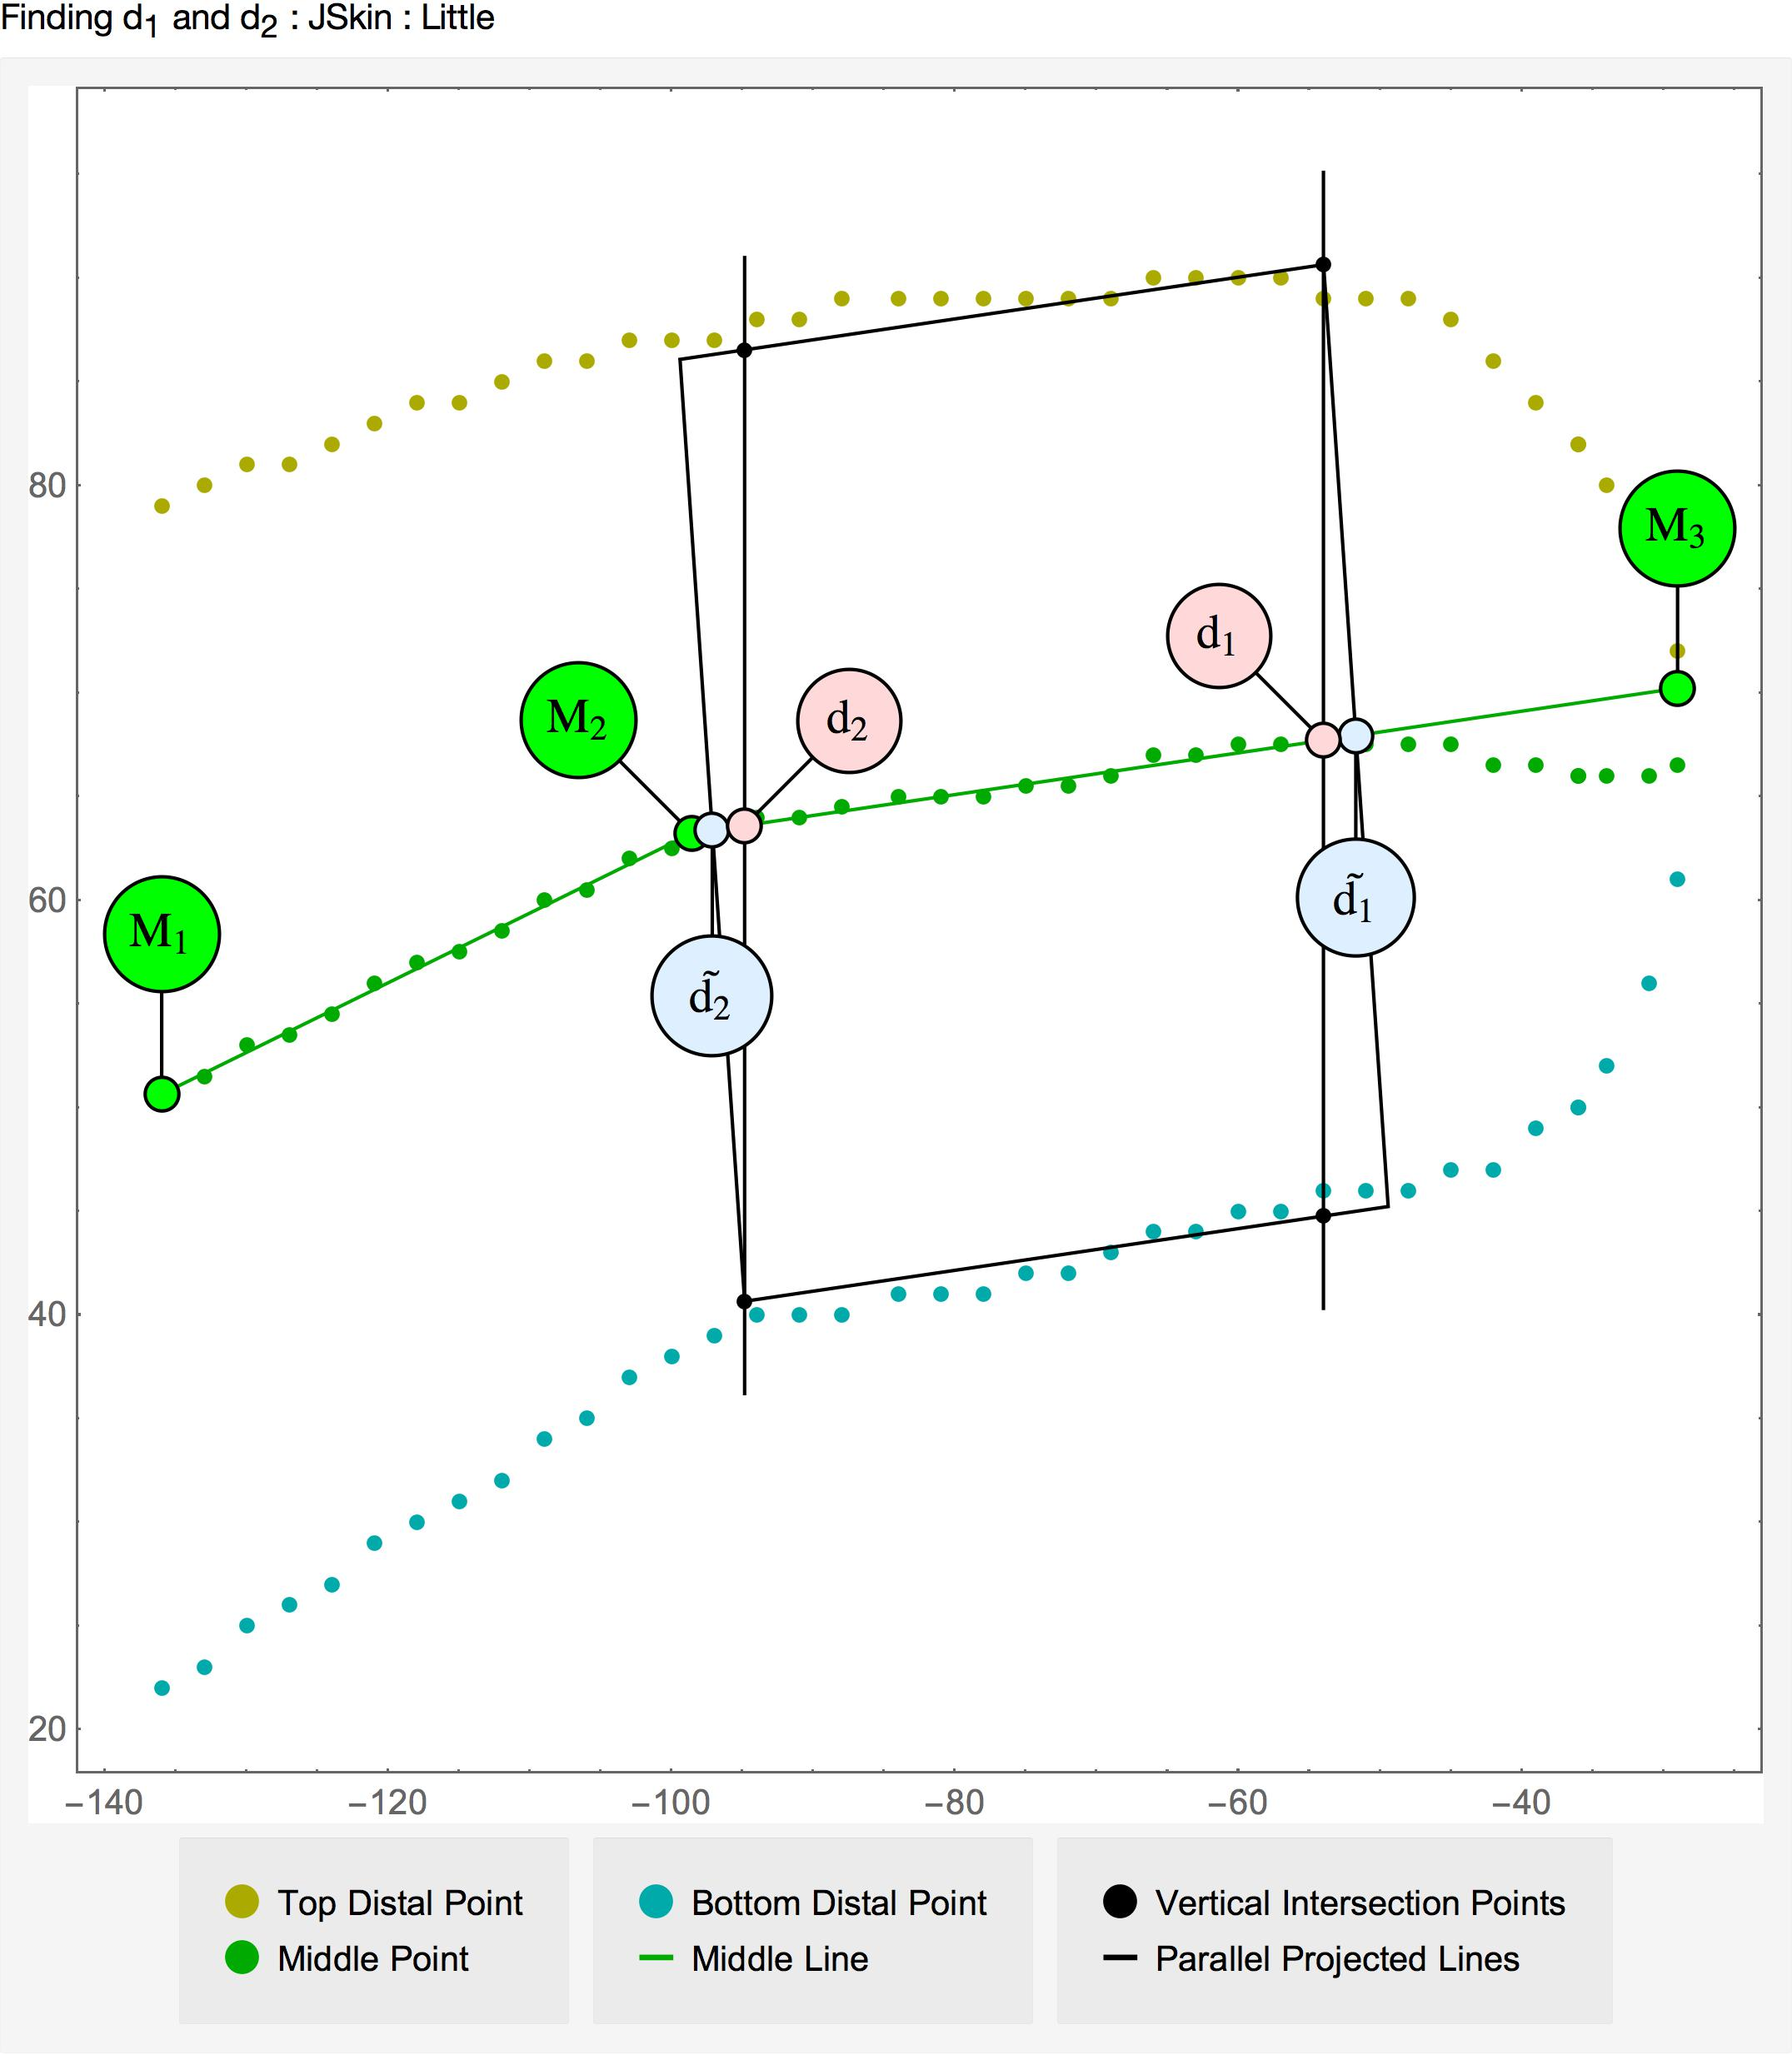
\includegraphics[width=0.45\textwidth, height=0.5\textwidth]{Chapter4/Figs/Model_FindingD1AndD2_JSkin_Little.jpg} &
    \parbox[b][0.5\textwidth][s]{0.55\textwidth}{
   \textbf{a) Determining $d_1$ \& $d_2$} --- We have a midline which is given as two points $M_2$ \& $M_3$; one somewhere on the digit ($M_2$), and the other at the tip ($M_3$). If the finger were straight in the frame, then $d_1=\tilde{d_1}$ and $d_2=\tilde{d_2}$ could easily be found by finding the points on that line. However, the fact that the digit can be presented at an angle means that the edge points vertically above and below the point on the midline may include part of the curved tip. This has the effect of making these midpoints diverge from the midline of the digit. This can be corrected by adjusting with half the gradient of the midline $\delta\:mid$ to the ratios. \begin{equation*}distance \:on \:line = (\frac{1}{2} + \left\lvert\frac{1}{2}\delta\:mid\right\lvert) w\end{equation*} \vfill
    } \\ 
    \parbox[b][0.5\textwidth][s]{0.45\textwidth}{
             \textbf{b) A New Midline Fit} --- We take the set of midline points, extract the subset which lies between $d_1$ and $d_2$, and then apply a straight line fit to these points. The origin is the fit evaluated at the $x$ component of $d_2$, and we determine an orientation $\theta$, which is $\arctan$ the gradient of the linear model. \vfill
        } &
        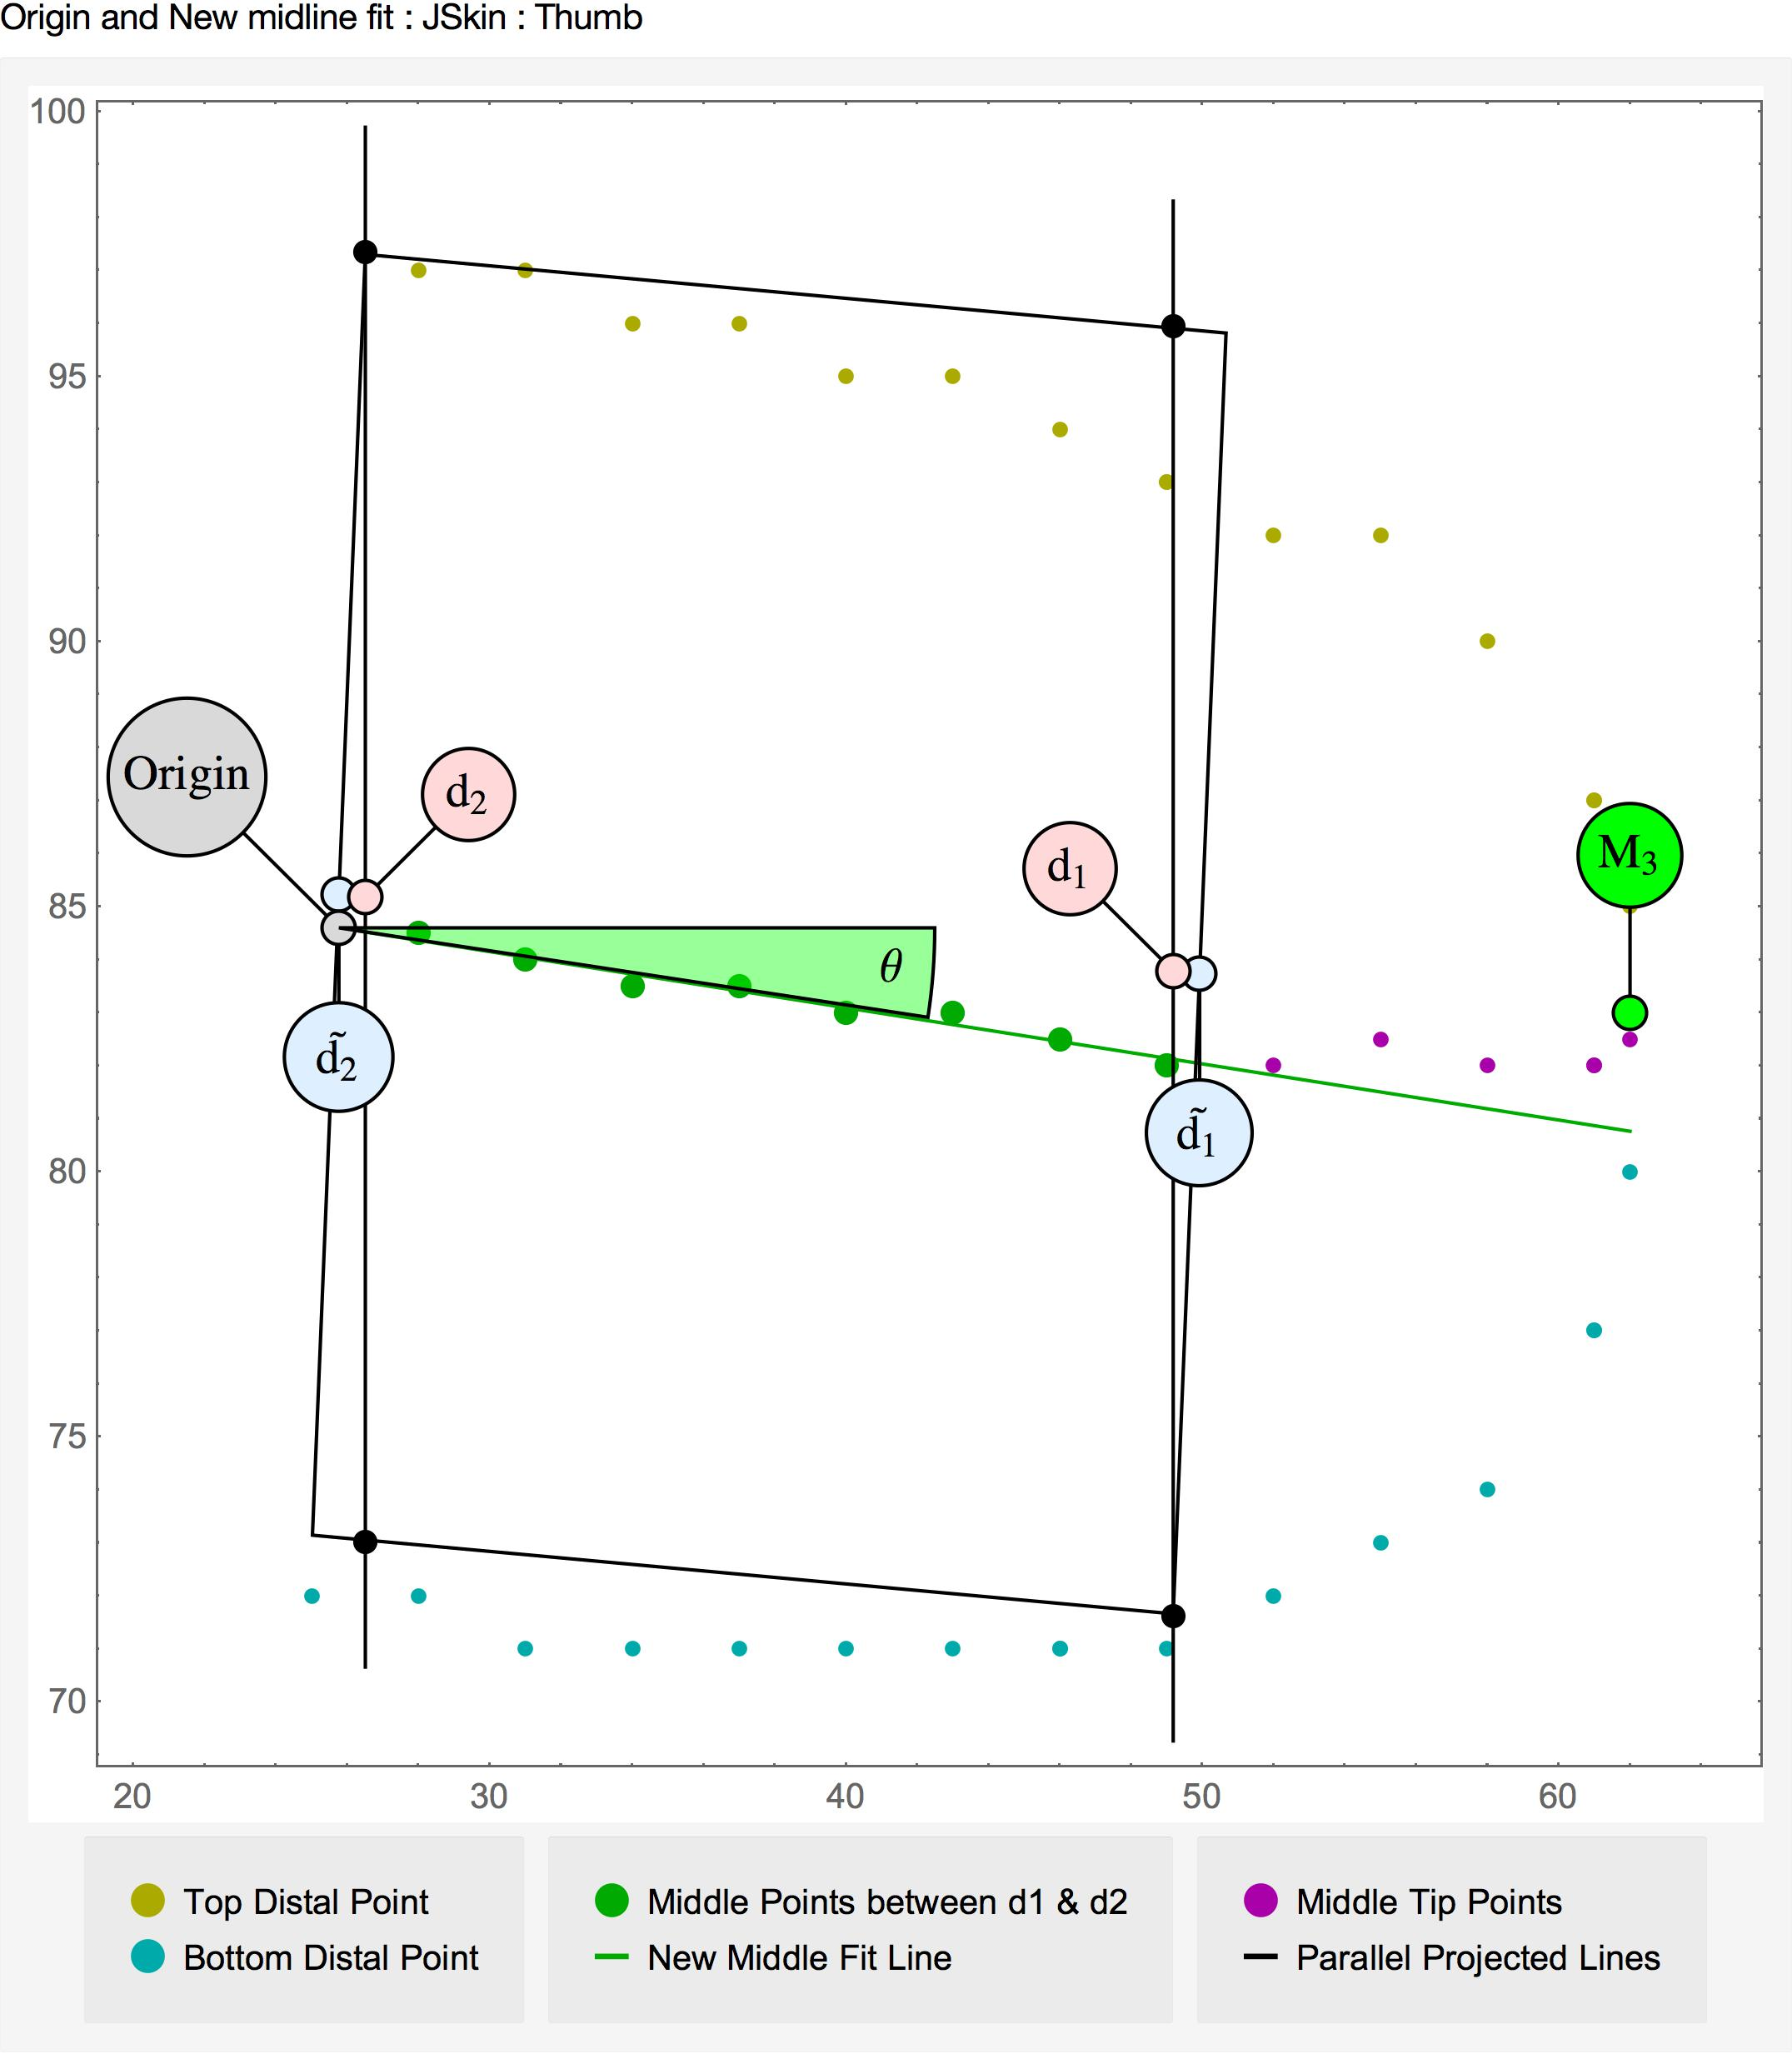
\includegraphics[width=0.55\textwidth, height=0.5\textwidth]{Chapter4/Figs/Model_Midline_JSkin_Thumb.jpg} 
    \\ 
   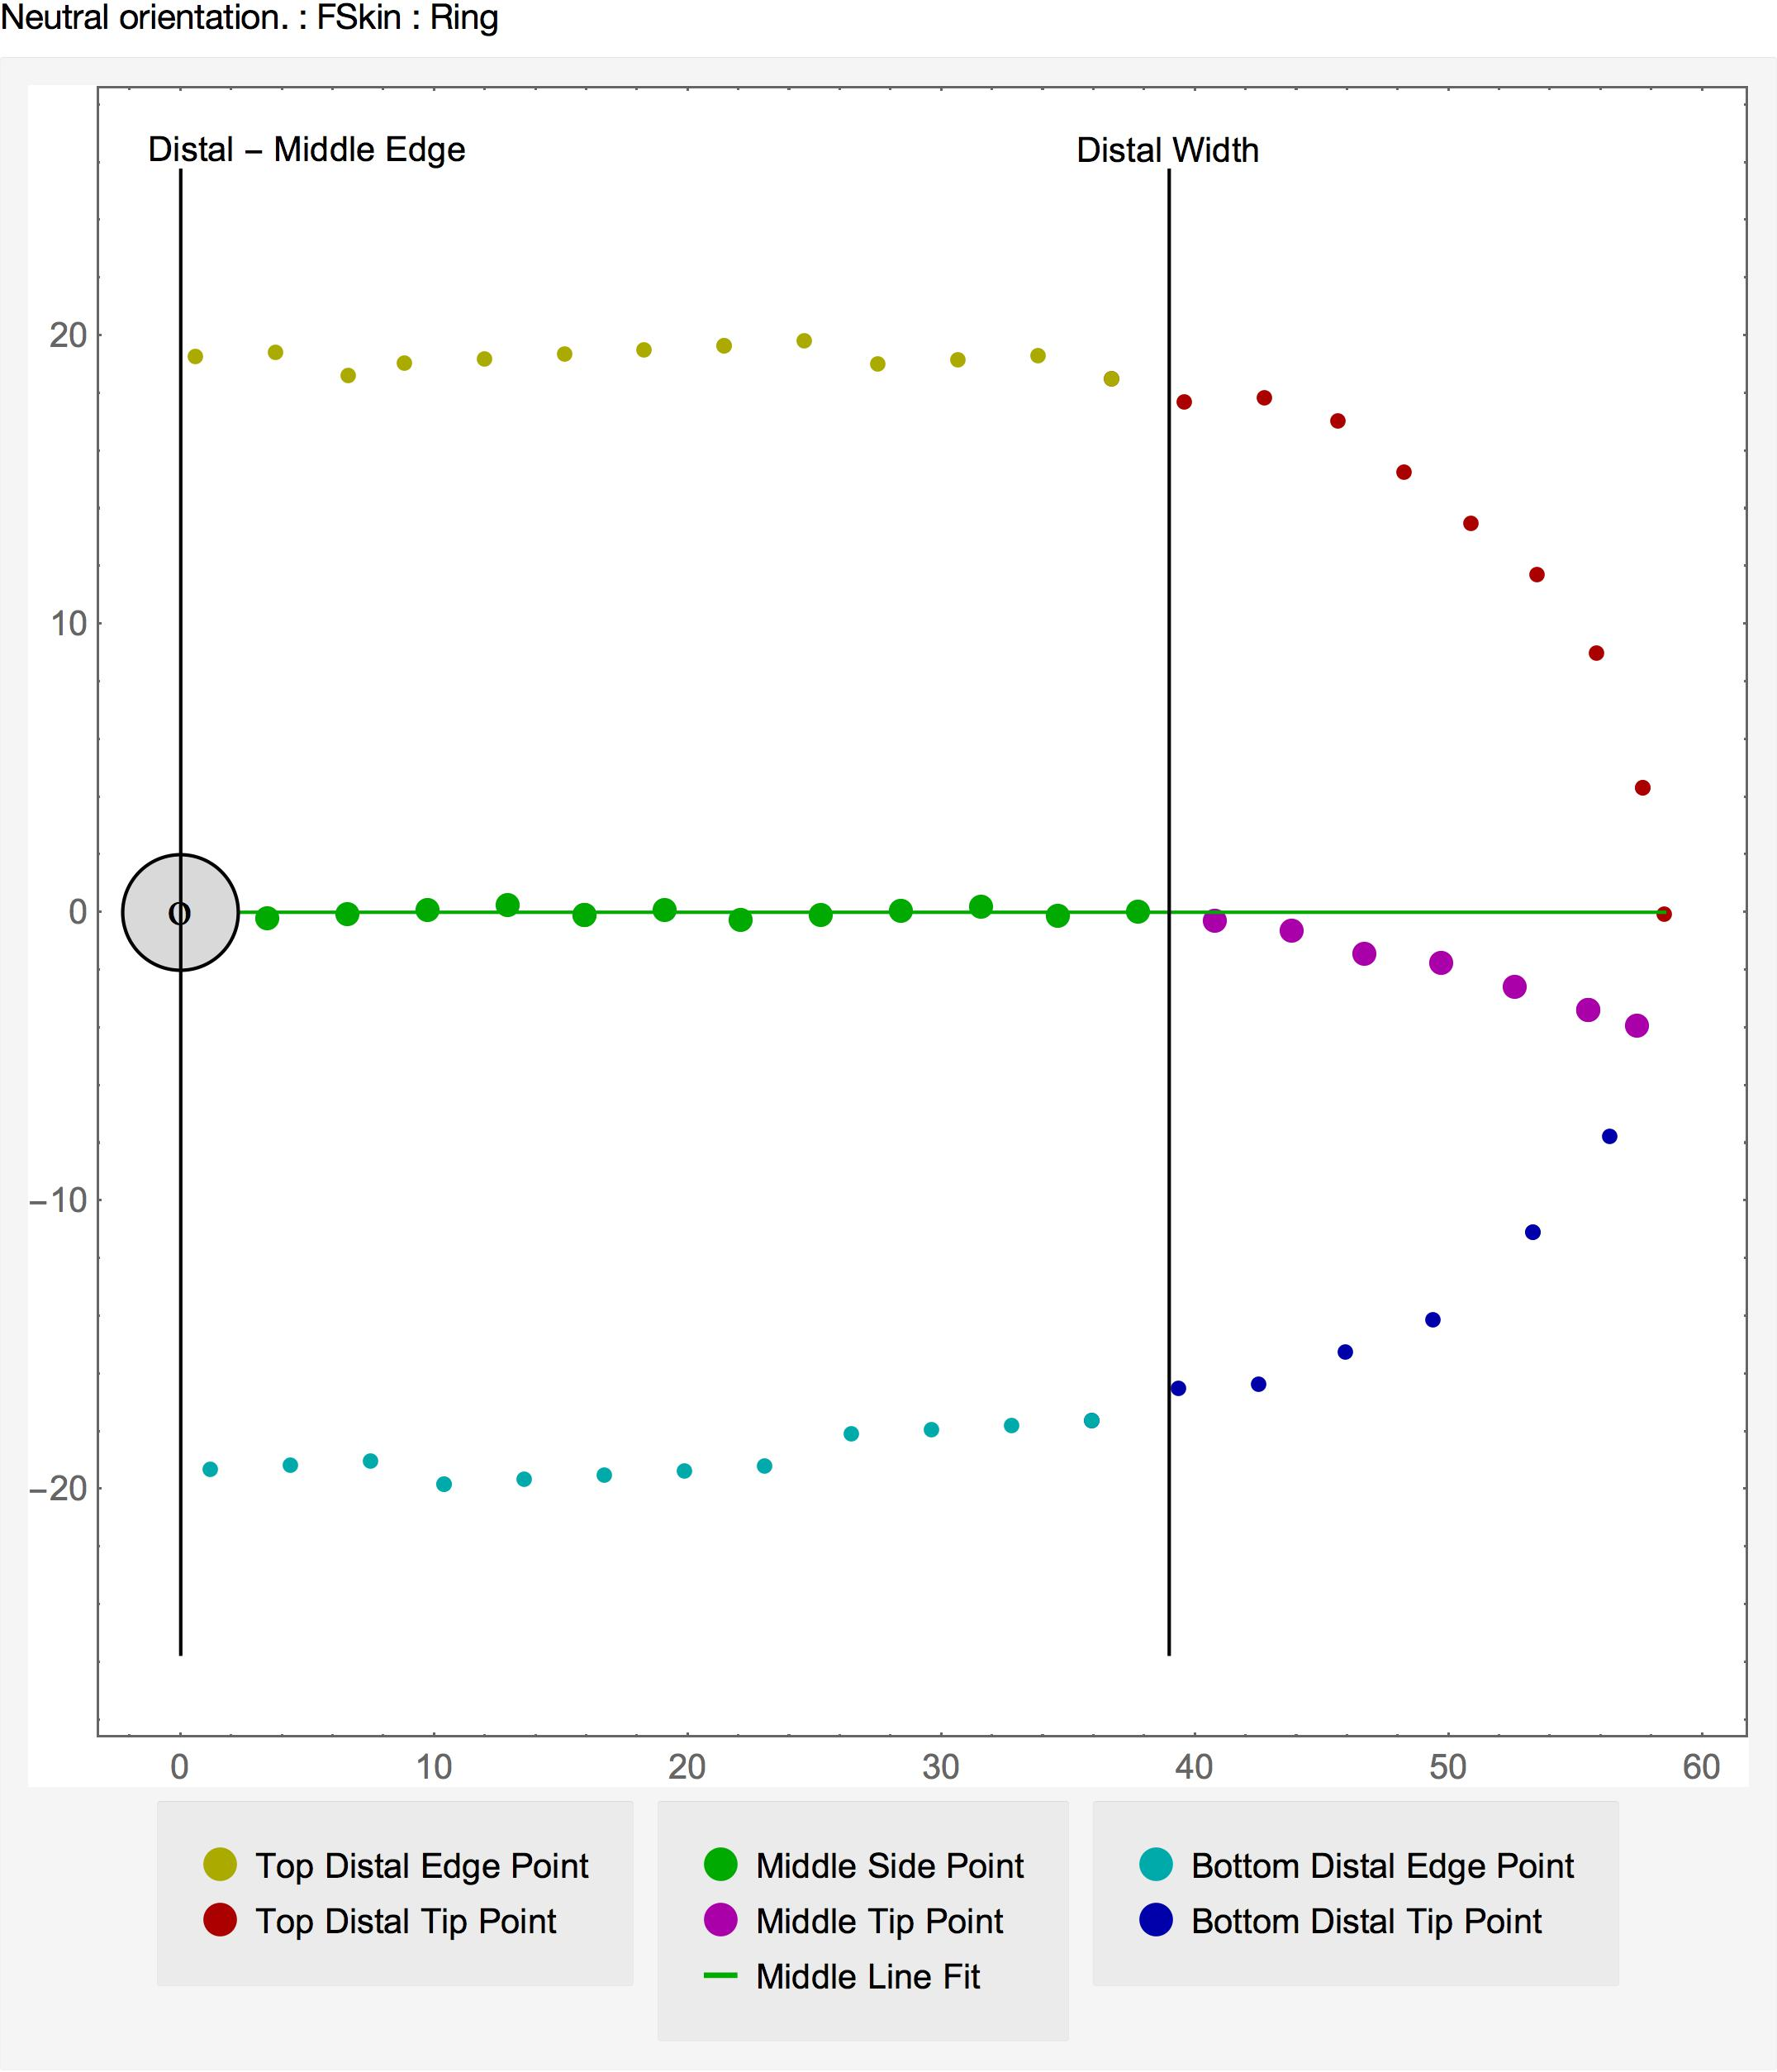
\includegraphics[width=0.45\textwidth, height=0.5\textwidth]{Chapter4/Figs/Model_NeutralCoords_FSkin_Ring.jpg} &
    \parbox[b][0.5\textwidth][s]{0.55\textwidth}{
         \textbf{c) Determine the Neutral Coordinates} --- We move all the points --- the top and bottom edges, and the midline points --- and we translate to the new origin. Then, we rotate by $-\theta$. This we call the "neutral co-ordinates", as the tip is aligned with its midaxis lying on the $x$ axis. These points are separated at one distal width from the tip; a Trapezian fit is applied to one set of points, and an Elliptical fit is applied to the other. As a refinement to this, although the linear fit is applied as in the Trapezian section, the algorithm then looks at the points beyond and before the one distal width region; if they're consistent with the fit, then they are considered still part of the straight edge. The Elliptical fit is applied as discussed previously. \vfill
    }
    \end{tabular}\\
    \phantomcaption
\end{figure}


\begin{figure}[p!]
\ContinuedFloat
\centering
\begin{minipage}[t]{1\textwidth}
\begin{wrapfigure}{l}{0.5\textwidth}
  \begin{center}
    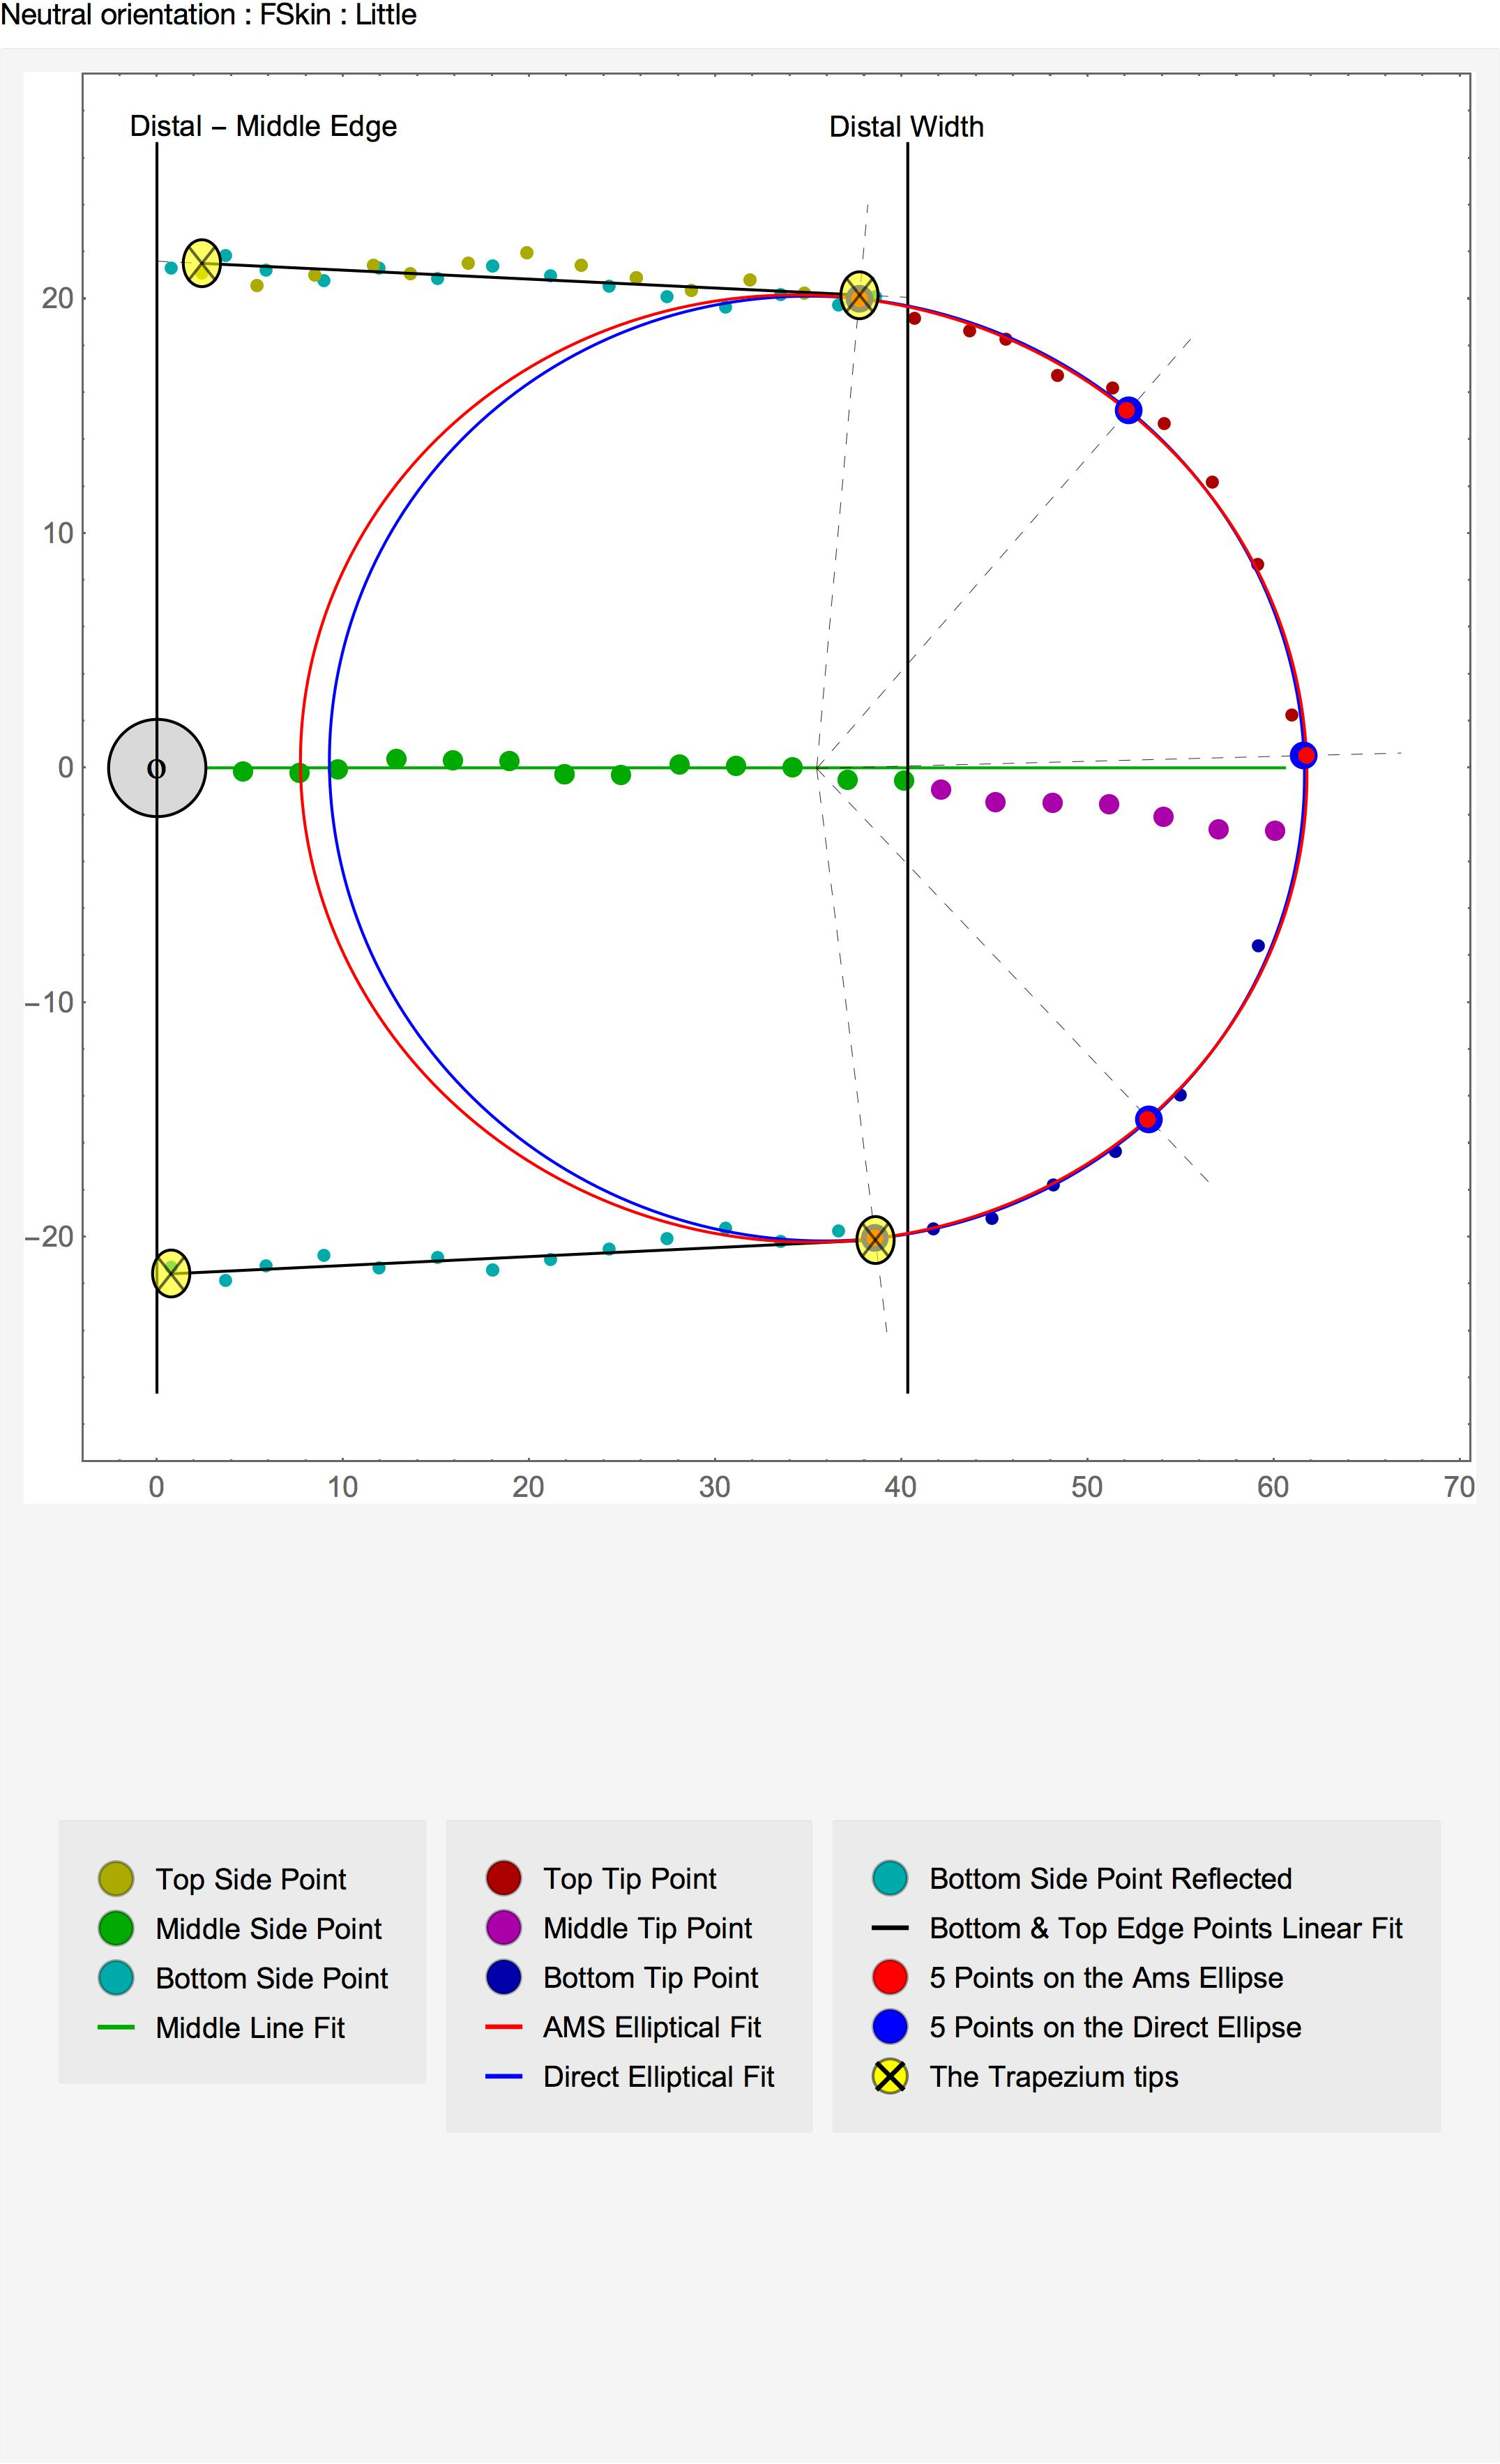
\includegraphics[width=0.5\textwidth]{Chapter4/Figs/Model_ShapeFitting_FSkin_Little.jpg}
  \end{center}
  \phantomcaption
\end{wrapfigure}
         \textbf{d) Fitting the Shapes} --- The comparison between the elliptical fit methods is done by looking at the distance from the front two points on the trapezium to the edge of the ellipse, and the best of these is chosen. Unfortunately, this is often not sufficient to make the ellipse join with the trapezium exactly because further on in the algorithm, these shapes will be used to perform a mask; we want to avoid introducing artefacts which could be interpreted as features. So, we wish to remove these discontinuous intersections between the ellipse and the trapezium. In order to do this, we choose three points on the Elliptical fit and the two front points of the trapezium, thereby making a set of five points, and we pass these through the direct Elliptical fit algorithm. It should be noted that five points is what is required to completely define an ellipse; there is only one ellipse which will pass through five points.
    \end{minipage}
    \subfloat{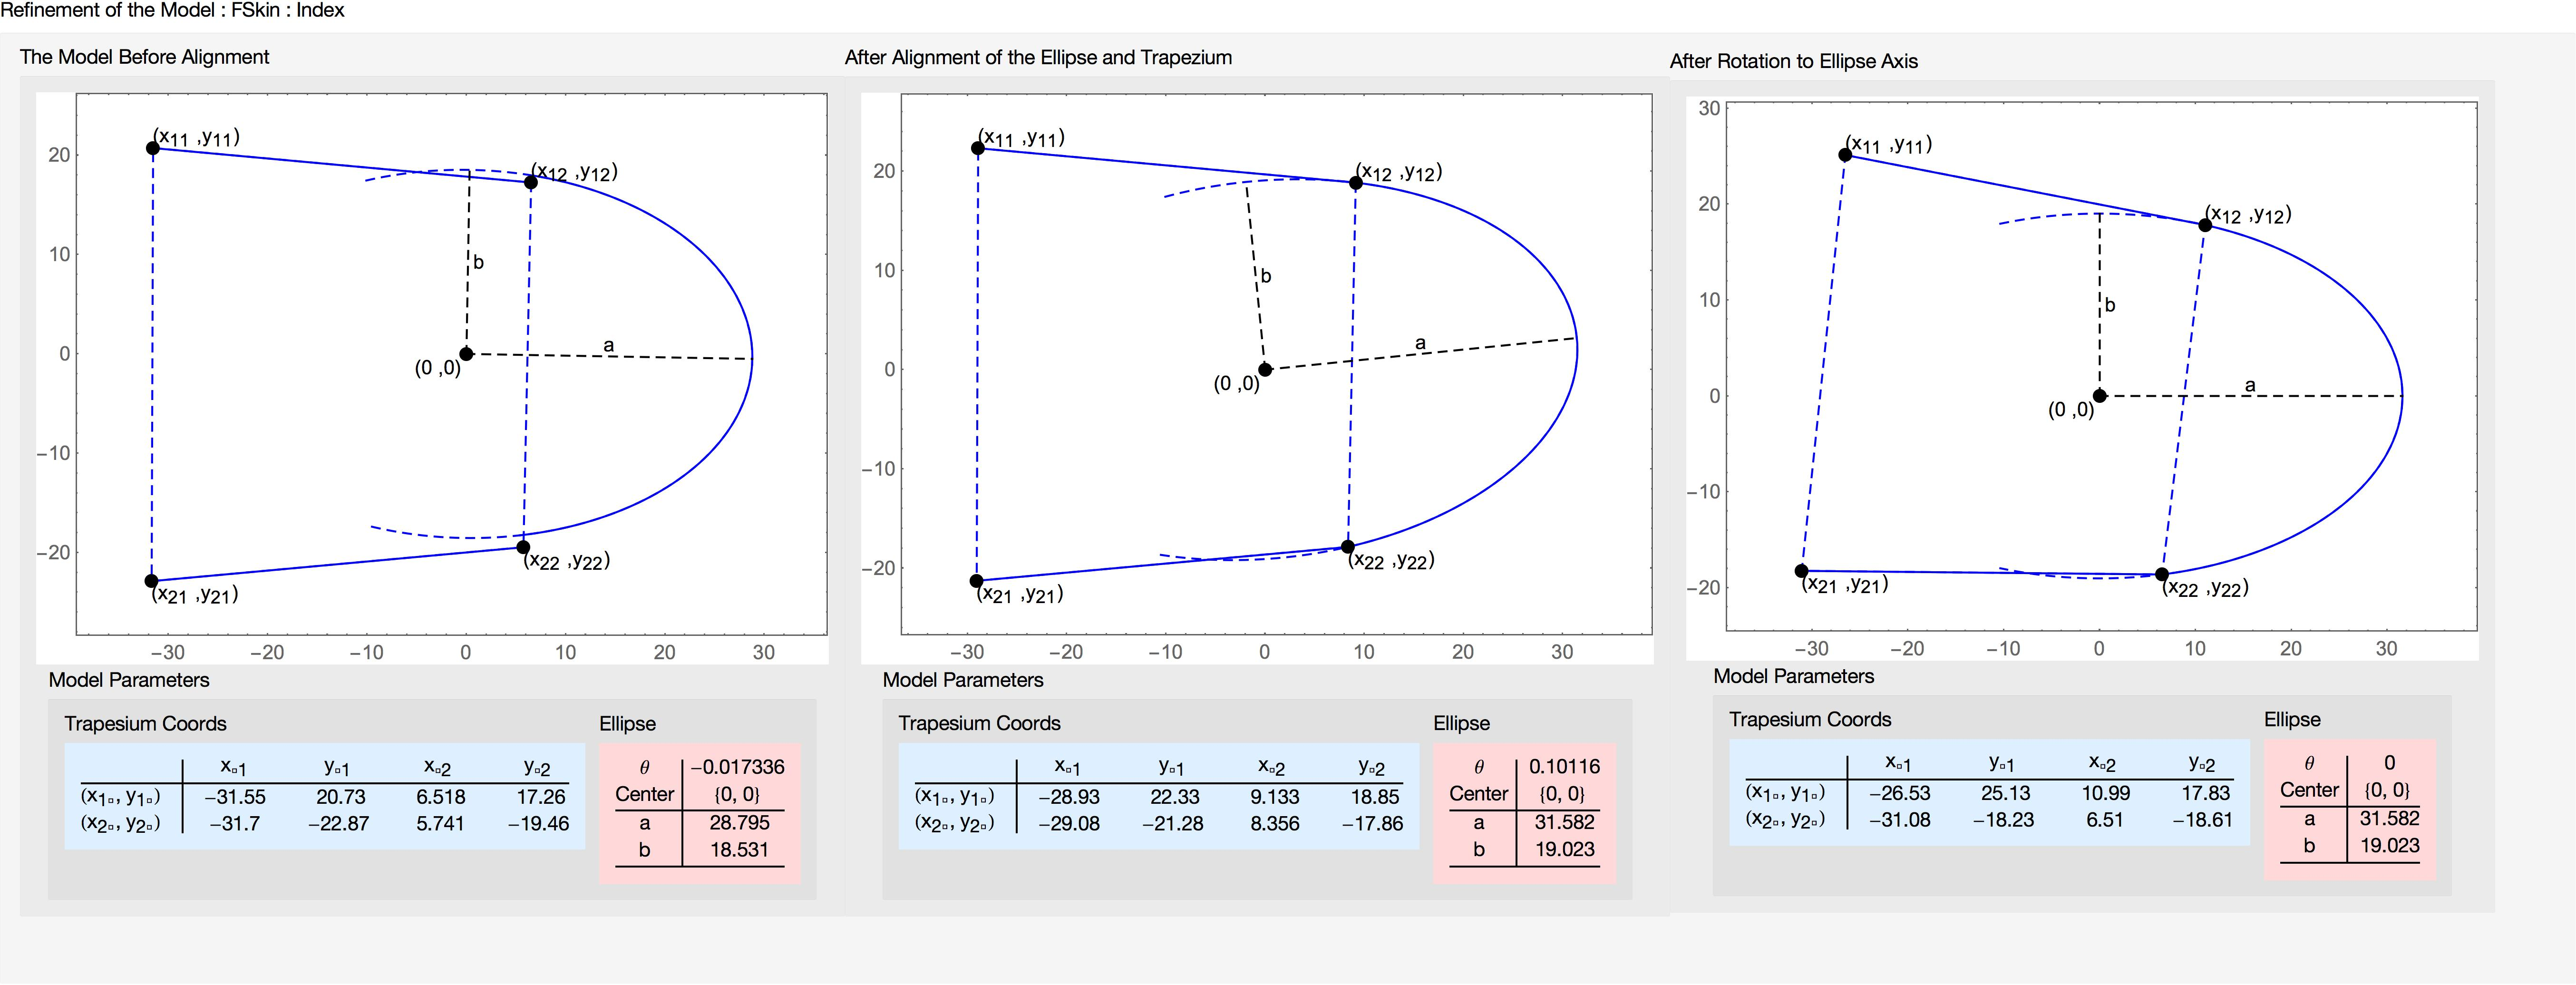
\includegraphics[width=0.99\textwidth]{Chapter4/Figs/Model_Finalizing_FSkin_Index.jpg}}\\
    \begin{minipage}{0.95\textwidth}
         \textbf{e) Finalizing the Model} --- The coordinates for the ellipse and the trapezian are adjusted so that the origin is at the center of the ellipse, and the ellipse has zero rotation. The reason for this is that it makes calculating the distance from the edges of the ellipse easier. So, now when we apply the model to the image, all that's required is a position --- which is the position of the center of the ellipse --- and an orientation about that position. 
    \end{minipage}
    \caption{The Fingertip Model Algorithm.}\label{fig:ModelingFingertip}
\end{figure}

Having determined a measure of the width of the distal portion of the fingertip allows for a more robust model of the fingertip to be determined. This is because the measurement of the distal width is far more reliable than the distal length which has so far been determined, as the distal length has been found by evaluating where the "kink" of the midline points lies. For example, if the distal joint is unflexed, the knuckle portion will be overlooked entirely, as seen in Figure \ref{fig:ParallelFit}. It turns out that the anatomical ratios (Section \ref{sec:FingertipModel}) are a far more reliable method of determining the distal length.

From the kink fit, we have a midline, which is specified by three points. We now determine two points on this line, which are $\frac{1}{2}$ the distal width ($d_1$) and $1\frac{1}{2}$ the distal width from the tip ($d_2$). So the midline point that lies between the two points can now be taken to correspond to the straight-edged section of the distal portion of the finger. These points are passed to the Trapezian Fit method (\ref{sec:TrapezianFit}), and the points which lie between the tip and the point half the distal width from the tip are passed to the Elliptical Fit (\ref{sec:EllipticalFitMethod}). The ellipse is adjusted to correspond with the two near vertices of the Trapezian; the result can be seen in Figure \ref{fig:ModelingFingertip}.

To illustrate the model, we can overlay the model on its source image in the original orientation and position. This shows that the application of the model actually only requires a position and orientation, because we assume that the camera is positioned such that the digit presents at the same scale when in contact with a surface throughout the frame; we're not accounting for perspective effects in this simple application.

The model can be seen overlayed on the selection of digits for three individuals in Figure \ref{fig:FingertipModelResult}.

\begin{figure}[h!]
  \centering
    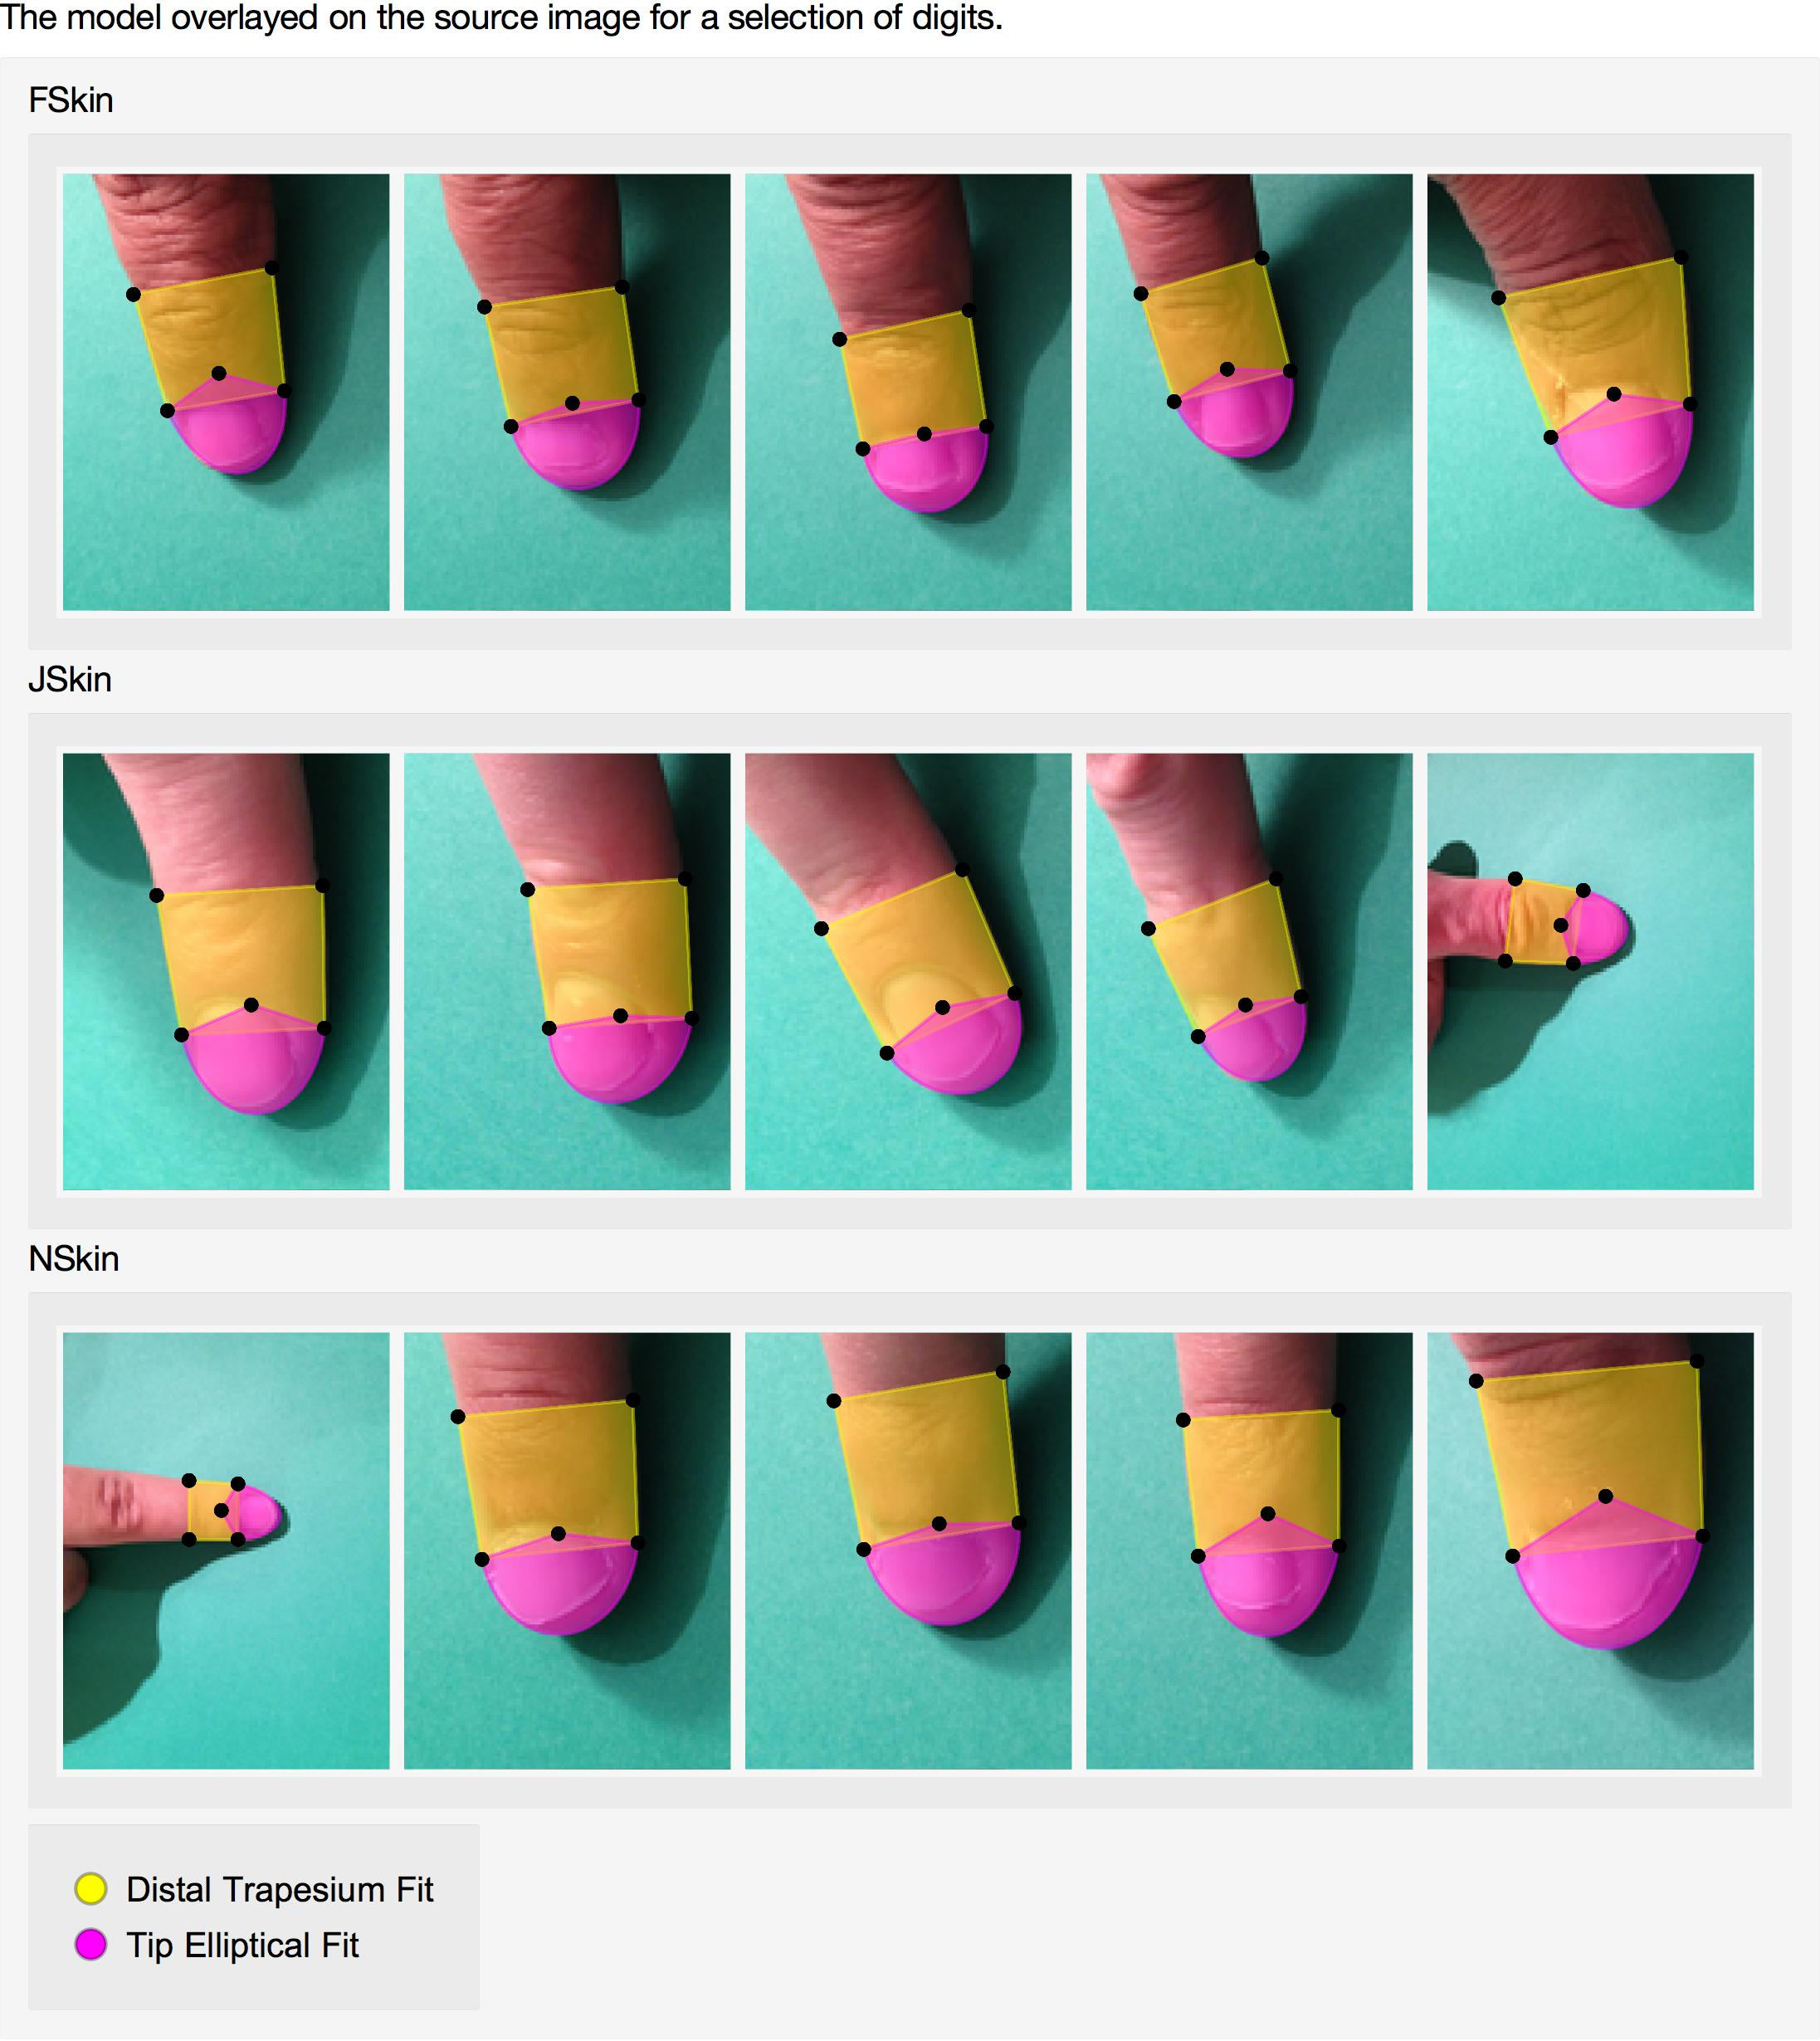
\includegraphics[width=0.83\textwidth]{Chapter4/Figs/Model_Overlayed.jpg}
    \caption{The models overlayed on the source images.}\label{fig:FingertipModelResult}
\end{figure}

\begin{sidewaysfigure}[h!]
  \centering
    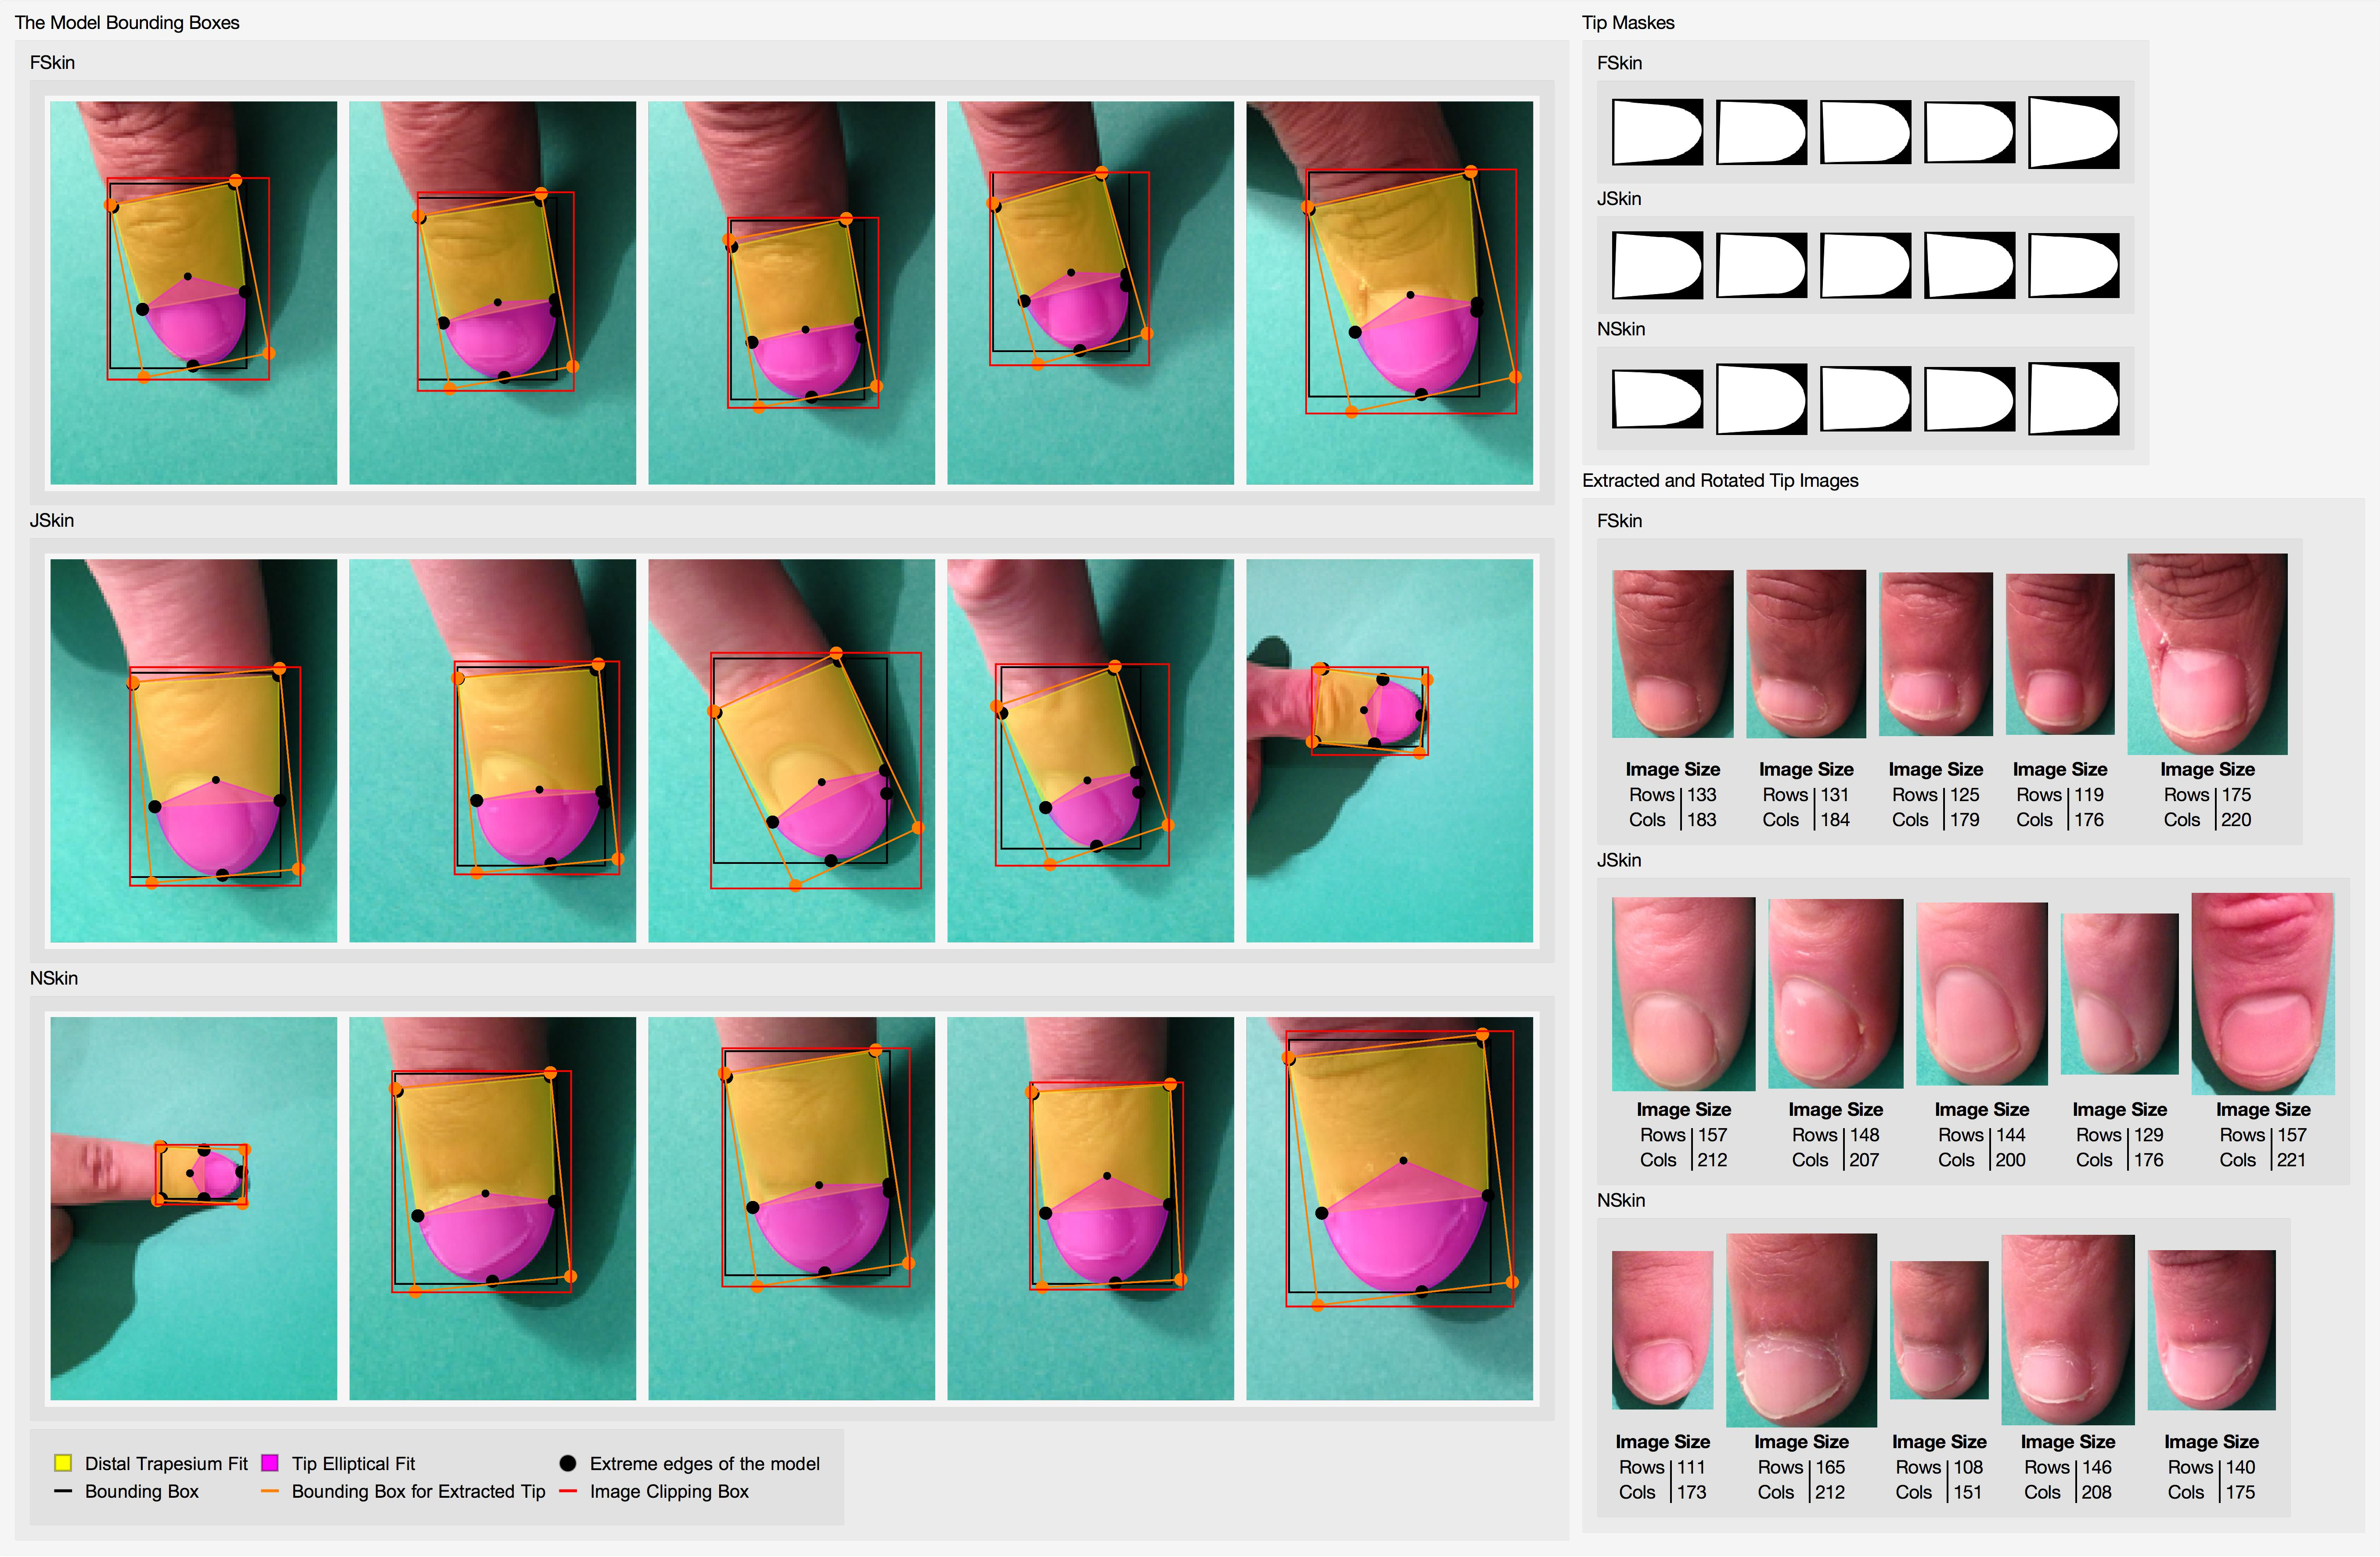
\includegraphics[width=0.95\textwidth]{Chapter4/Figs/Model_Overlayed_Boundary_with_Tips.jpg}
    \caption{The models and model boundaries overlayed on the source images. With tip masks and extracted tip images.}\label{fig:ModelOverlayedBoundaryWithTips}
\end{sidewaysfigure}


\clearpage
\section{Dynamic Tracking}\label{sec:DynamicTracking}
The main purpose of the dynamic tracking algorithm is to categorize the motion of the digit in the frame as "rapid motion," "smooth motion," and "in contact with a surface."

\begin{itemize}
\item \textbf{Rapid motion} --- When the digit is being moved into the frame, or is moving rapidly across the frame, or when the camera is being put into position, it is pointless to attempt to detect a fingertip as this information will quickly become irrelevant. Standard motion detection library routines can be used here on the unaltered video feed. When these algorithms detect motion above a certain threshold, the algorithm does nothing and waits for the motion detected to fall below this threshold.
\item \textbf{Smooth motion} --- Smooth motion is when the digit is being moved in a controlled manner within the frame. When the digit is moving in such a way, it is reasonable to assume that a finger press is imminent. The algorithm takes a frame in the small scale space and processes it into a pixel-categorized image as in section \ref{sec:QuaternaryPixelClassification}. The frame orientation and digit tip selection are found as in sections \ref{sec:FindingTheFrameOrientation} and \ref{sec:FindingTheEndOfTheFingerShape}, and then a Filament fill of only the tip is performed similar to sections \ref{sec:FilamentFill} and \ref{sec:FilamentFillTheFinger}, but now with the Filament fill path being shortened to the length of the distal section in the model. The position and orientation for the model are obtained using the Force Analogue Shape Detection algorithm outlined below, in section \ref{sec:ForceAnalogue}. The algorithm continues tracking until the change in the position of the tip between successive frames falls below a threshold, at which point the algorithm decides that the digit is likely in contact with a surface, and control passes to the "in contact with a surface" part of the algorithm.
\item \textbf{In contact with a surface (ICWaS)} --- When the tip of the digit is relatively immobile, the digit is likely in contact with a surface; we now want to observe the blood flow. The frame is now captured in the medium space, and is cropped to the edges of the model in its current position and orientation. The cropped image is put into the skin color space, and a gradient filter is applied to the grayscale channel. If this is the first iteration, this gradient-filtered image is stored; if it is a subsequent iteration, this gradient filter is compared with the first and an alignment transform is found between the current frame and the first frame. To improve the accuracy and avoid the algorithm being distracted by movements at the edge of the digit, the gradient-filtered images are masked with the model, which removes edge-related gradient features, focusing the algorithm on the nail, which is stable during a finger press. The transform is applied to the two chromatic channels, which aligns the images, and the difference is found between successive frames; this gives us the blood flow. 
\end{itemize}

\subsection{Rapid Motion Tracking}\label{sec:RapidMotionTracking}
Before any fingertip tracking is performed, the algorithm checks to see if the digit is still in motion. This is done by first taking the difference between subsequent grayscaled frames from the raw video feed using OpenCV's 'absdiff' method. To account for changes in lighting and contrast, a binary threshold is applied to the frames, after which an erosion operation (the 'erode' method) is performed to further reduce artifacts and false positives. If the number of changes in the image is above a given threshold, then the digit is considered to be in rapid motion.


\subsection{Smooth Motion Tracking}\label{sec:SmoothMotionTracking}

The find-tip algorithm (section \ref{sec:FindingTheEndOfTheFingerShape}) gives us a path which we know lies on a digit. This path, however, is not necessarily particularly well-aligned with the axis of the digit. For this reason, we don't ask for a shortened path from the tip to $1 \frac{1}{2}$ distal widths along that path; such a path might actually end closer to the tip than desired, as the path isn't necessarily along the axis. To account for this, we ask for two distal widths from the tip. 

The next problem to be addressed results from the operation of the Filament fill method; because the digit isn't necessarily presented perpendicularly to the frame edge and the Filament fill algorithm finds points perpendicular to the frame edge, we adjust by half the gradient of the path, similarly to the method used in the fingertip model algorithm illustrated in Figure \ref{fig:ModelingFingertip}. So, Filament fill is run along the find-tip path from the tip to a distance of $(2+\left\lvert\frac{1}{2}\delta path\right\lvert)w$ from the tip. This gives us three sets of points: the top, middle and bottom edges, which definitely include points relating to the tip of the digit.

Now we refine these points; because we know the orientation of the frame, we can determine which points correspond to the top edge of the digit, and which points correspond to the bottom. We now put them into standard orientation as in steps a and b in Figure \ref{fig:ModelingFingertip}. 

We now need to find points on the model which would ideally correspond with the points found by Filament fill in the image. First, we need to obtain a reasonably good measure of the orientation of the digit; given that we have midline points on the digit which reasonably correspond to the distal segment, a linear fit to the middle $\frac{2}{3}$ of these points provides a good measure of the orientation with little computational cost. Rather than reorientating the image points to a neutral coordinates, we rotate the model to correspond with the image coordinates. This is easily achieved as the model is centered on the ellipse, and so involves a rotation of the four points of the trapezian and adding the rotation to the ellipse's orientation.

In the model's new orientation, we find the furthest point on the model in the $x$ axis. (It should be noted that this is not necessarily what we would refer to as the "tip" of the digit.) We assume that this point on the model corresponds to the first point in the midline set of points; the Filament fill follows the path from the tip back to the frame edge, so the first point in the midline should be the tip. So, we create a set of $x$ axis coordinates where the first midline point corresponds with the furthest point on the model in the $x$ axis. We do this because the Filament fill divides up the shape vertically in a relatively regular fashion, so we are dividing up the model in the way that we would expect Filament fill to if the model were an image. This allows us to put points on the model and points in the image into a $1:1$ correspondence. So although the fingertip model is a relatively arbitrary geometric shape, the regularity of the Filament fill method allows us to use a force analogue shape detection algorithm as outlined previously (section \ref{sec:ForceAnalogue}).

\begin{figure}[h!]
  \centering
    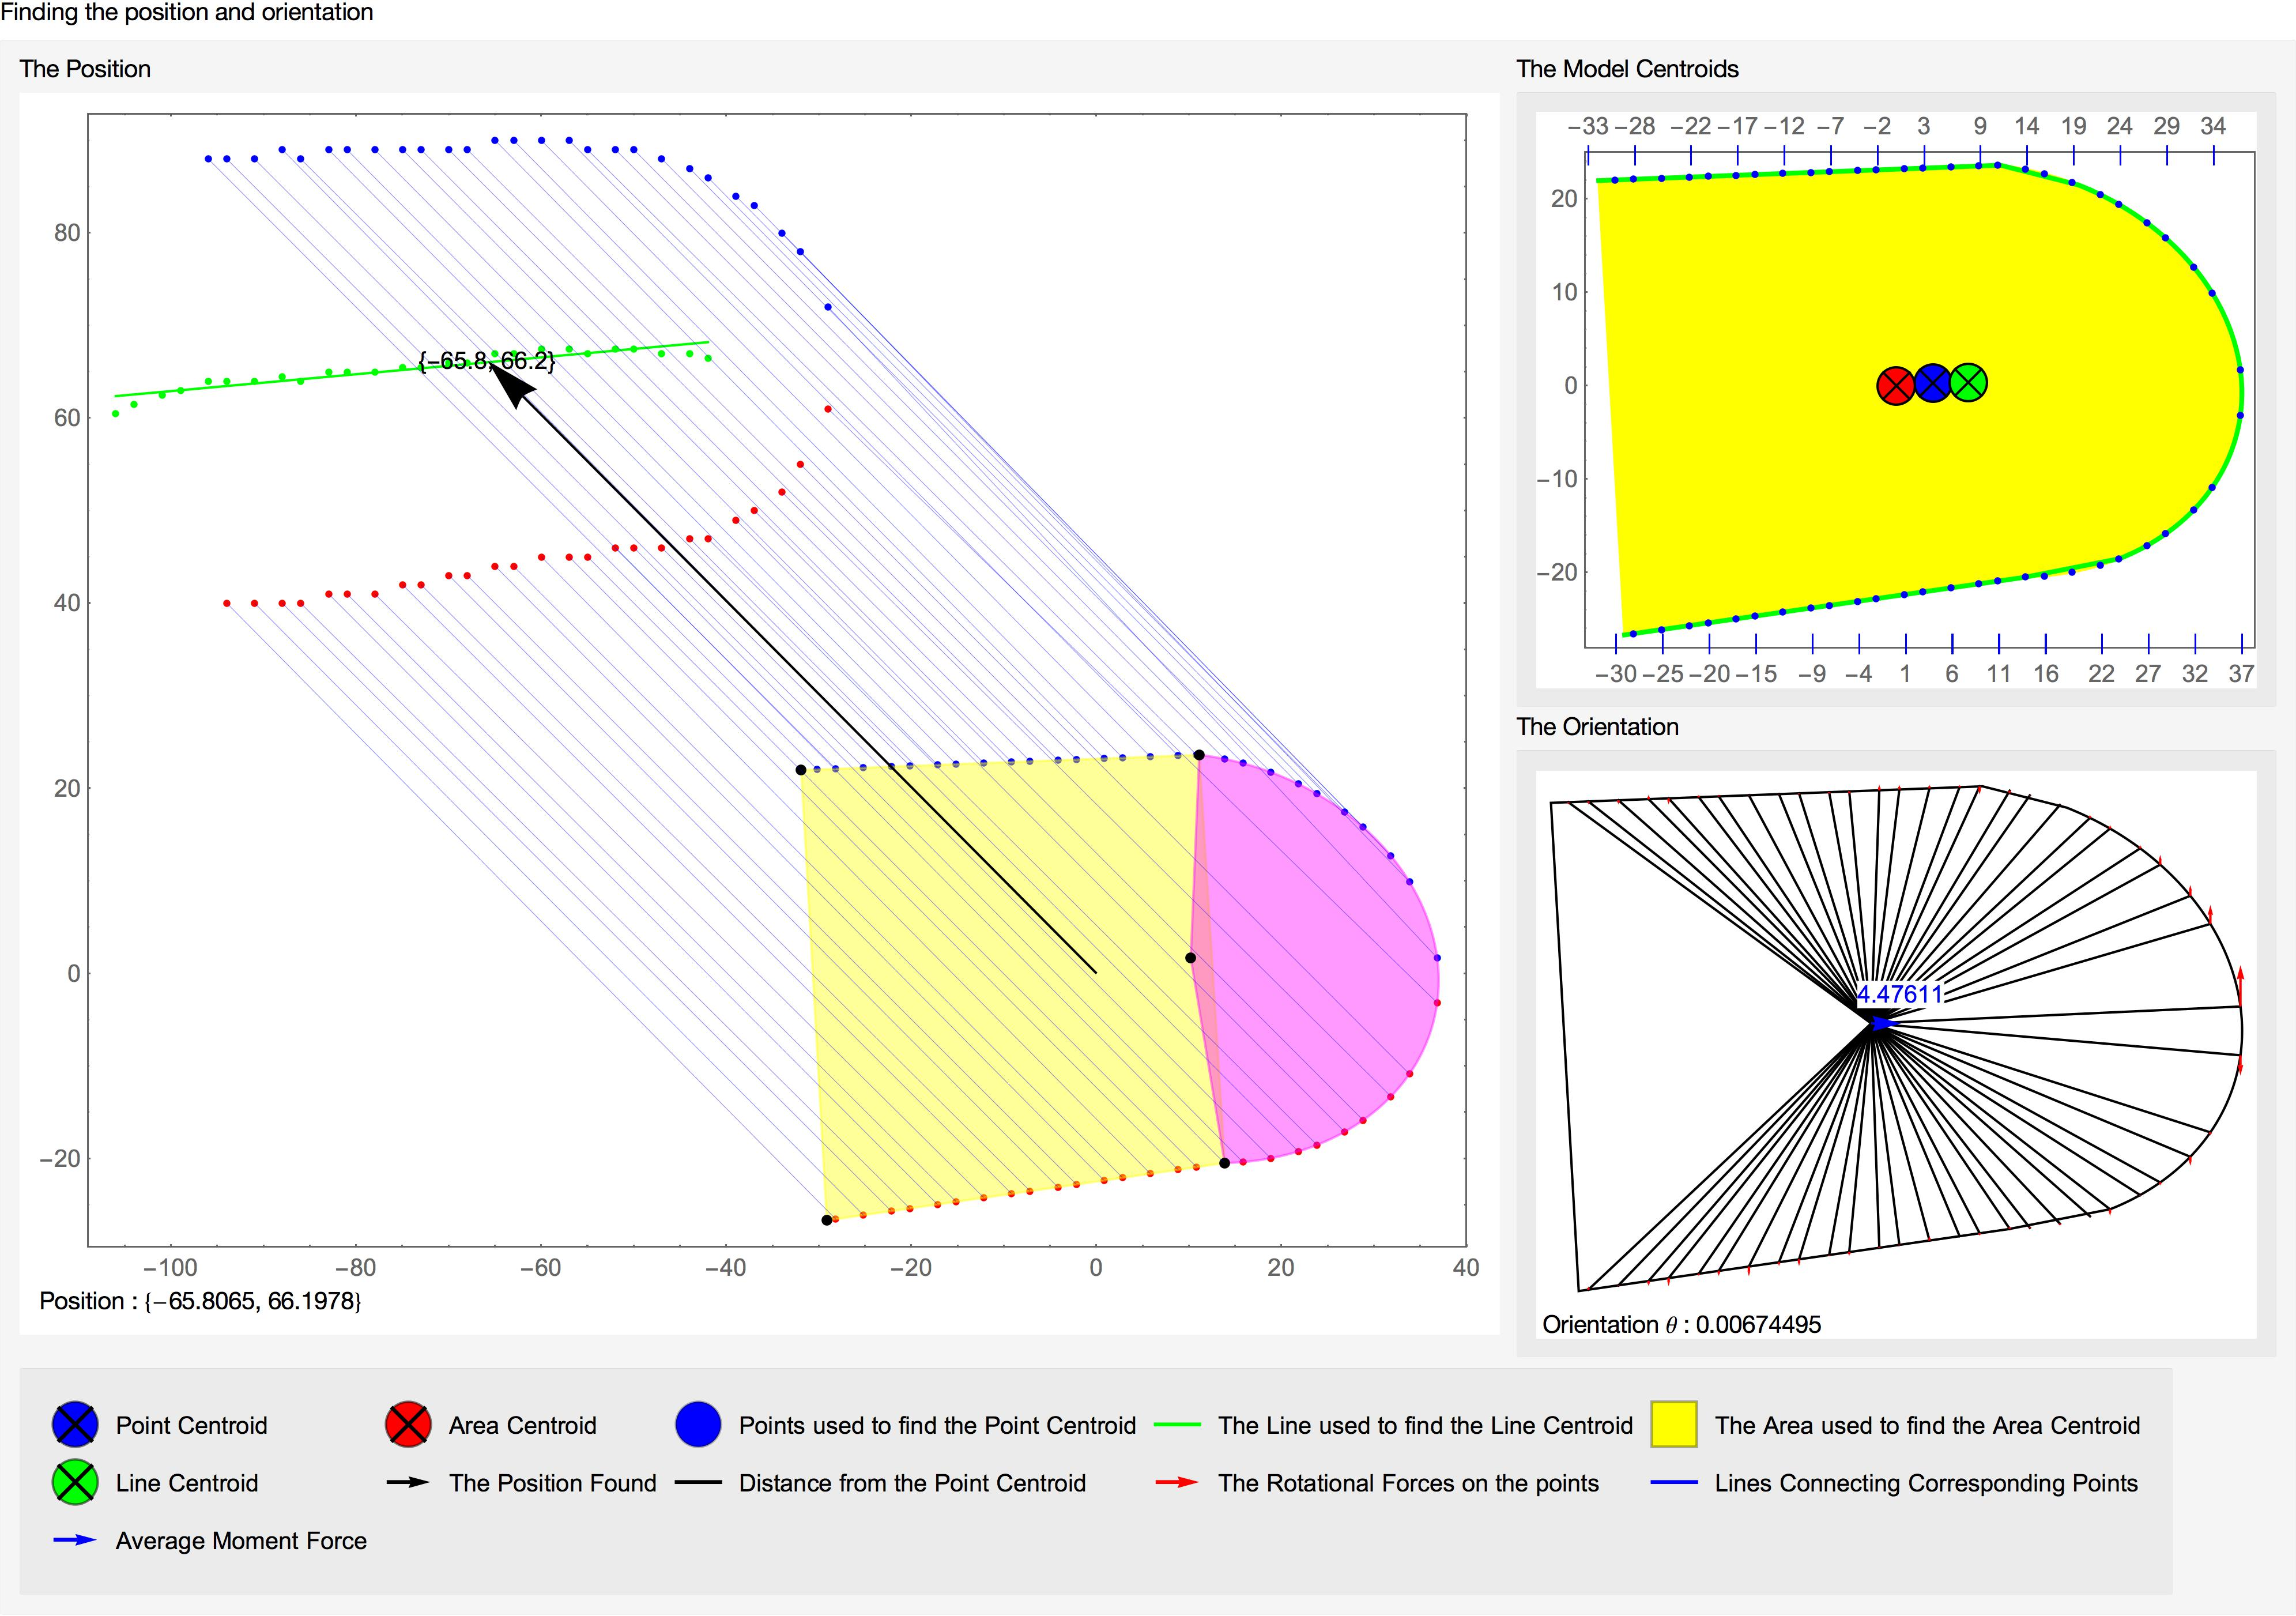
\includegraphics[width=0.95\textwidth]{Chapter4/Figs/Model_Centroids_With_Pos_Orientation.jpg}
    \caption{Finding the Position and Orientation of the Tip. A side-effect of the pre-alignment of the model means that, almost always,  the change in the orientation from the force analogue shape detection algorithm is negligible. }\label{fig:PositionAndOrientation}
\end{figure}

A side-effect of the pre-alignment of the model means that --- almost always --- the change in the orientation from the force analogue shape detection algorithm is negligible.

The dependence of the distribution of points around the perimeter of the model is dependant on the orientation of the digit in the image. This means that the point centroid is not predictable, and so a shape-based centroid is required in the modeling stage \ref{fig:PositionAndOrientation}. The Filament fill point distribution favors the top and bottom edges of the digit over the points on the tip itself, making a perimeter centroid unfavorable. For these reasons, the fingertip model is centered on the model's area centroid.

\begin{figure}[h!]
  \centering
    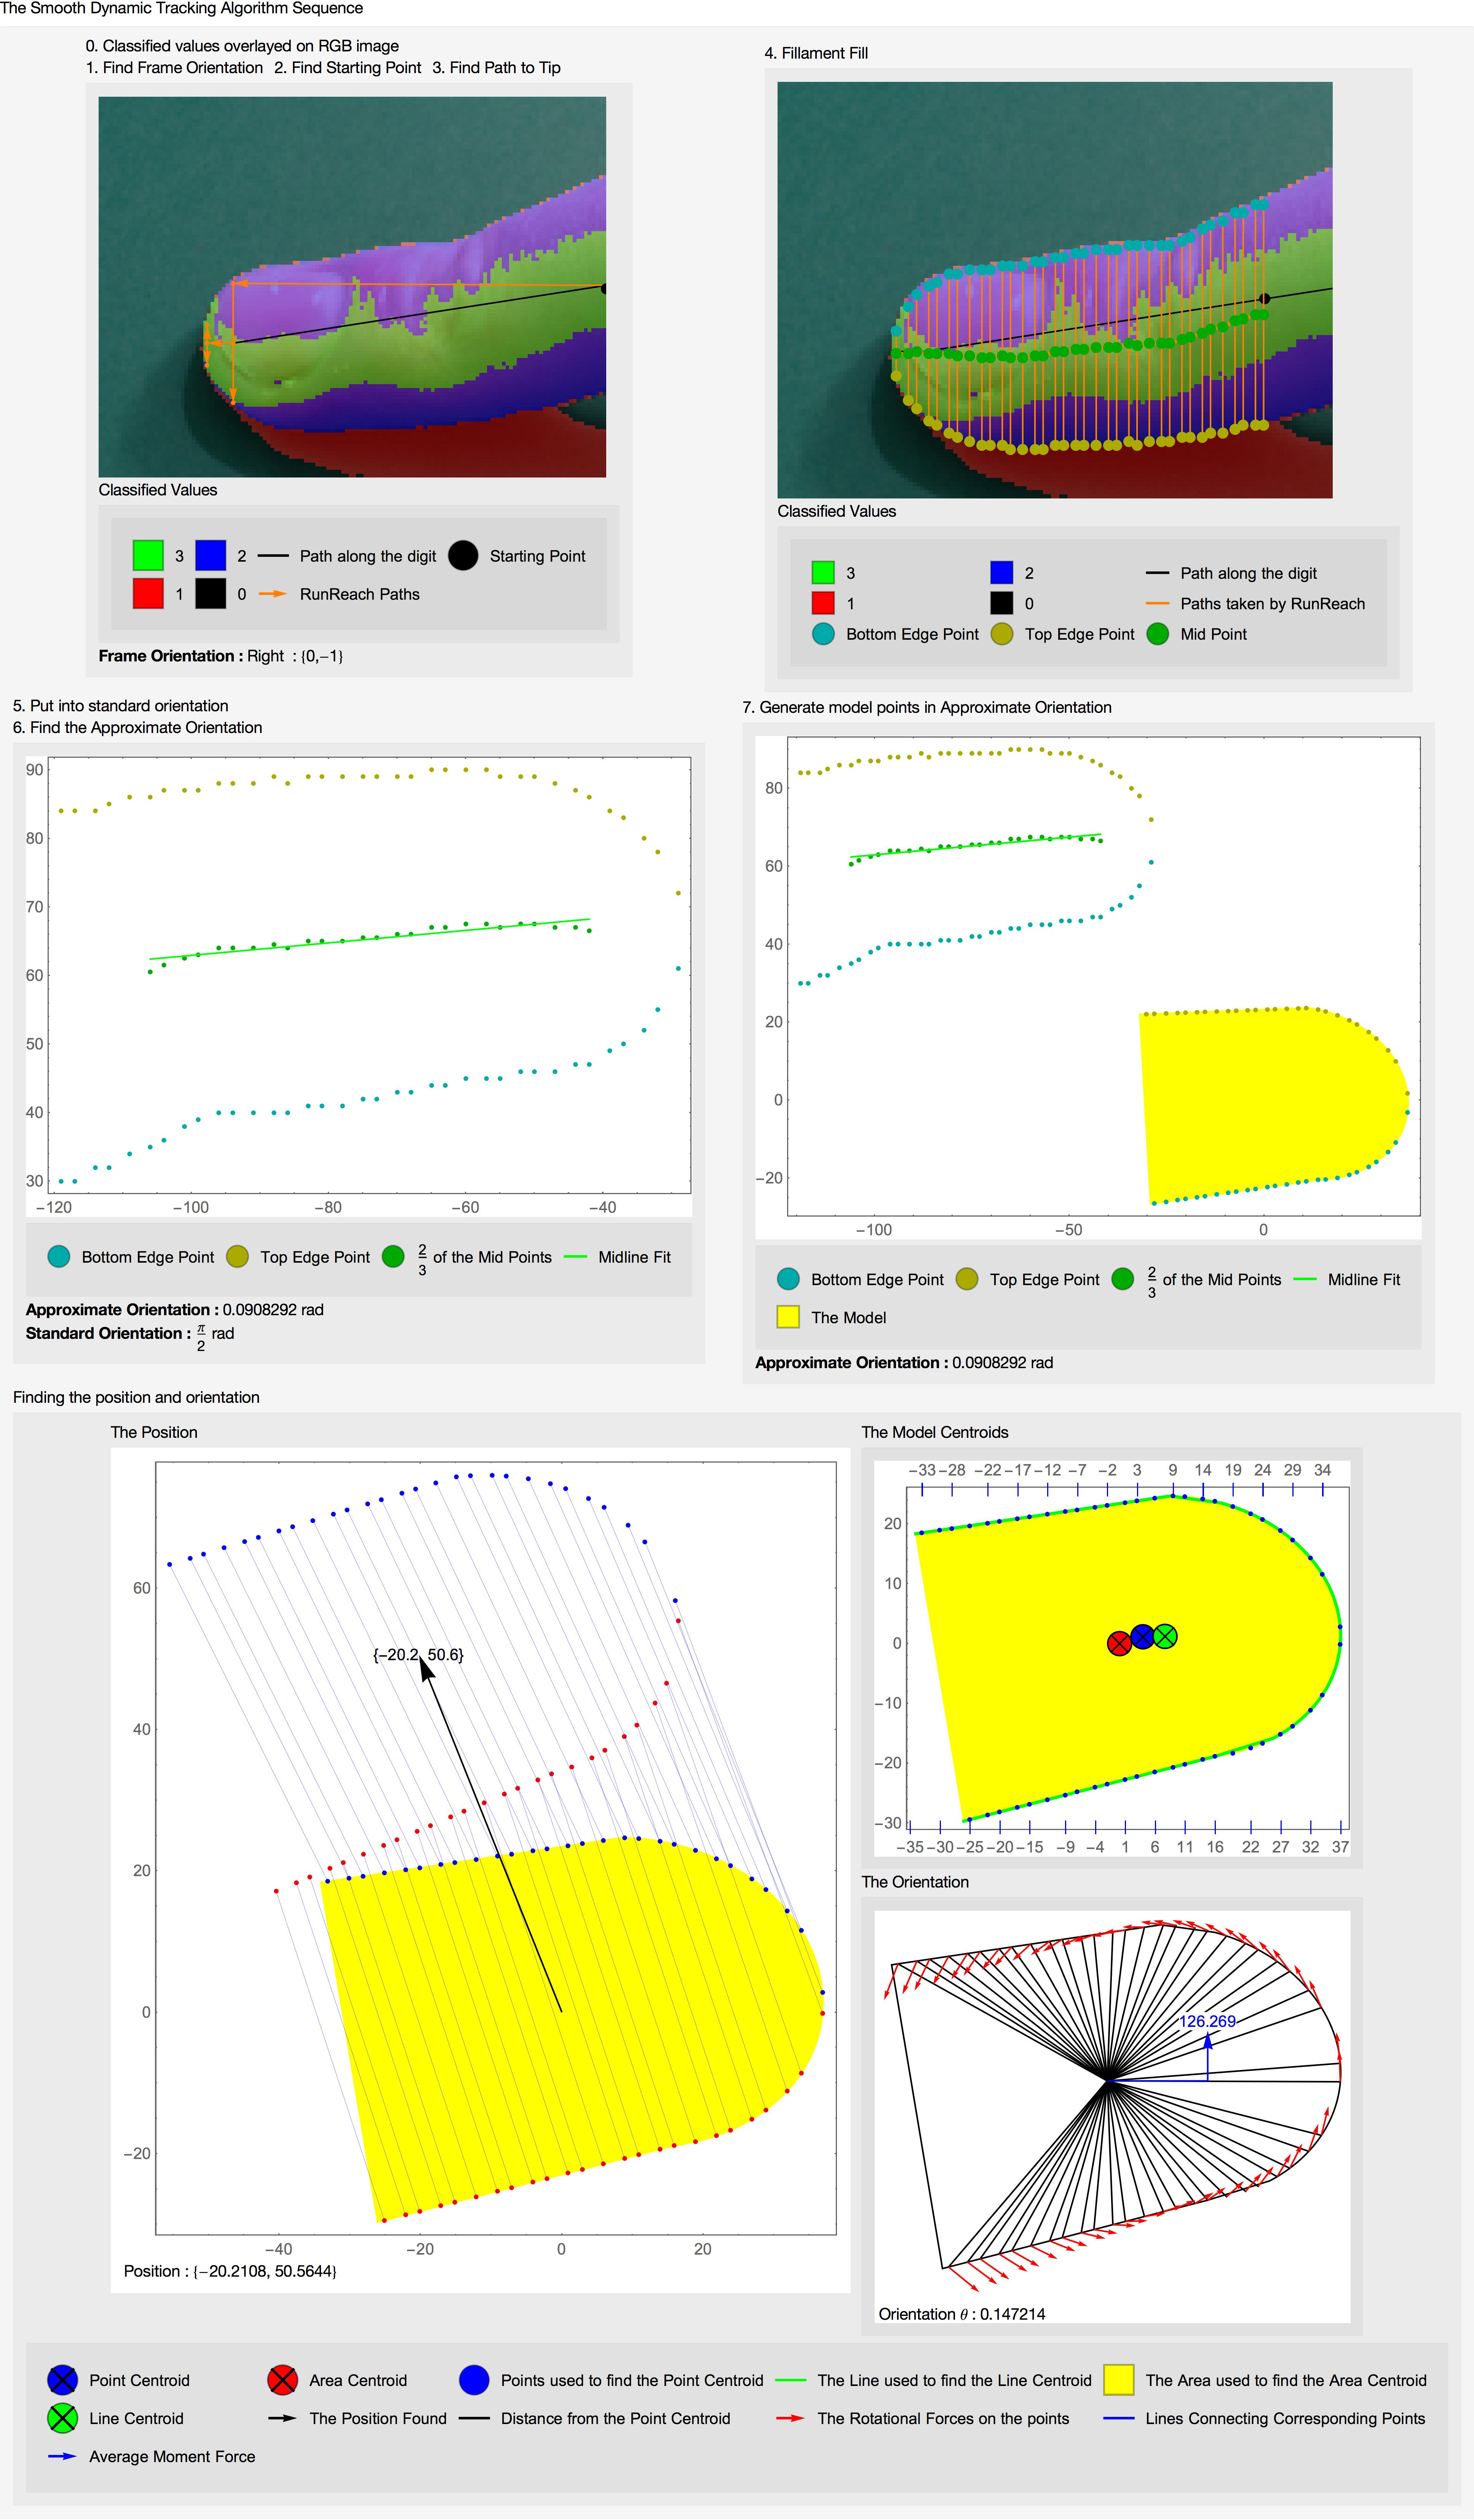
\includegraphics[width=0.85\textwidth]{Chapter4/Figs/Smooth_Dynamic_Sequence.jpg}
    \caption{Smooth Dynamic Sequence}\label{fig:SmoothDynamicSequence}
\end{figure}

In practice, the area centroid is not perfect, but generally locates the digit with an accuracy of two or three pixels, and the orientation within a degree. This accuracy is sufficient for the smooth motion detection algorithm, which operates upon the small scale image. When the movement of the digit falls below the ICWsS threshold, an easy refinement to this shape-fitting algorithm is made by finding the point centroid for the current model orientation, and adjusting the position and orientation accordingly. The additional computational effort to gain this refinement is small, but not necessary when tracking the moving digit for our application.
\clearpage
\subsection{ICWaS Method}\label{sec:ICWaS}
The ICWaS method performs three main tasks: cropping the midscale image around the tip; putting the mask into the cropped midscale image coordinates, rendering the model shape as a binary image; and providing a method which aligns successive frames and finding the pixel color differences in the skin color space, thereby showing the blood flow.

\subsubsection{ICWaS Setup}\label{sec:ICWaSSetup}
From the Smooth Movement Tracking (section \ref{sec:SmoothMotionTracking}), we have a model position and orientation in the small scale space. We wish to track the blood flow using the medium scale image, so first we must put the model in the medium scale space. This is as simple as multiplying the coordinates by a scaling factor as shown in section \ref{sec:ScaleSpace}.

Now we want to find the extreme top, bottom, left and right edges of the model in order to crop the midscale image appropriately. The model is comprised of a quadrilateral and an ellipse. To find the extreme edges of the quadrilateral, the algorithm just finds the minimum and maximum values of the coordinates of its vertices. The ellipse's extreme edges can be found using

\begin{minipage}{0.7\textwidth}
\begin{align*}
\begin{array}{ll}
e_1= \Bigg( x_0+\frac{(a-b) (a+b) }{A} \sin \left( \theta \right) & , y_0+A \cos \left( \theta \right) \Bigg)\\
e_2=  \Bigg( x_0-\frac{(a-b) (a+b)}{A} \sin \left( \theta \right) & , y_0-A \cos \left( \theta \right) \Bigg)\\
e_3=  \Bigg( x_0-B \cos \left( \theta \right)  & , y_0-\frac{(a-b) (a+b) }{B} \sin \left( \theta \right) \Bigg)\\
e_4=  \Bigg( x_0+B \cos \left( \theta \right)  & , y_0+\frac{(a-b) (a+b) }{B} \sin \left( \theta \right) \Bigg)\\
\end{array} \\
 \text{where}\quad 
\begin{array}{c}
A=\sqrt{a^2 \tan ^2(\theta )+b^2} \\
B=\sqrt{a^2+b^2 \tan ^2(\theta )} \\
-\frac{\Pi}{2}< \theta < \frac{\Pi}{2}
\end{array}
\end{align*}
\end{minipage}%%%%%%%%%%%%%%%%
\begin{minipage}{0.3\textwidth}
 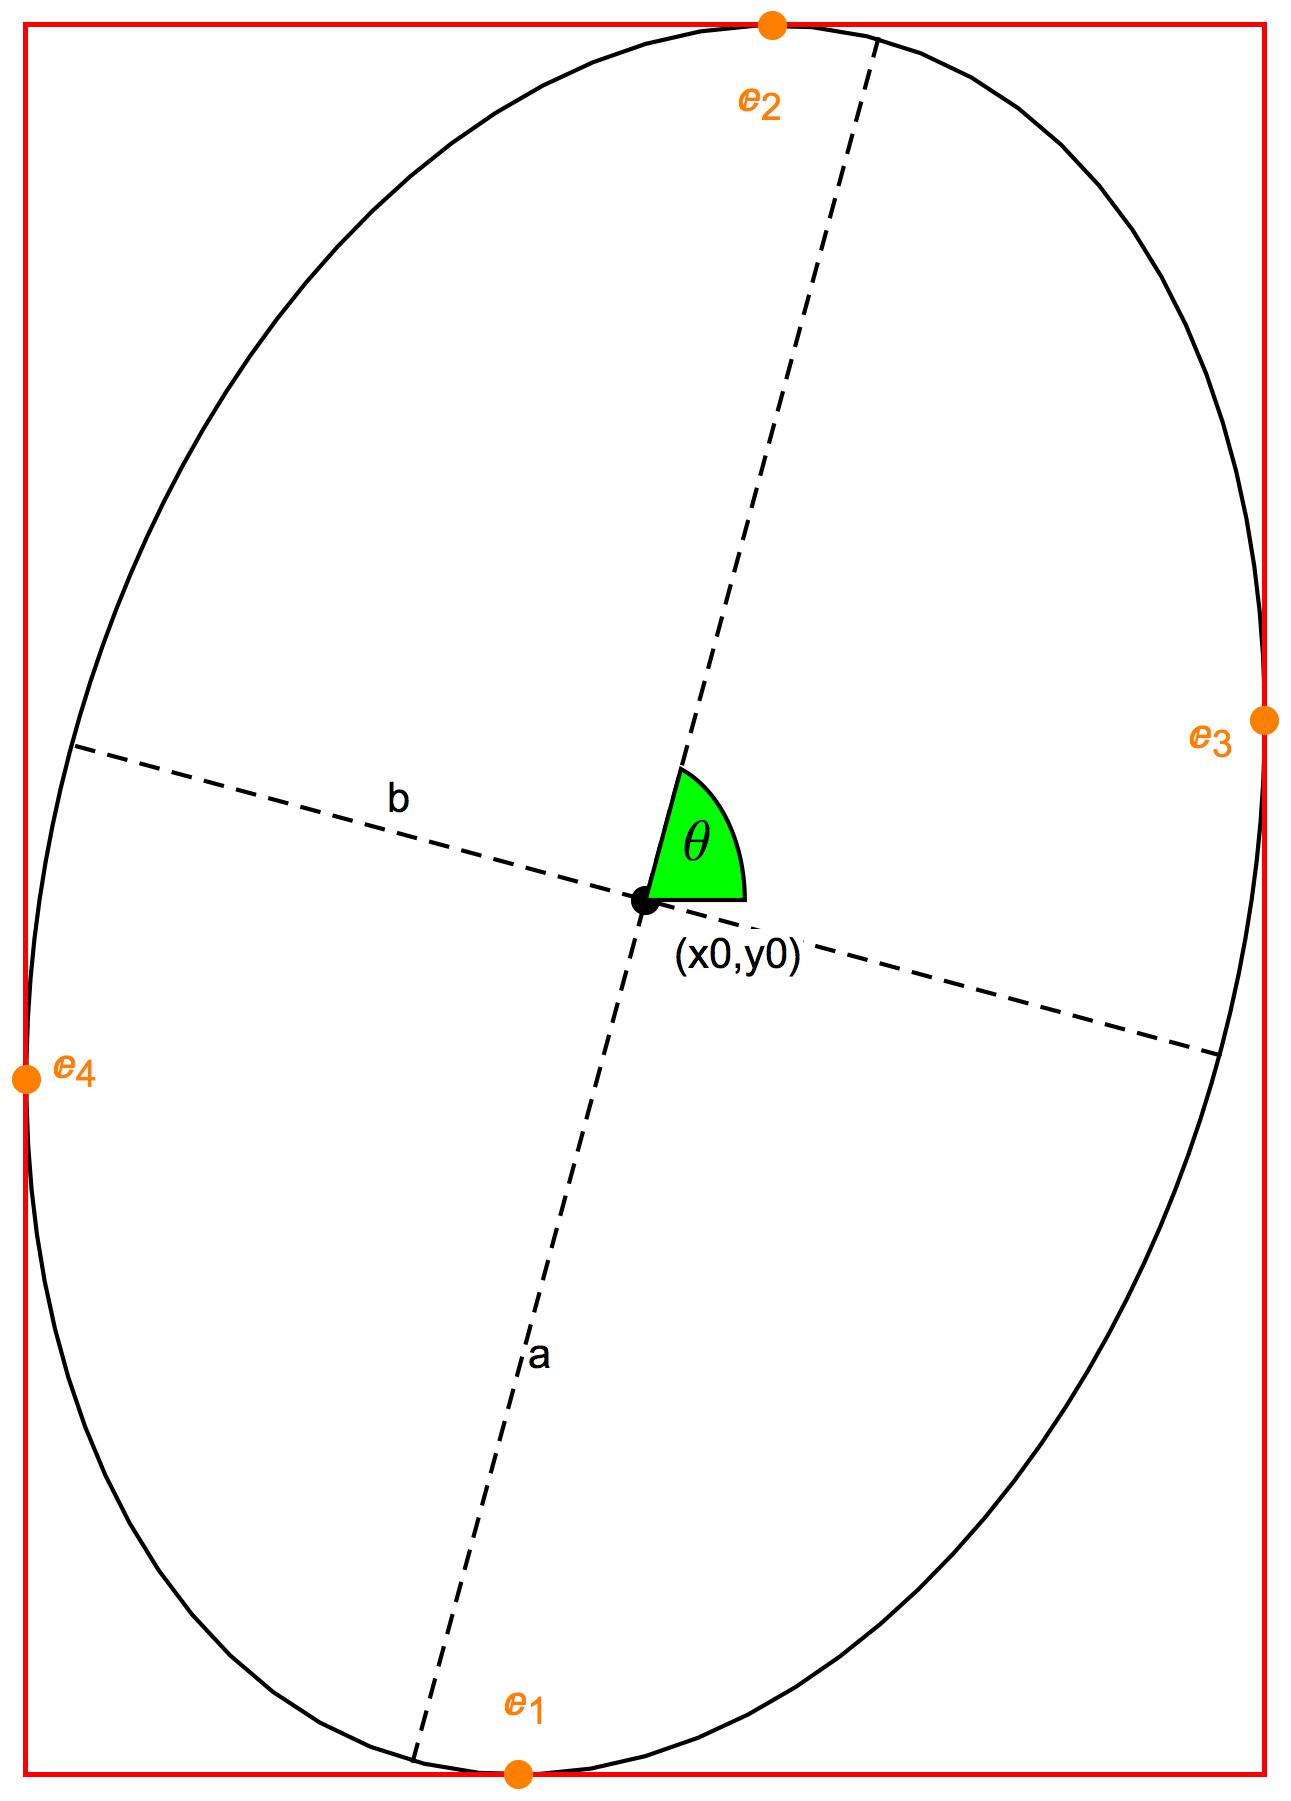
\includegraphics[width=\textwidth]{Chapter4/Figs/Elliptical_Bounds.jpg}
\end{minipage}


However, we only want to include extreme points which lie on the curve which models the tip. The curve which models the tip is the part of the ellipse which falls between the two points on the quadrilateral closest to the tip. We can check if the extreme edges of the ellipse are on this part of the curve by checking that they lie at an angular position between the angles at which the tipmost quadrilateral points lie.

Now we have the extreme edges of the model. These points are used to find a bounding box, which includes all the tip pixels in the small scale space. Translating these to the medium scale space, we subtract the scaling factor from the lower coordinates and add the scaling factor to the higher coordinates, ensuring that the box does not crop any pixels from the digit in the medium scale space. We now take the medium scale RGB image, crop it to the model bounding box, and pass the extracted tip image to the skin color space processing routines. The grayscale image is saved as a template for the template matching algorithm.

During a finger press, we expect the flesh to deform around the tip, making the edges of the digit unreliable for alignment. So we wish to construct a binary mask which tells the template matching algorithm which pixels to use for alignment. Using OpenCV's drawing routines, we render the model in the midscale tip image coordinates. This is done in a way which actually renders the model 'slightly' by four or five pixels smaller than the model proper. This effectively eliminates the edge of the digit next to the background, pushing the algorithm to rely on features which do not deform, such as the nail.

\subsubsection{Blood Flow}\label{sec:BloodFlow}

\begin{figure}[h!]
  \centering
    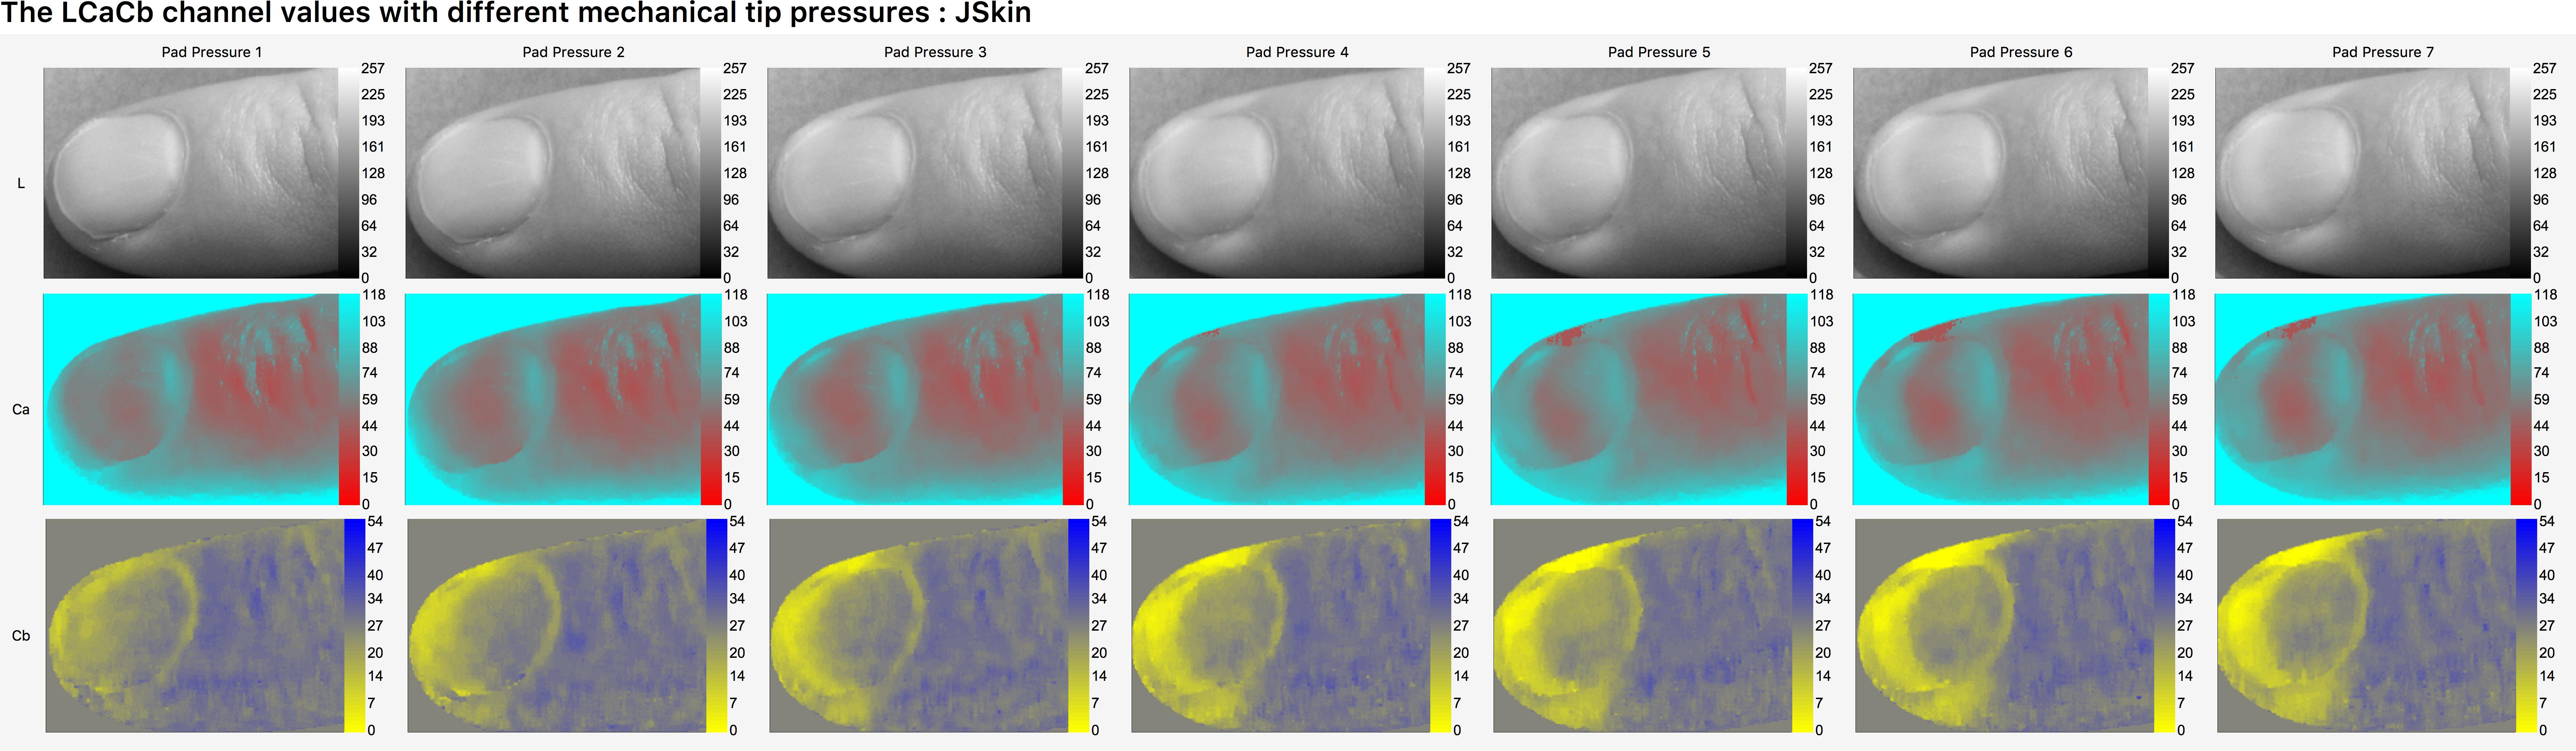
\includegraphics[width=1.00\textwidth]{Chapter4/Figs/Final_Fig_Channels_JSkin.jpg}
    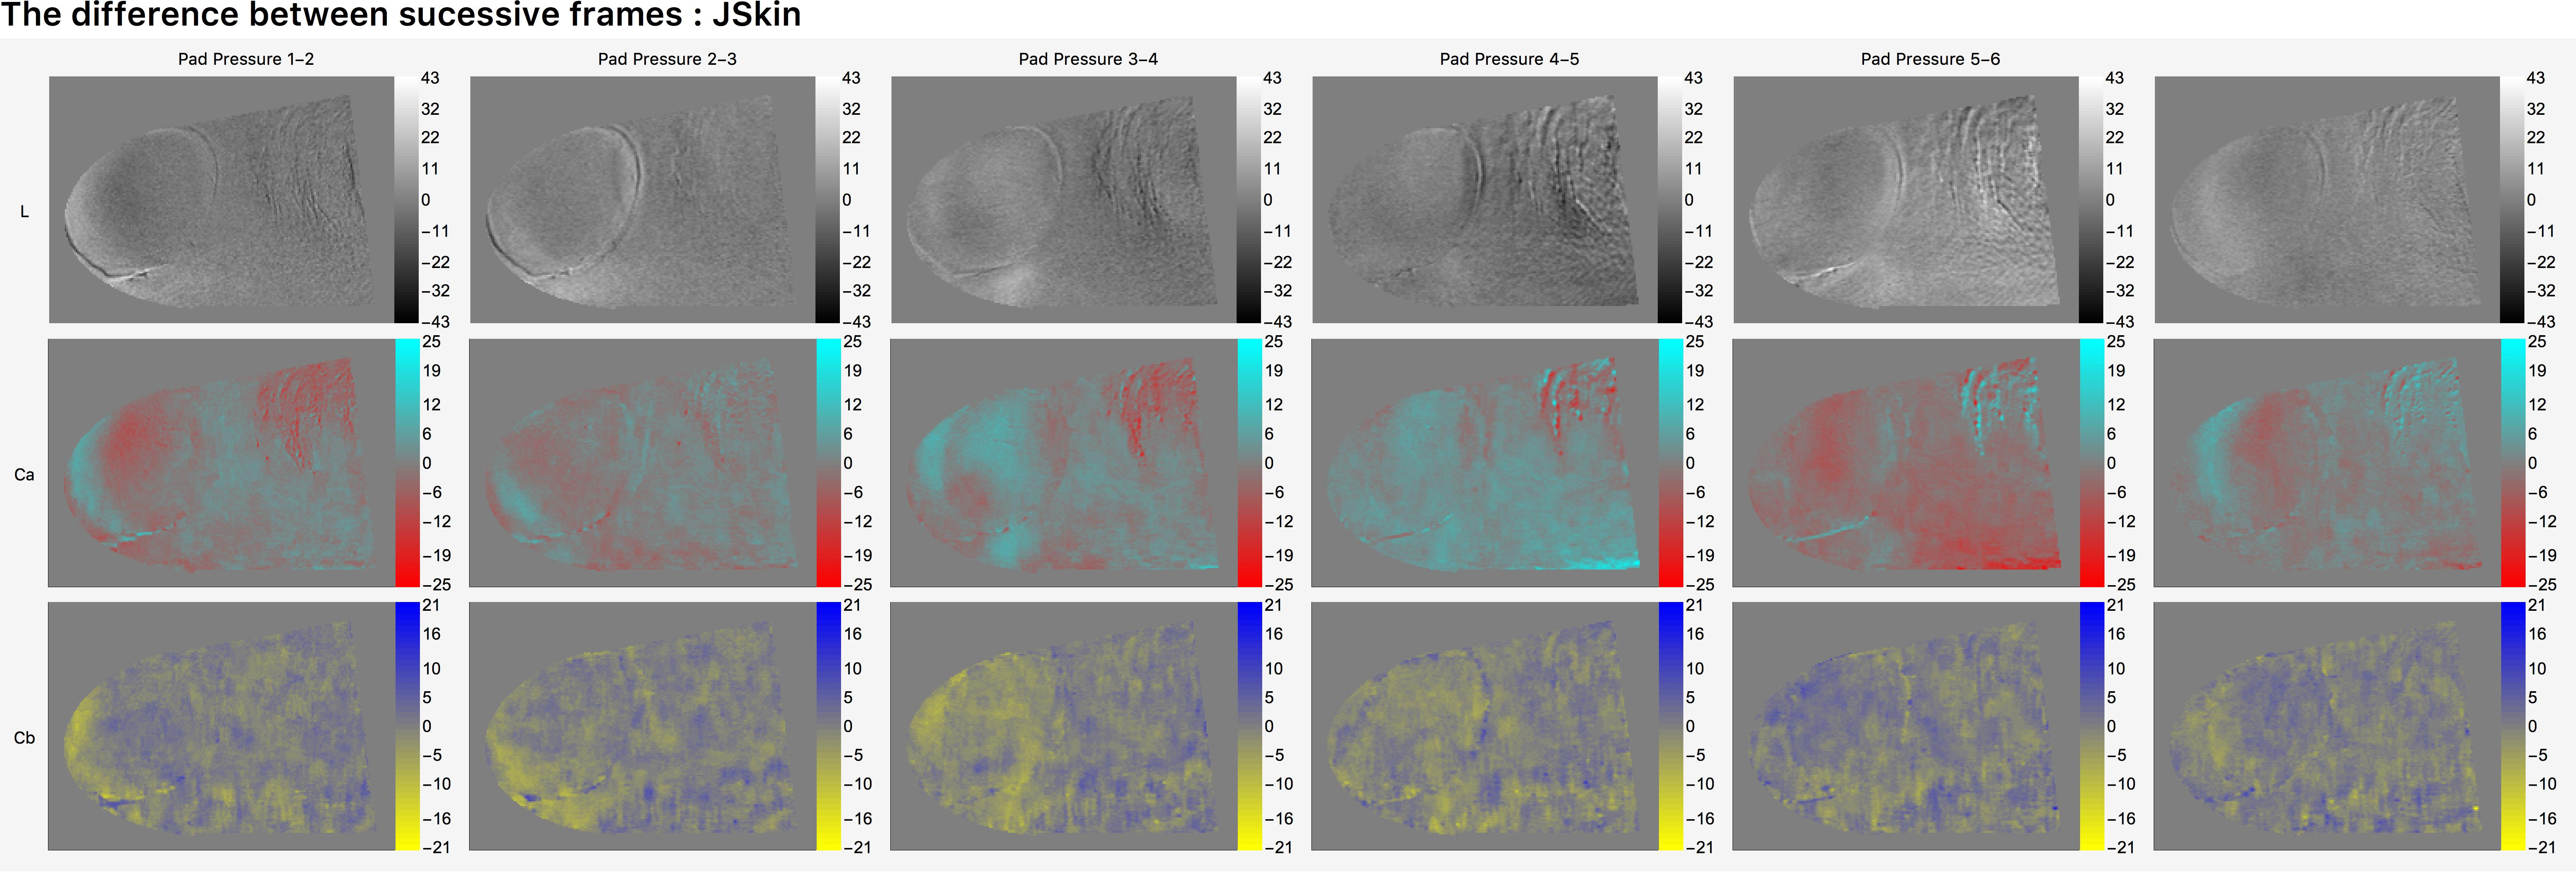
\includegraphics[width=0.86\textwidth]{Chapter4/Figs/Final_Fig_Difference_JSkin.jpg}
    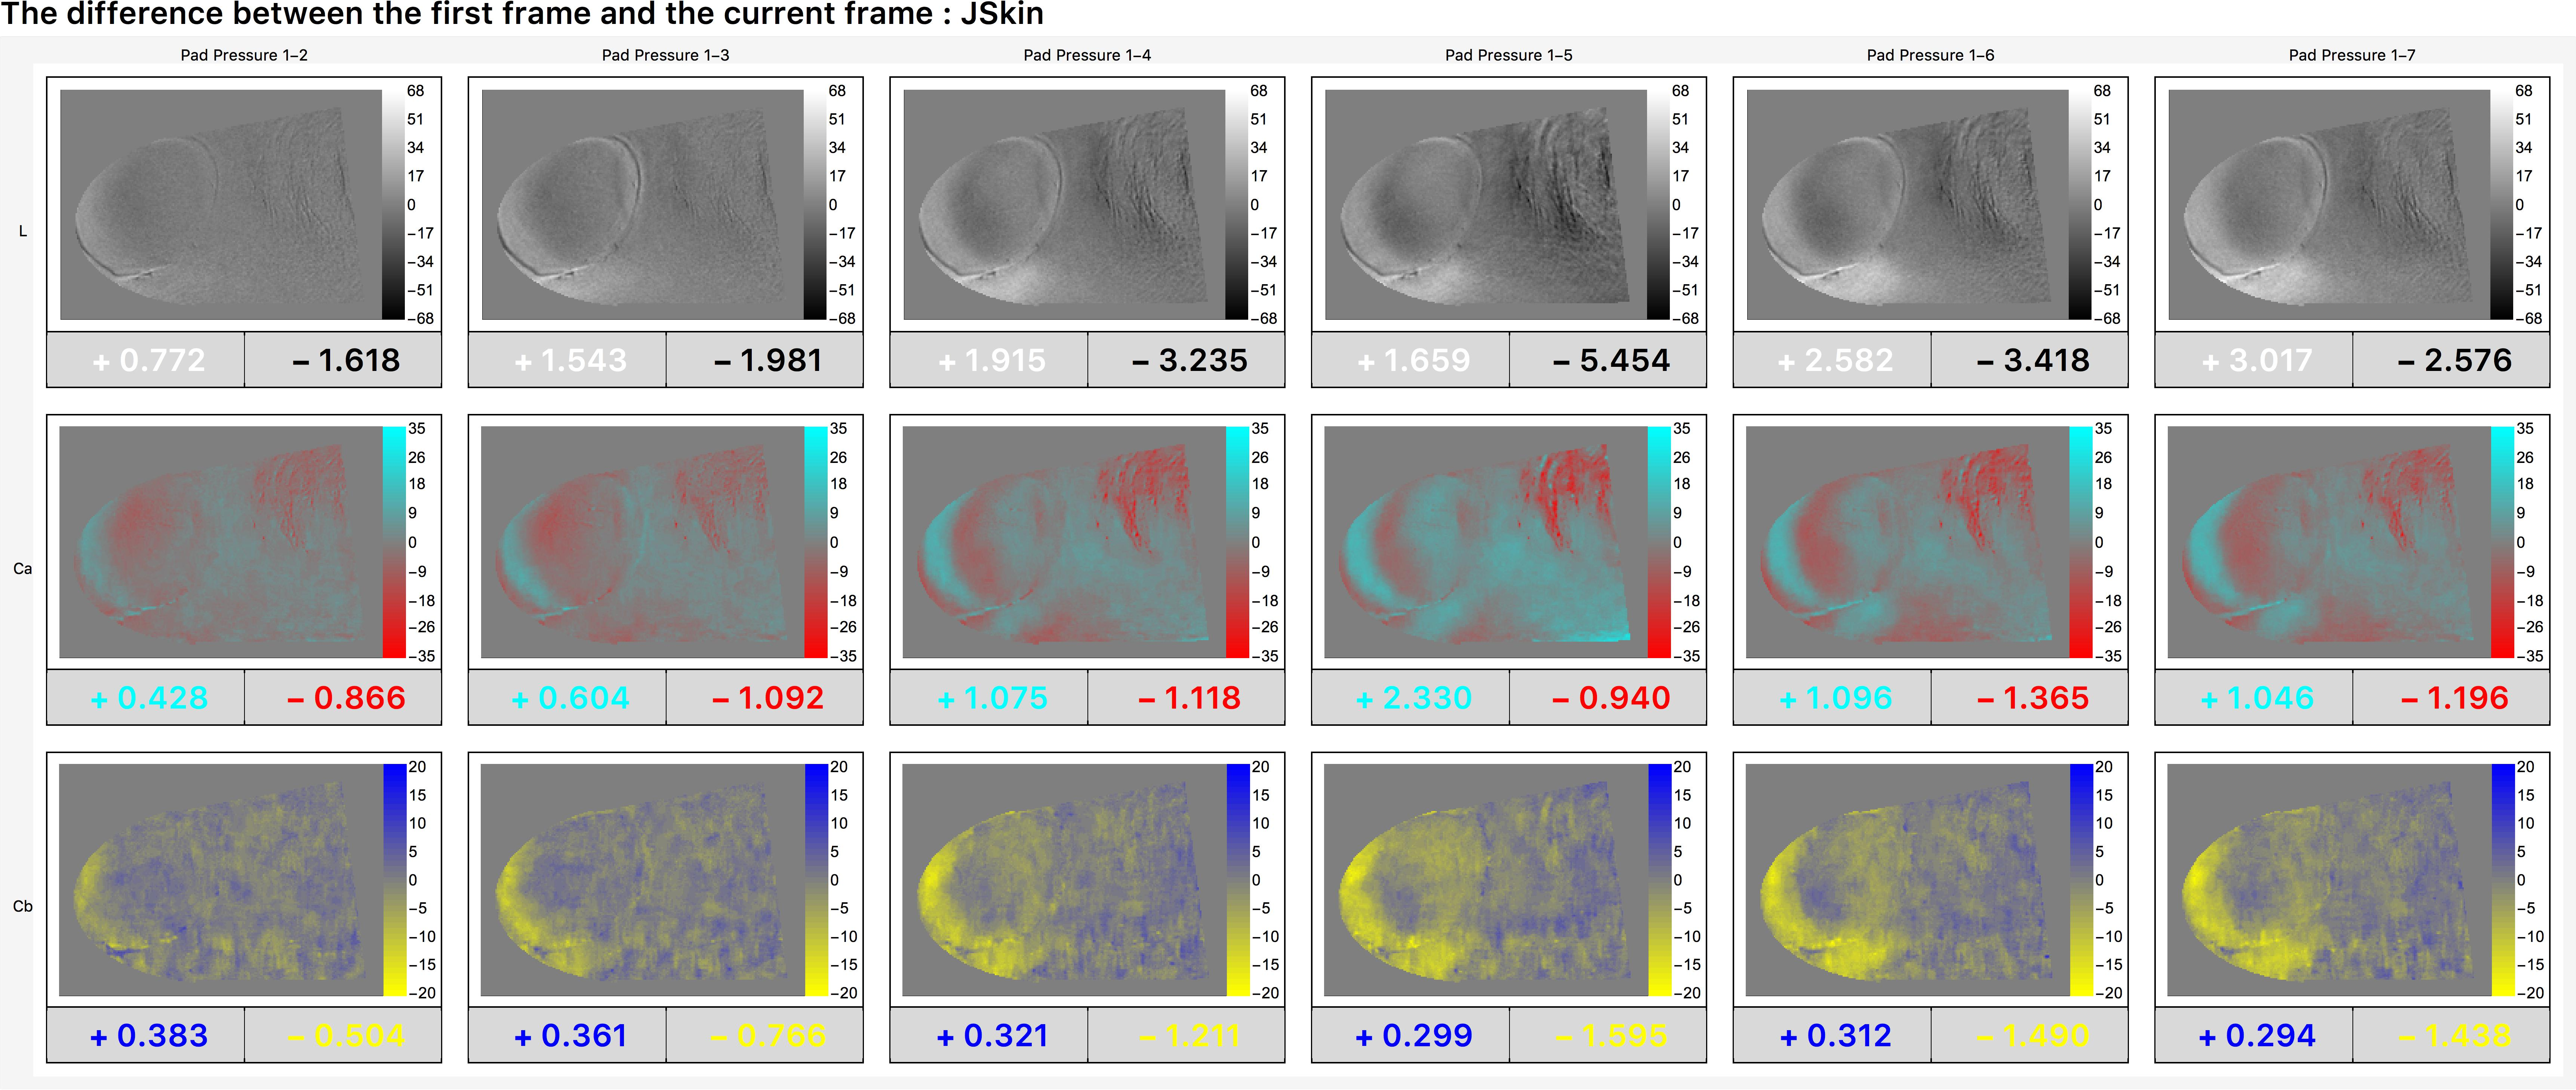
\includegraphics[width=0.86\textwidth]{Chapter4/Figs/Final_Fig_Total_Difference_JSkin.jpg}
    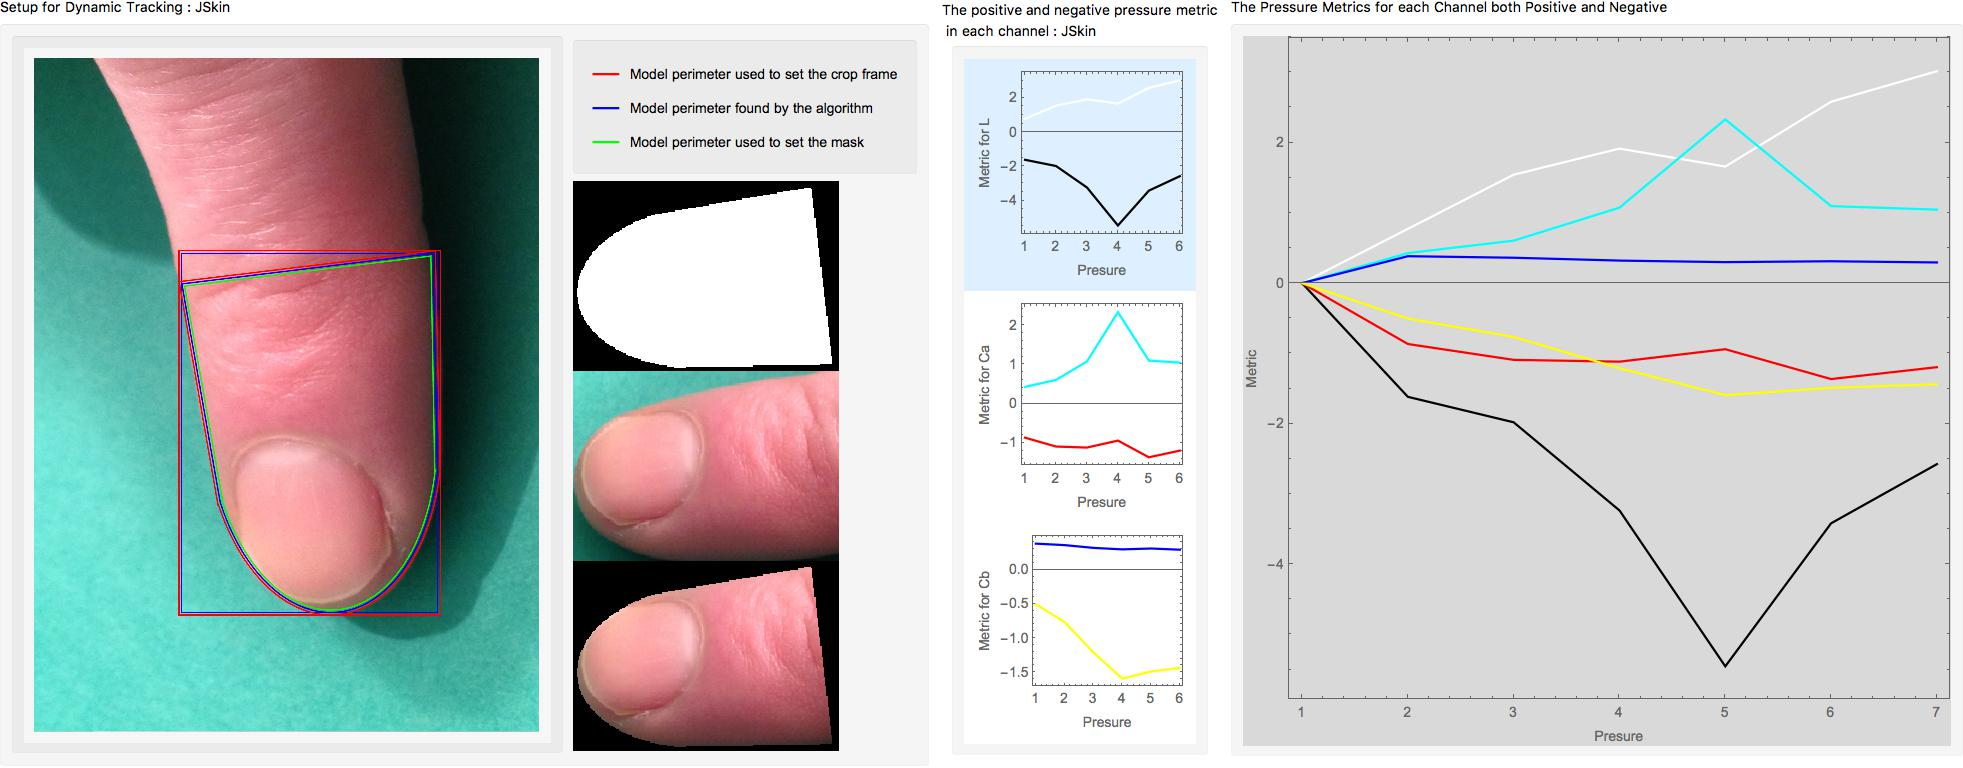
\includegraphics[width=1.00\textwidth]{Chapter4/Figs/Final_Fig_Misc_JSkin.jpg}
    \caption{The resulting sequence of images from the ICWaS algorithm followed by the differences. The metric is the result of summing the positive and negative changes separately and dividing by the number of pixels. Finally the initial image of the sequence is shown with the model outline, the slightly larger model used to set the crop frame and the slightly smaller model used for setting the mask.}\label{fig:ICWaSResultJSkin}
\end{figure}

\begin{figure}[h!]
  \centering
    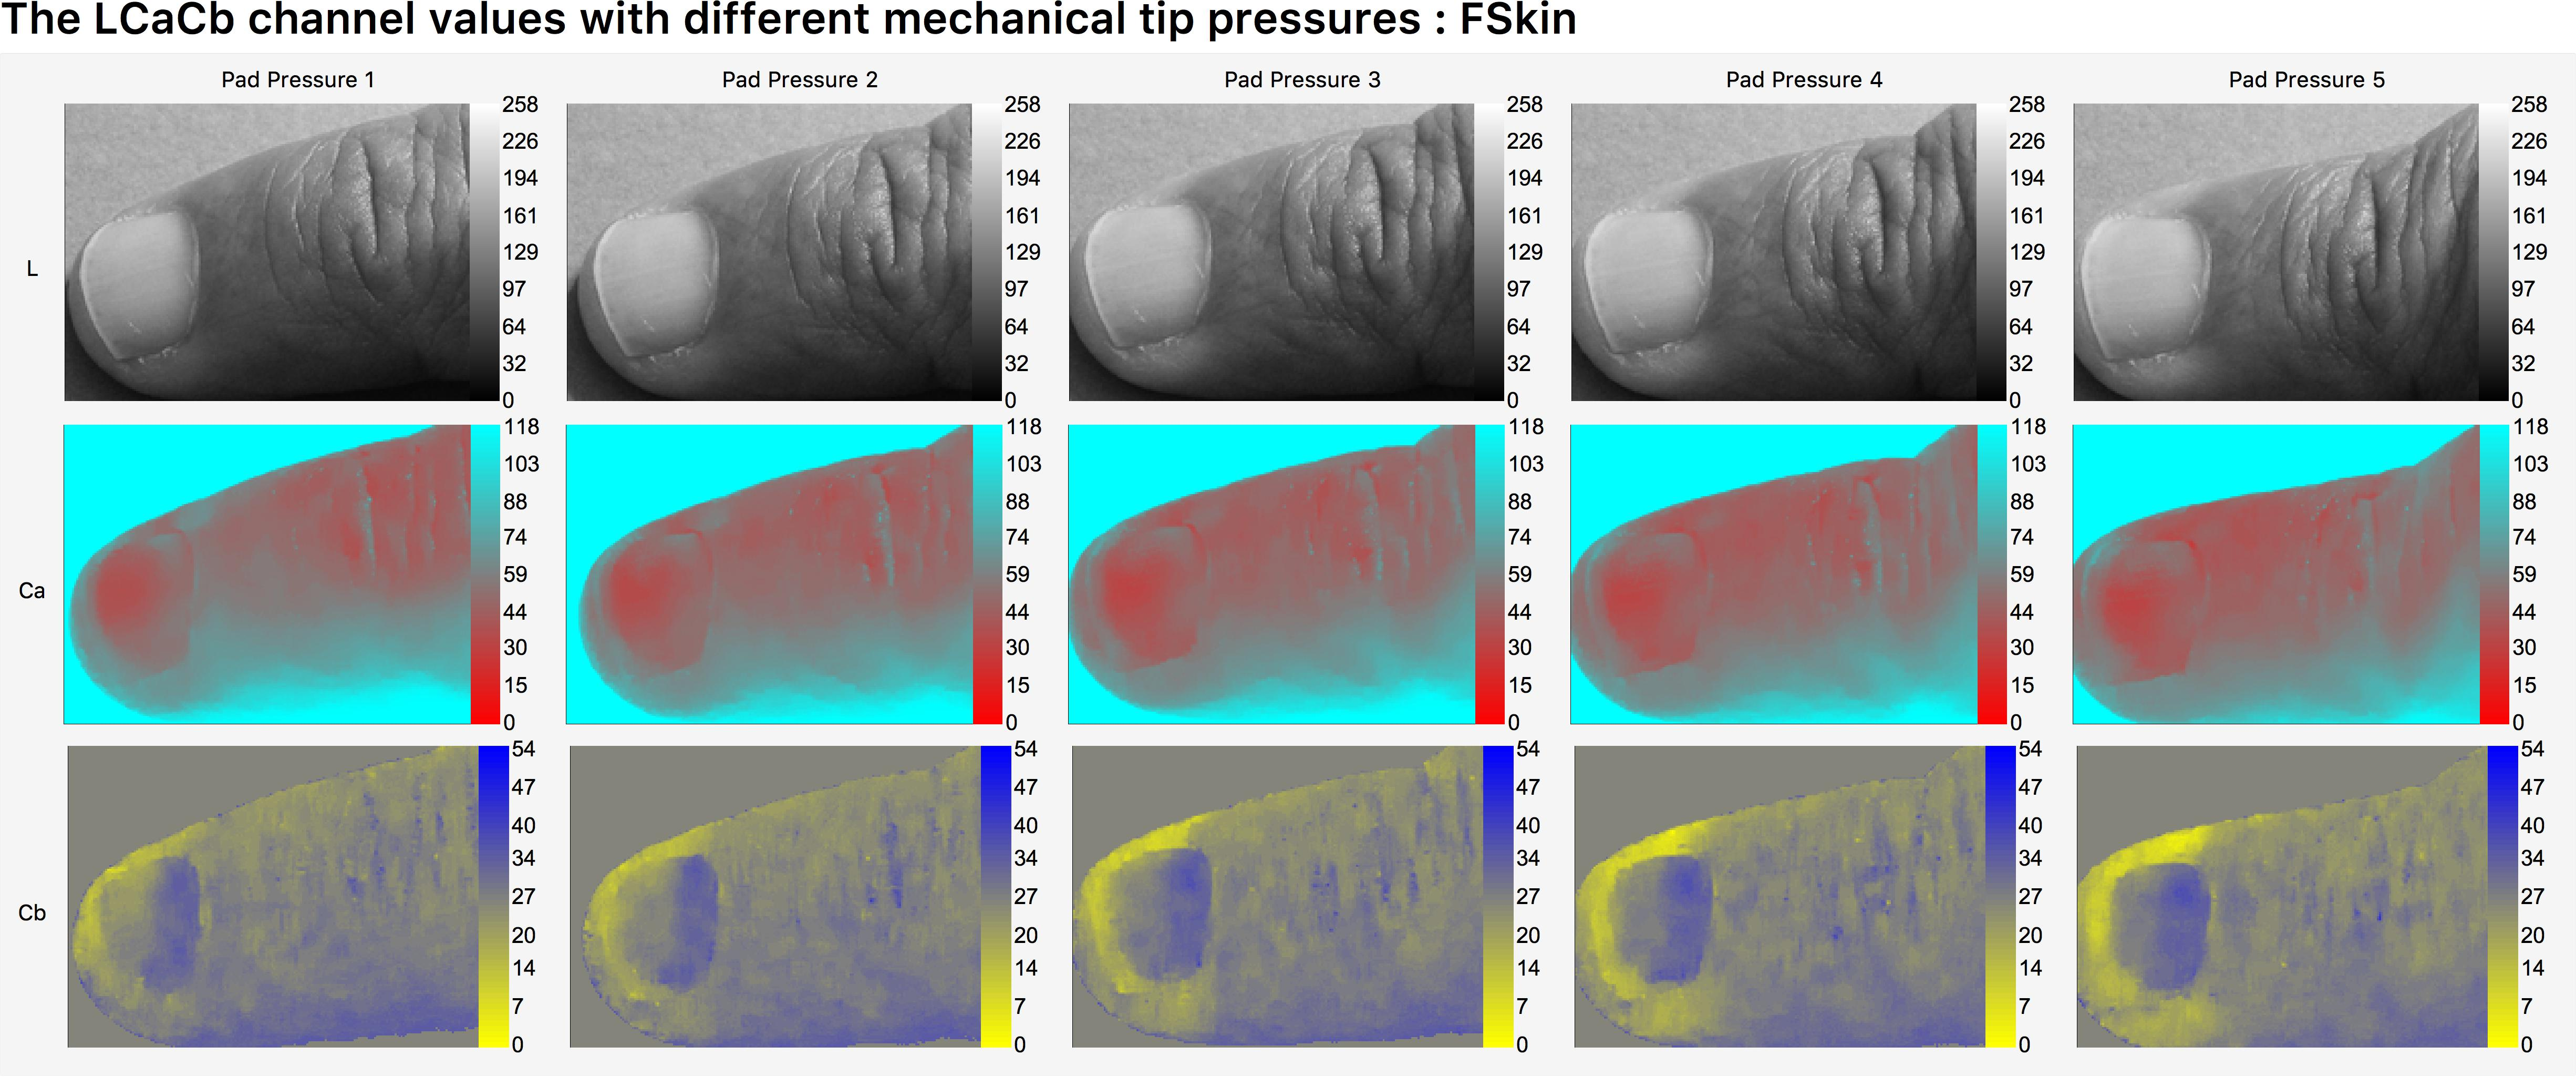
\includegraphics[width=0.820\textwidth]{Chapter4/Figs/Final_Fig_Channels_FSkin.jpg}
    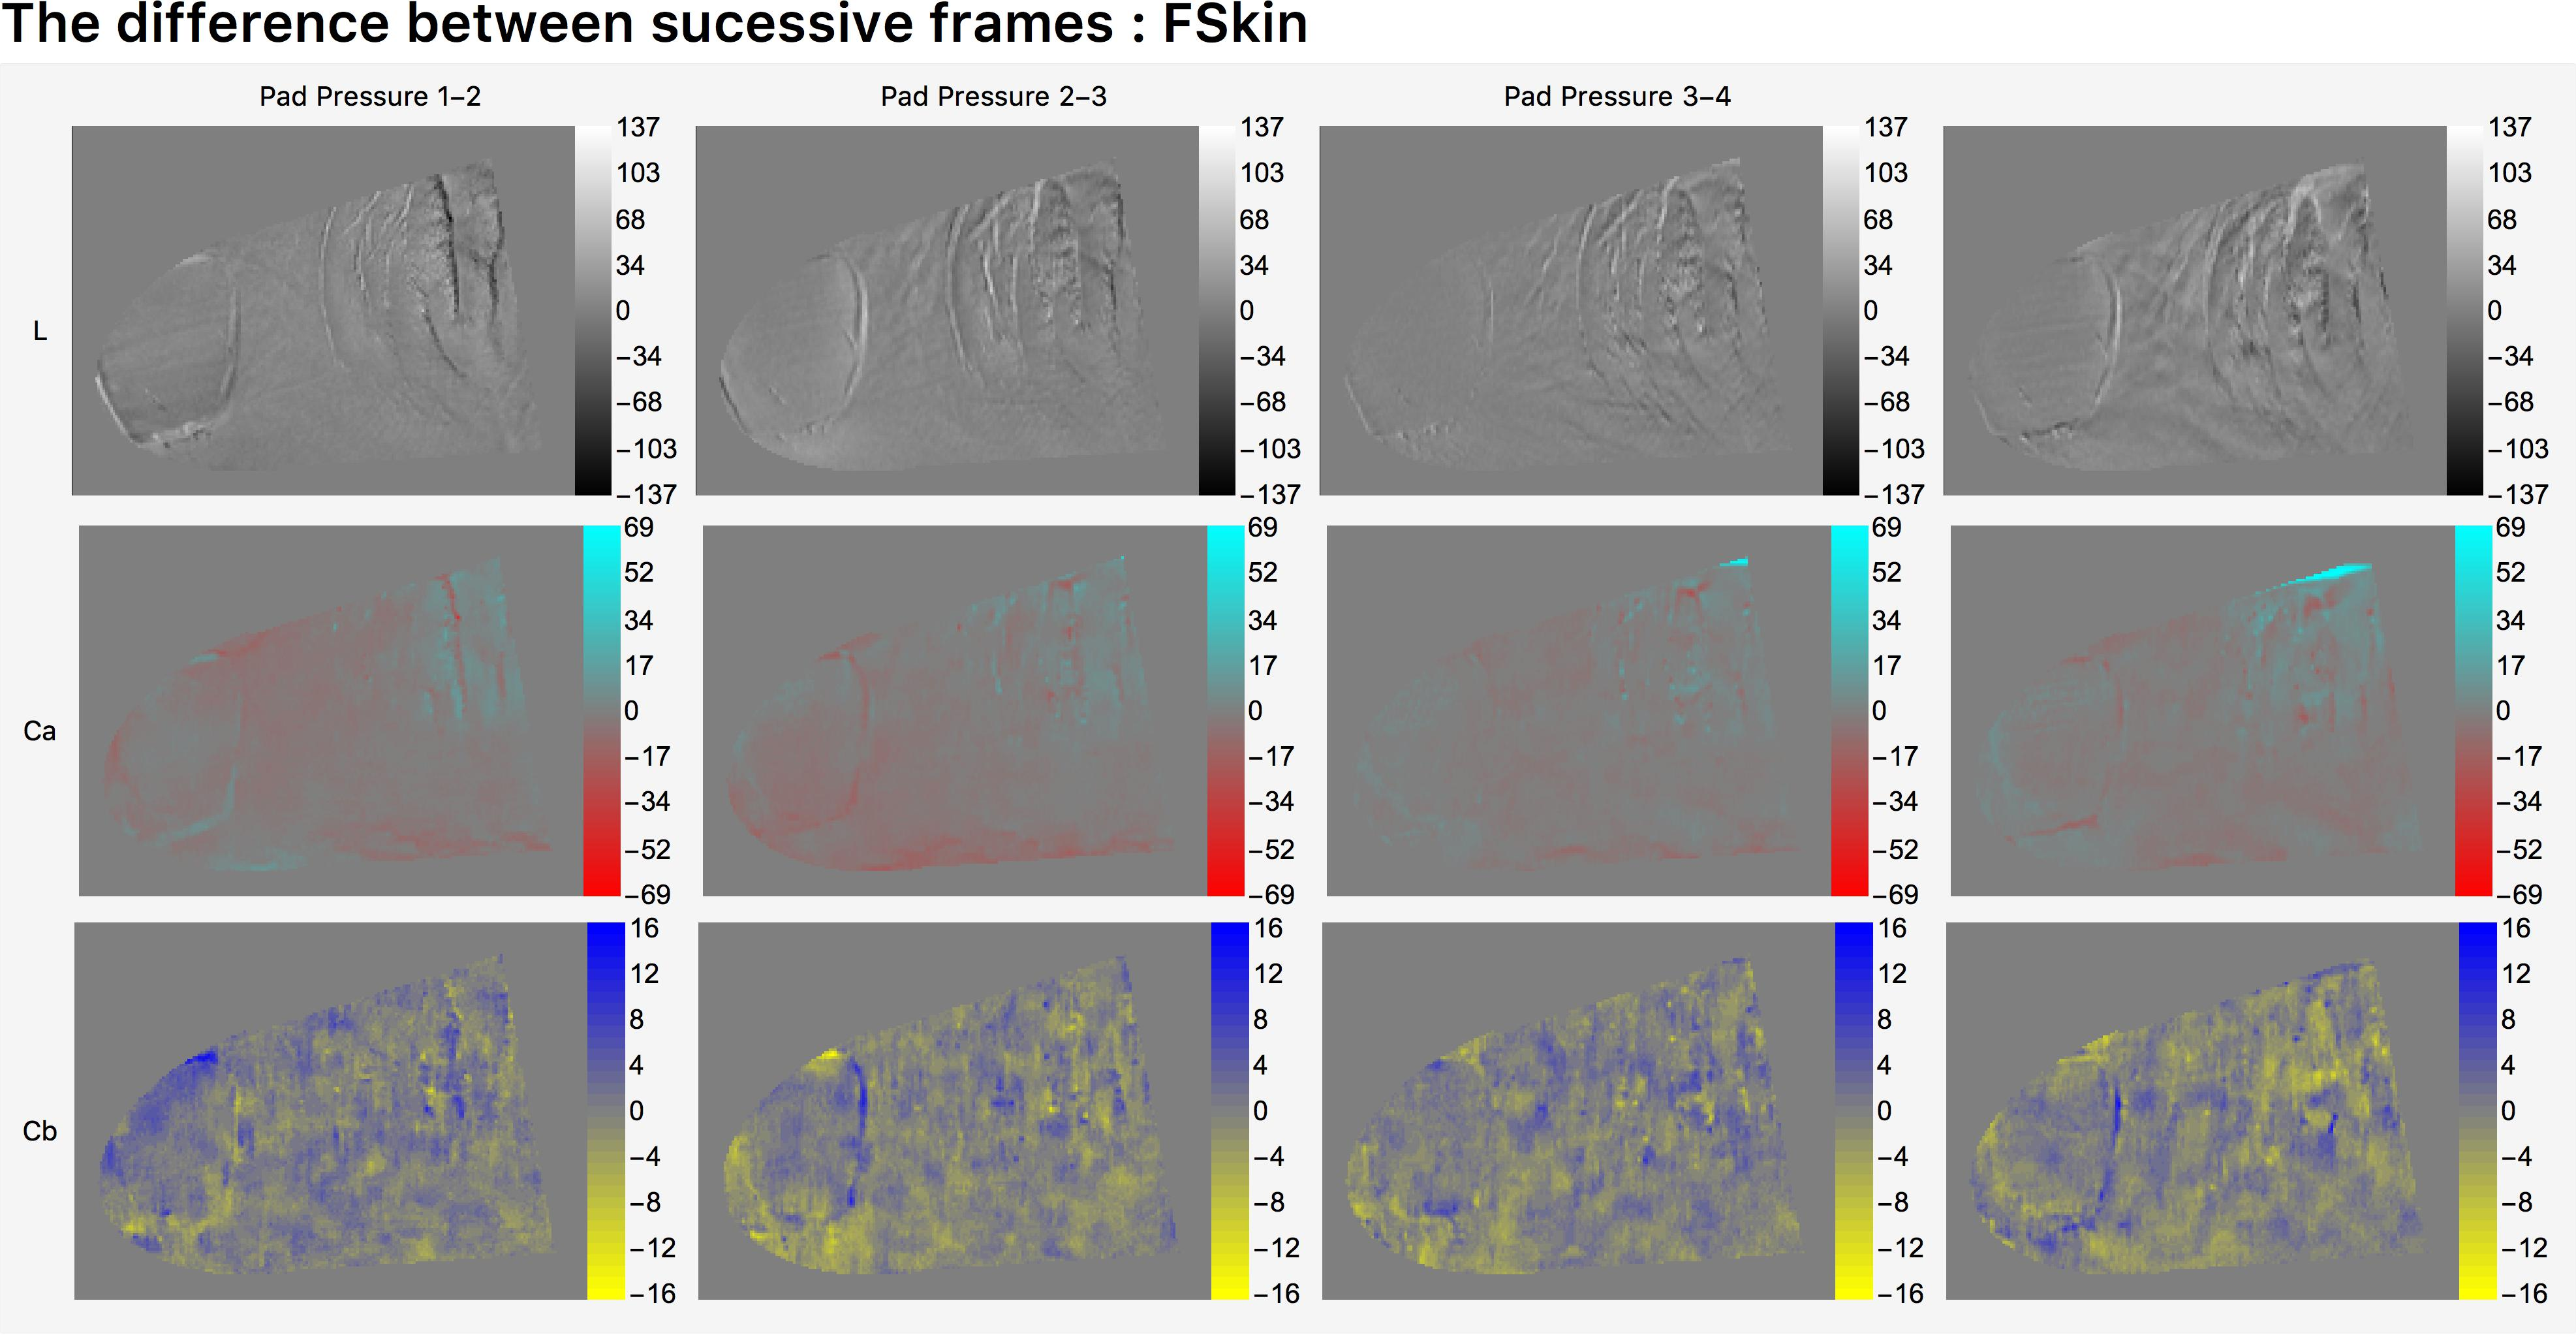
\includegraphics[width=0.660\textwidth]{Chapter4/Figs/Final_Fig_Difference_FSkin.jpg}
    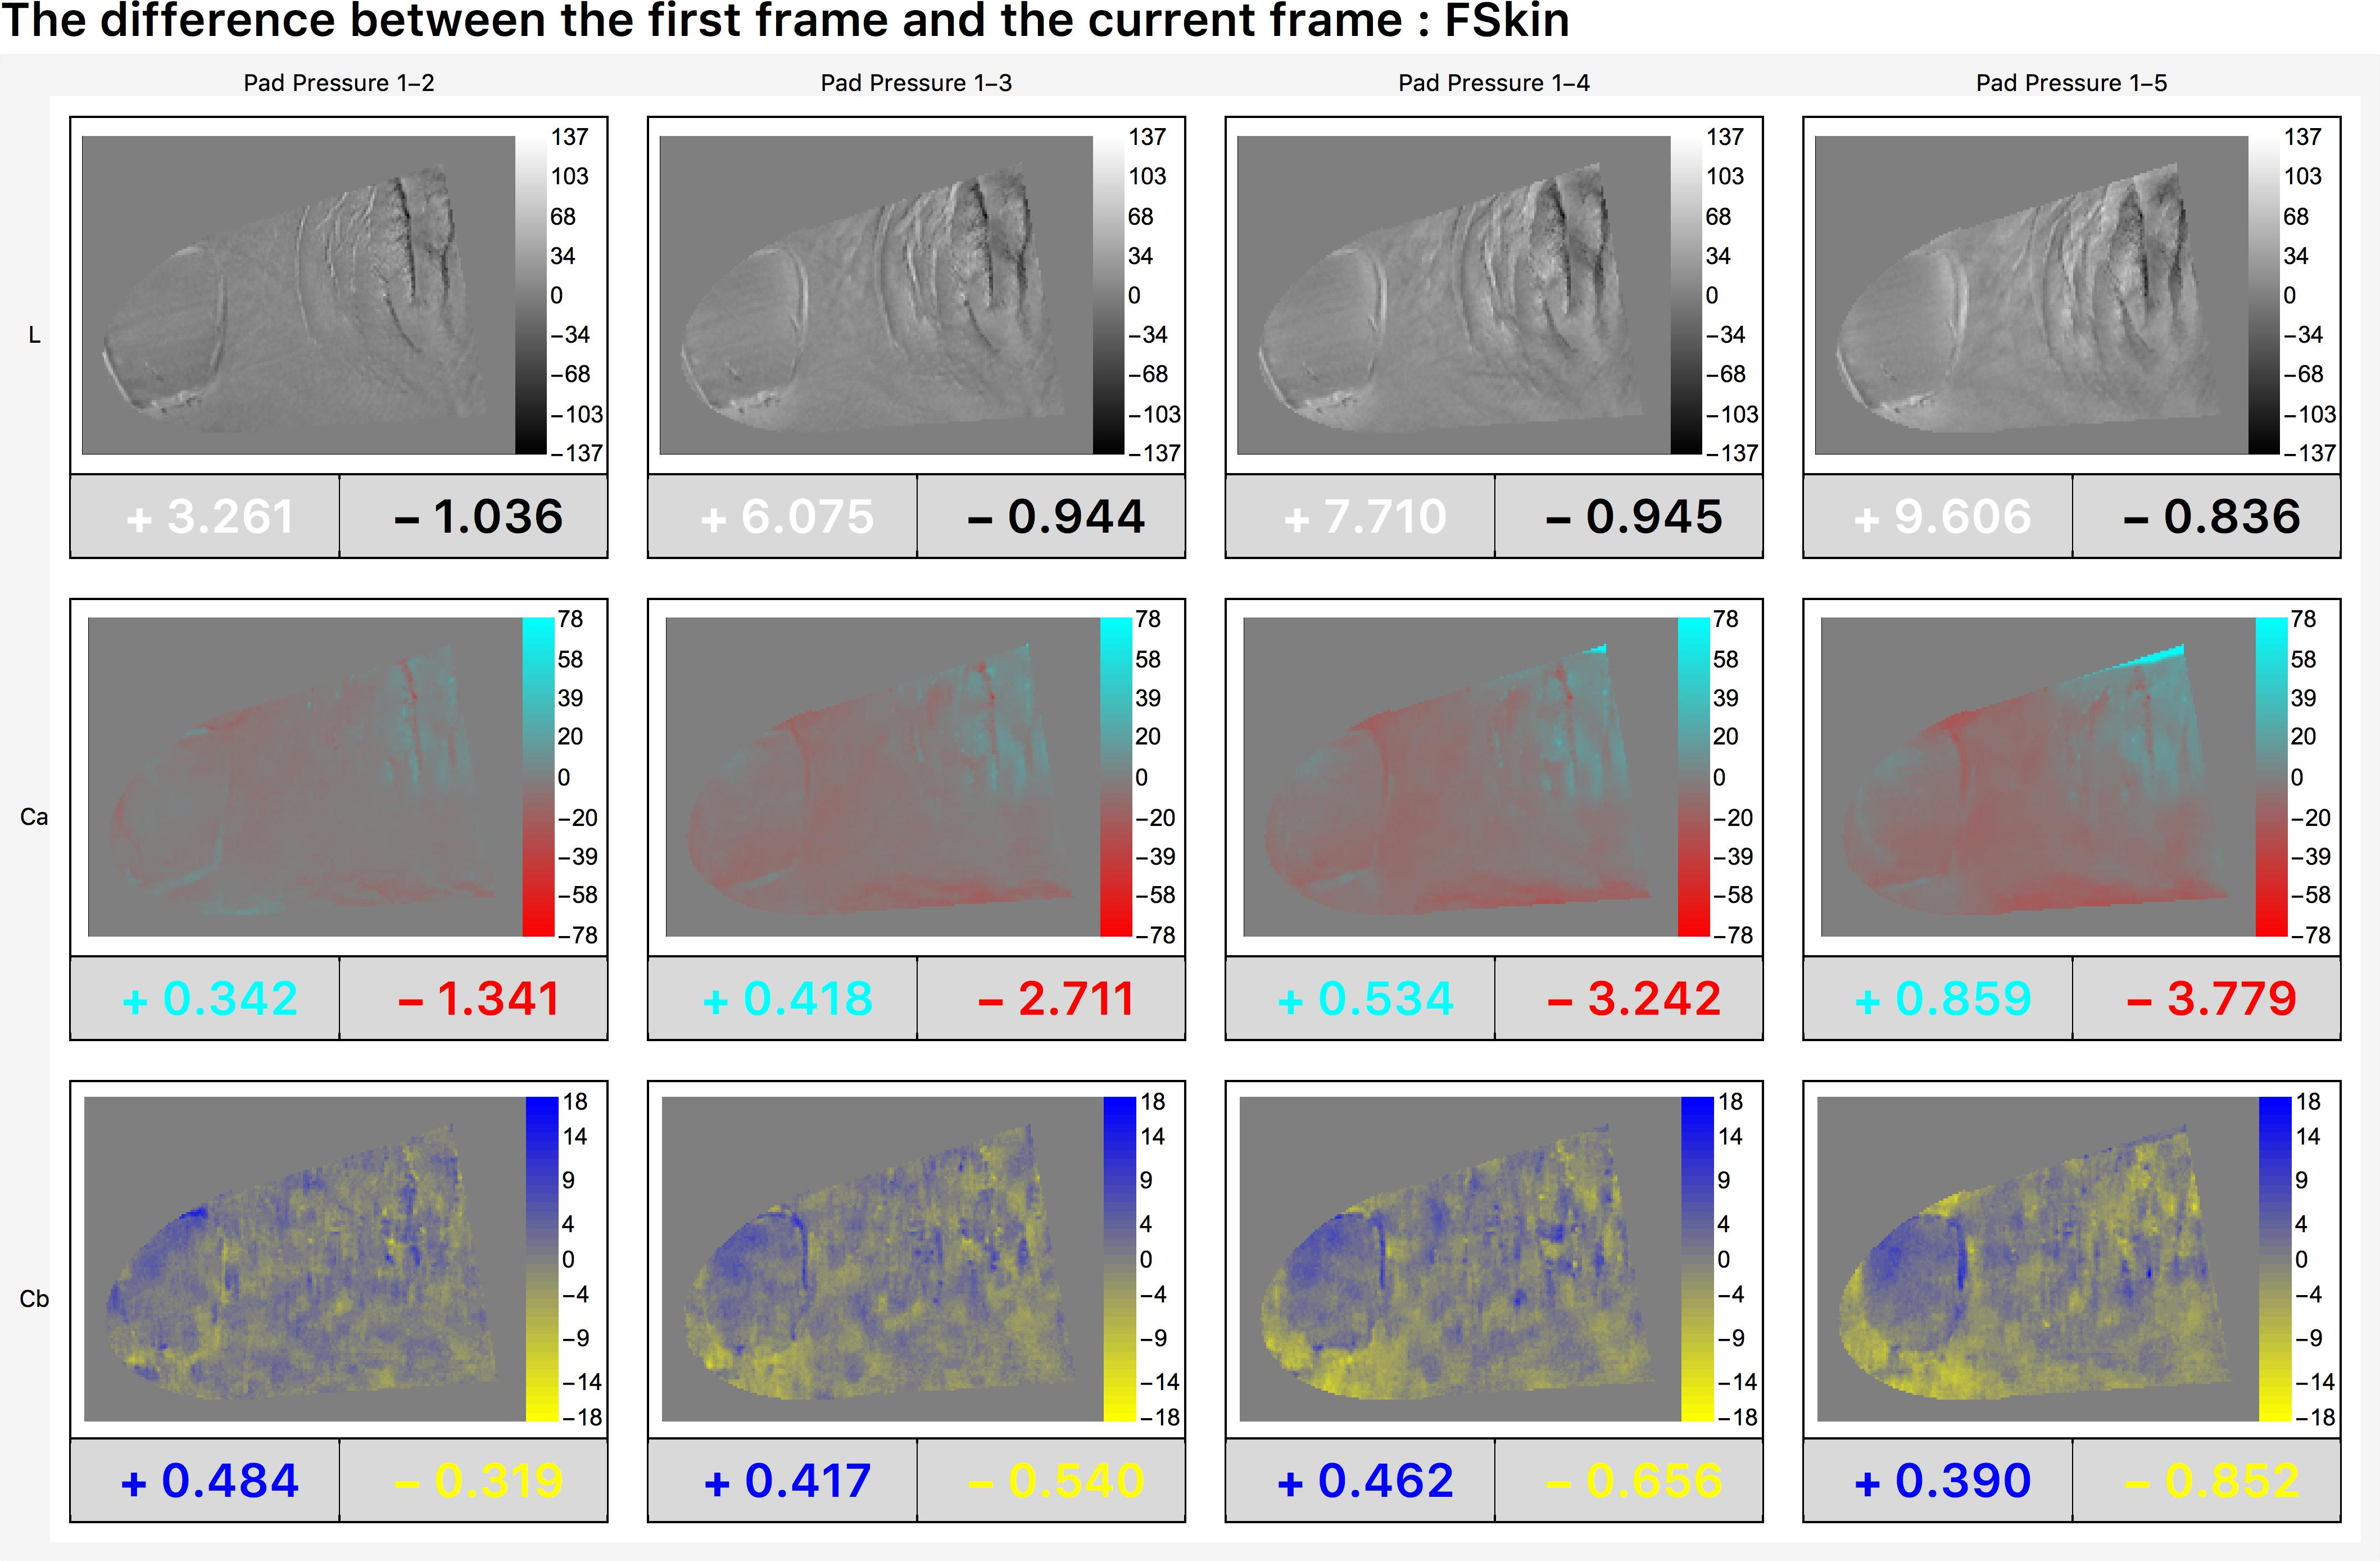
\includegraphics[width=0.660\textwidth]{Chapter4/Figs/Final_Fig_Total_Difference_FSkin.jpg}
    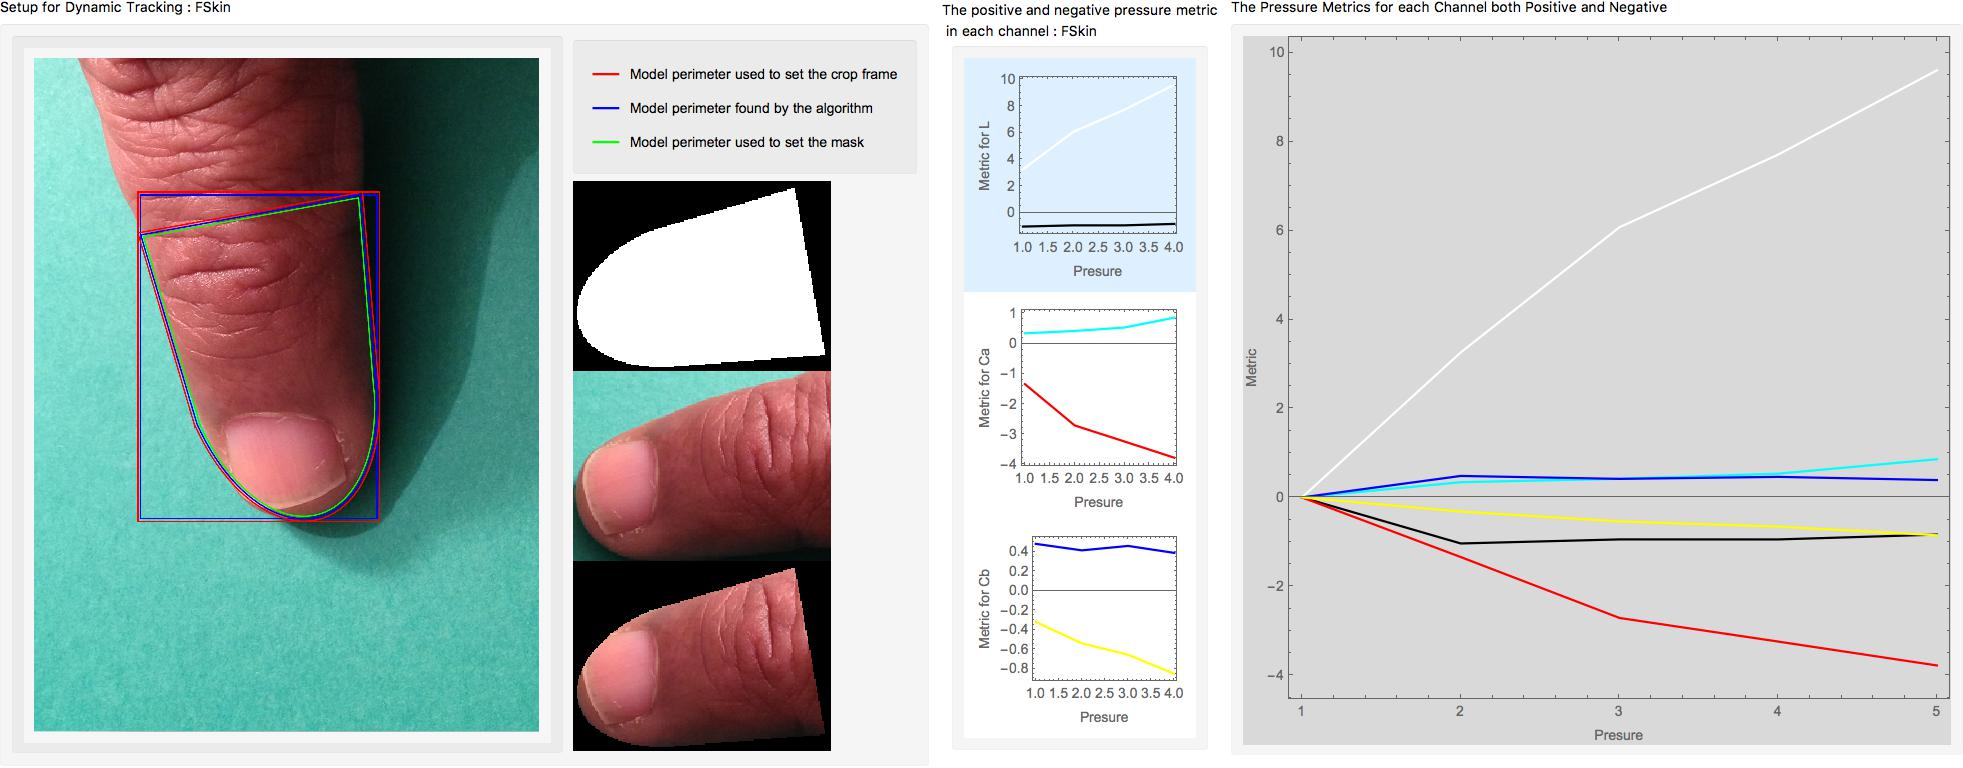
\includegraphics[width=0.820\textwidth]{Chapter4/Figs/Final_Fig_Misc_FSkin.jpg}
        \caption{The resulting sequence of images from the ICWaS algorithm followed by the differences. The metric is the result of summing the positive and negative changes separately and dividing by the number of pixels. Finally the initial image of the sequence is shown with the model outline, the slightly larger model used to set the crop frame and the slightly smaller model used for setting the mask.}\label{fig:ICWaSResultFSkin}
\end{figure}


\begin{figure}[h!]
  \centering
    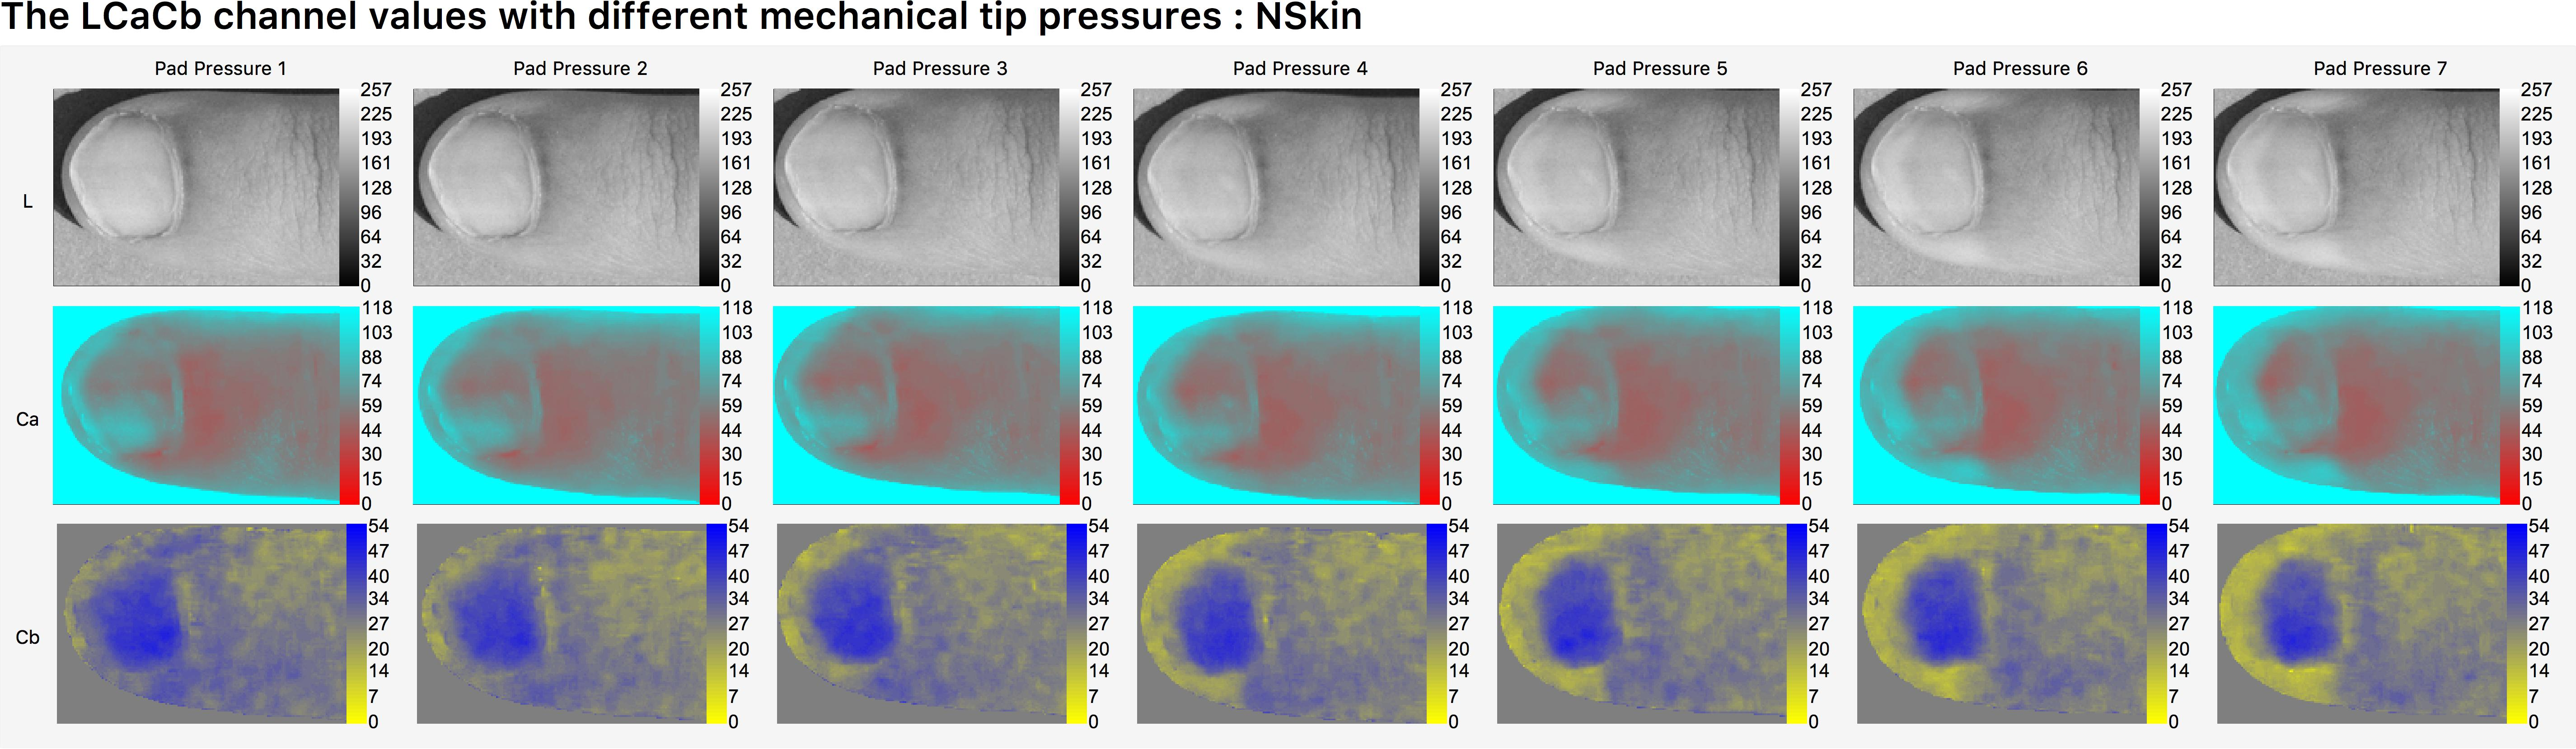
\includegraphics[width=1.00\textwidth]{Chapter4/Figs/Final_Fig_Channels_NSkin.jpg}
    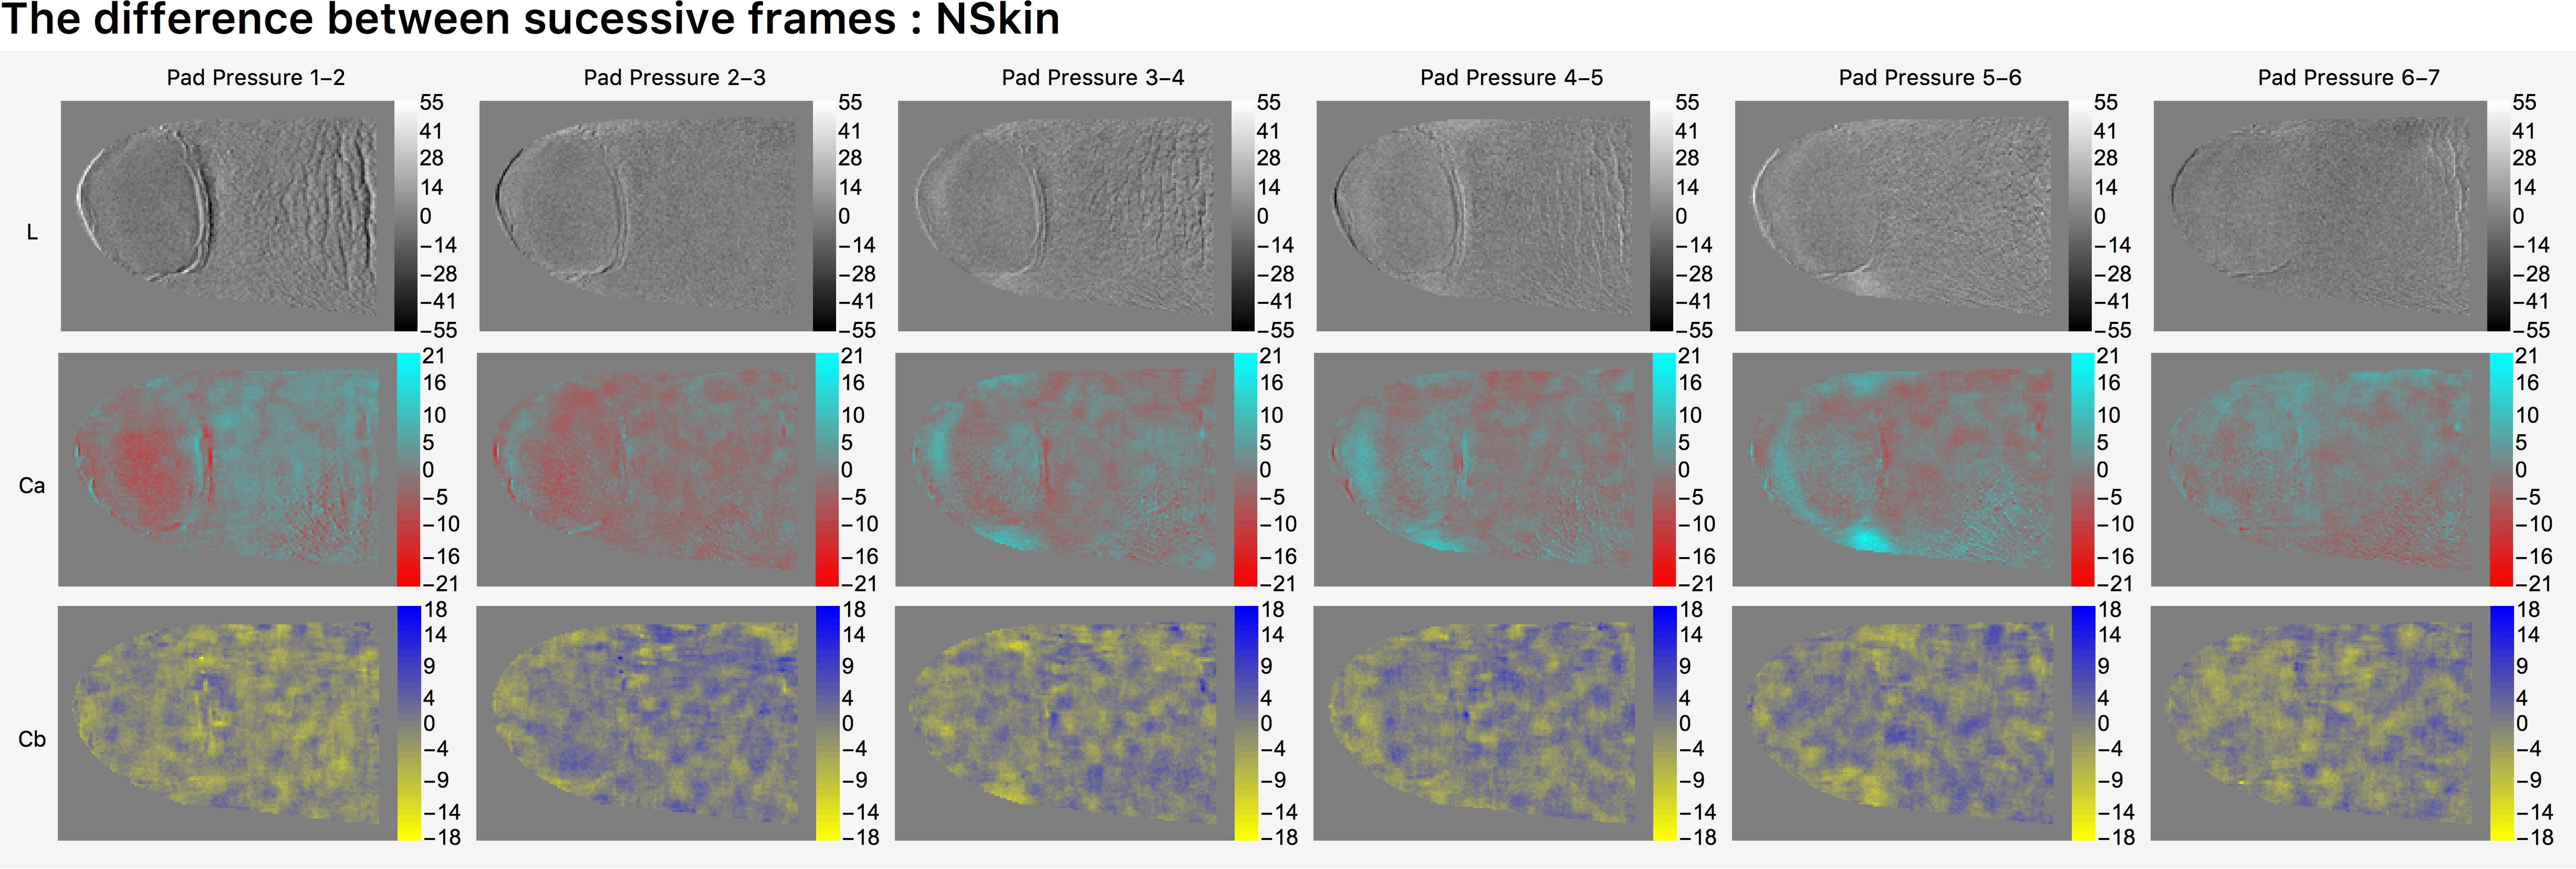
\includegraphics[width=0.86\textwidth]{Chapter4/Figs/Final_Fig_Difference_NSkin.jpg}
    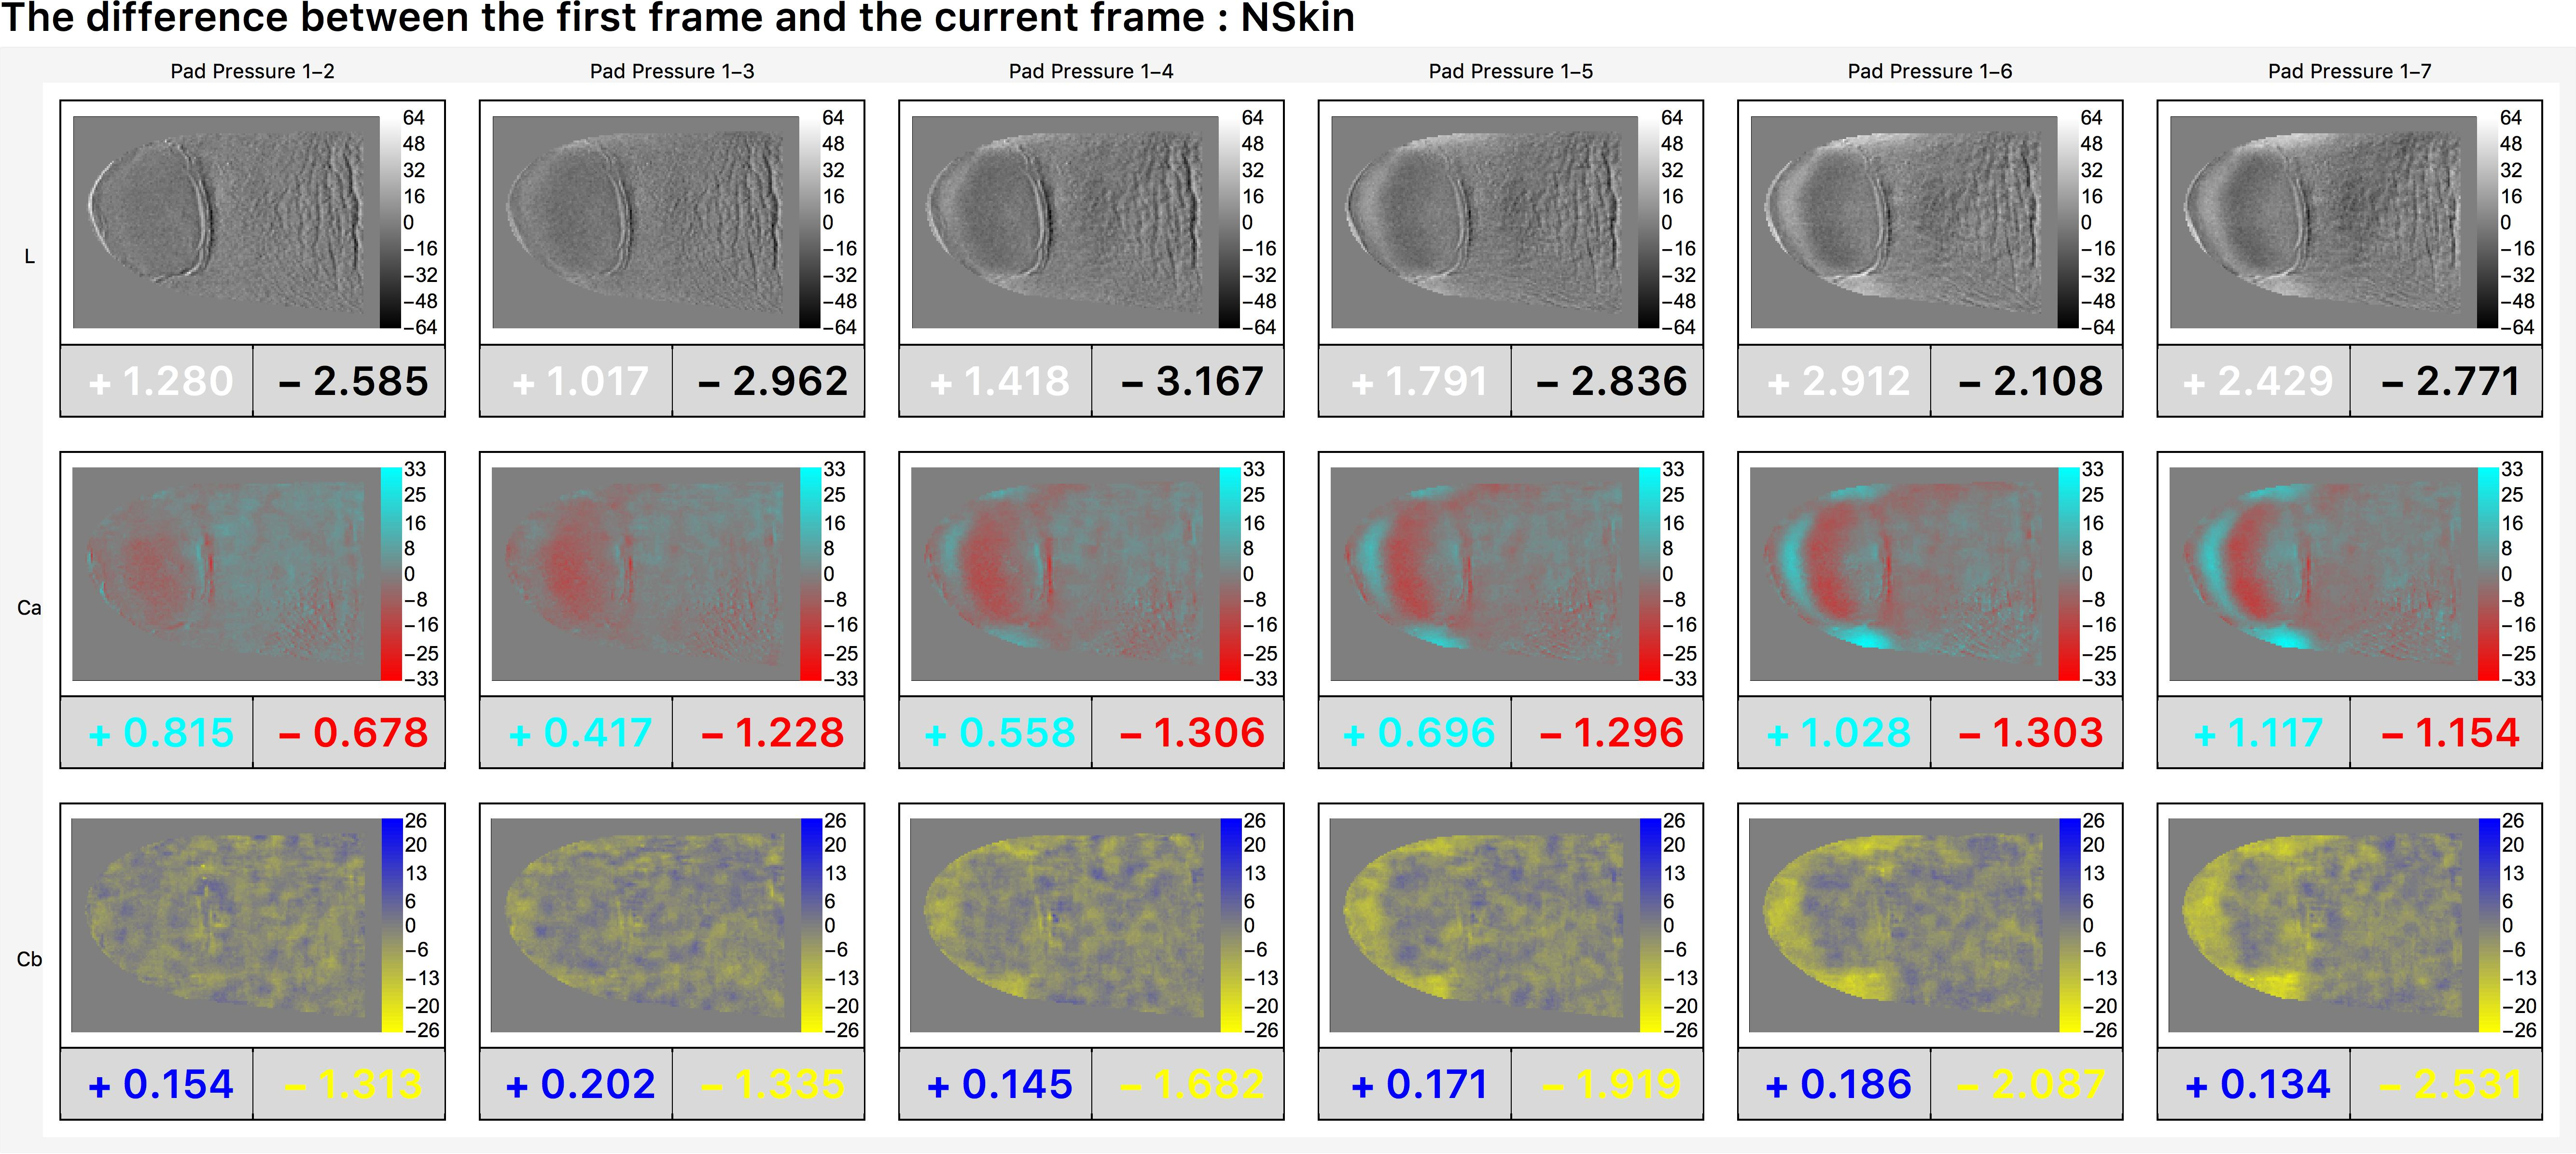
\includegraphics[width=0.86\textwidth]{Chapter4/Figs/Final_Fig_Total_Difference_NSkin.jpg}
    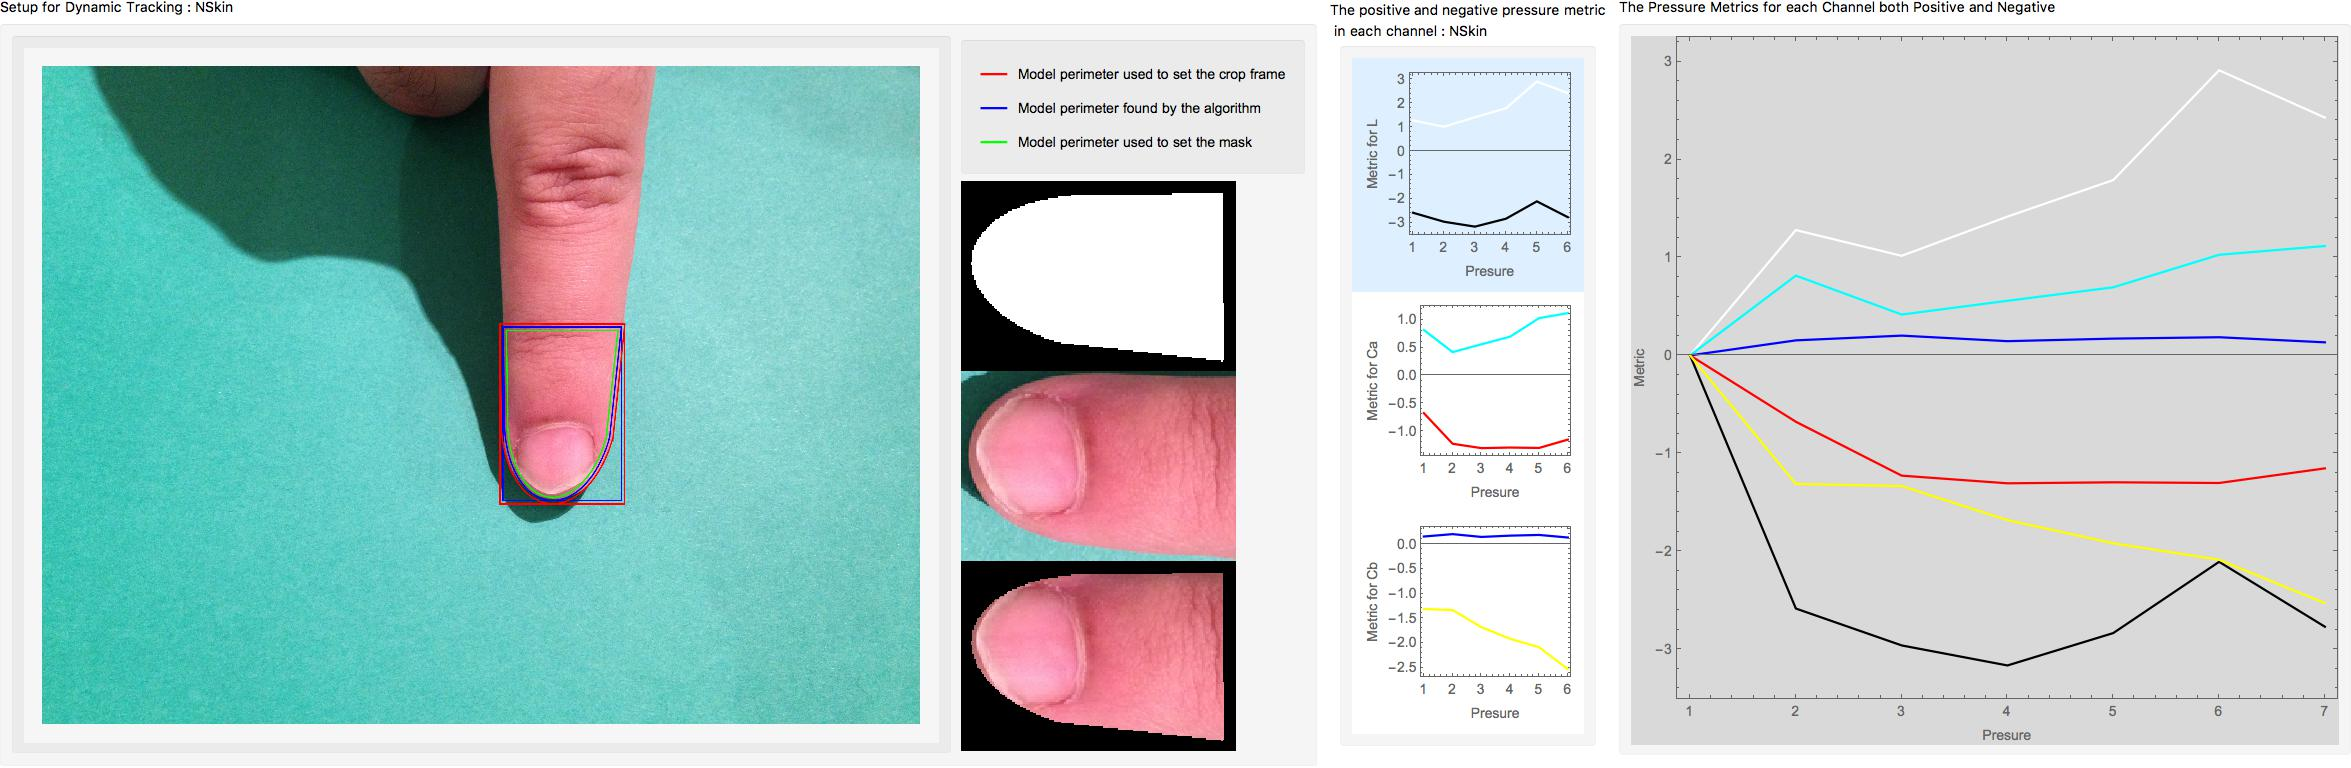
\includegraphics[width=1.00\textwidth]{Chapter4/Figs/Final_Fig_Misc_NSkin.jpg}
        \caption{The resulting sequence of images from the ICWaS algorithm followed by the differences. The metric is the result of summing the positive and negative changes separately and dividing by the number of pixels. Finally the initial image of the sequence is shown with the model outline, the slightly larger model used to set the crop frame and the slightly smaller model used for setting the mask.}\label{fig:ICWaSResultNSkin}
\end{figure}

We assume that the digit's movement will not take it outside of the bounding box set up in the initialization step (section \ref{sec:ICWaSSetup}), so we capture the tip image from the video feed. The RGB tip image is converted to the skin color space, then the grayscale channel image is used to align with the previous captured frame; if this is the first pass through the loop, this is the image captured in the initialization. The frame alignment metric is masked using the binary rastered model image generated in the initialization.

The image alignment pixel shift updates the change in the model position since the first frame. If the change in the model position since the first frame is greater than the ICWaS threshold, then the control passes back to the Smooth Motion routine. The current frame is aligned with the previous frame and the difference is found between the pixel values in the chromatic channels; this is the blood flow (Figures  \ref{fig:ICWaSResultJSkin}, \ref{fig:ICWaSResultFSkin} \& \ref{fig:ICWaSResultNSkin}). These steps are repeated until the change in the model position since the first frame causes the routine to transfer control back to the Smooth Motion routine.

\clearpage

\section{Putting it All Together}\label{sec:PuttingItAllTogether}
So far, we have said little about the app itself; the app associated with this project is designed to demonstrate how the fast color space transform developed in Chapter 2 can be used in conjunction with the simple shape detection routines developed in this chapter to create a simple fingertip mechanical-stress detector using an iPhone.

It is considered good practice when developing an iPhone app to split the code into three parts: the model, which handles all the computation; the view, which handles display and interprets user gestures; and the controller, which is the intermediary, essentially handling the control flow of the user interface. Each can be considered to be running in its own thread, and the Objective-C language handles the interaction between these threads. The recommended division of the control assigns each step in the program as indicated in Figure \ref{fig:FingerpressUI}. 

\begin{figure}[h!]
  \centering
    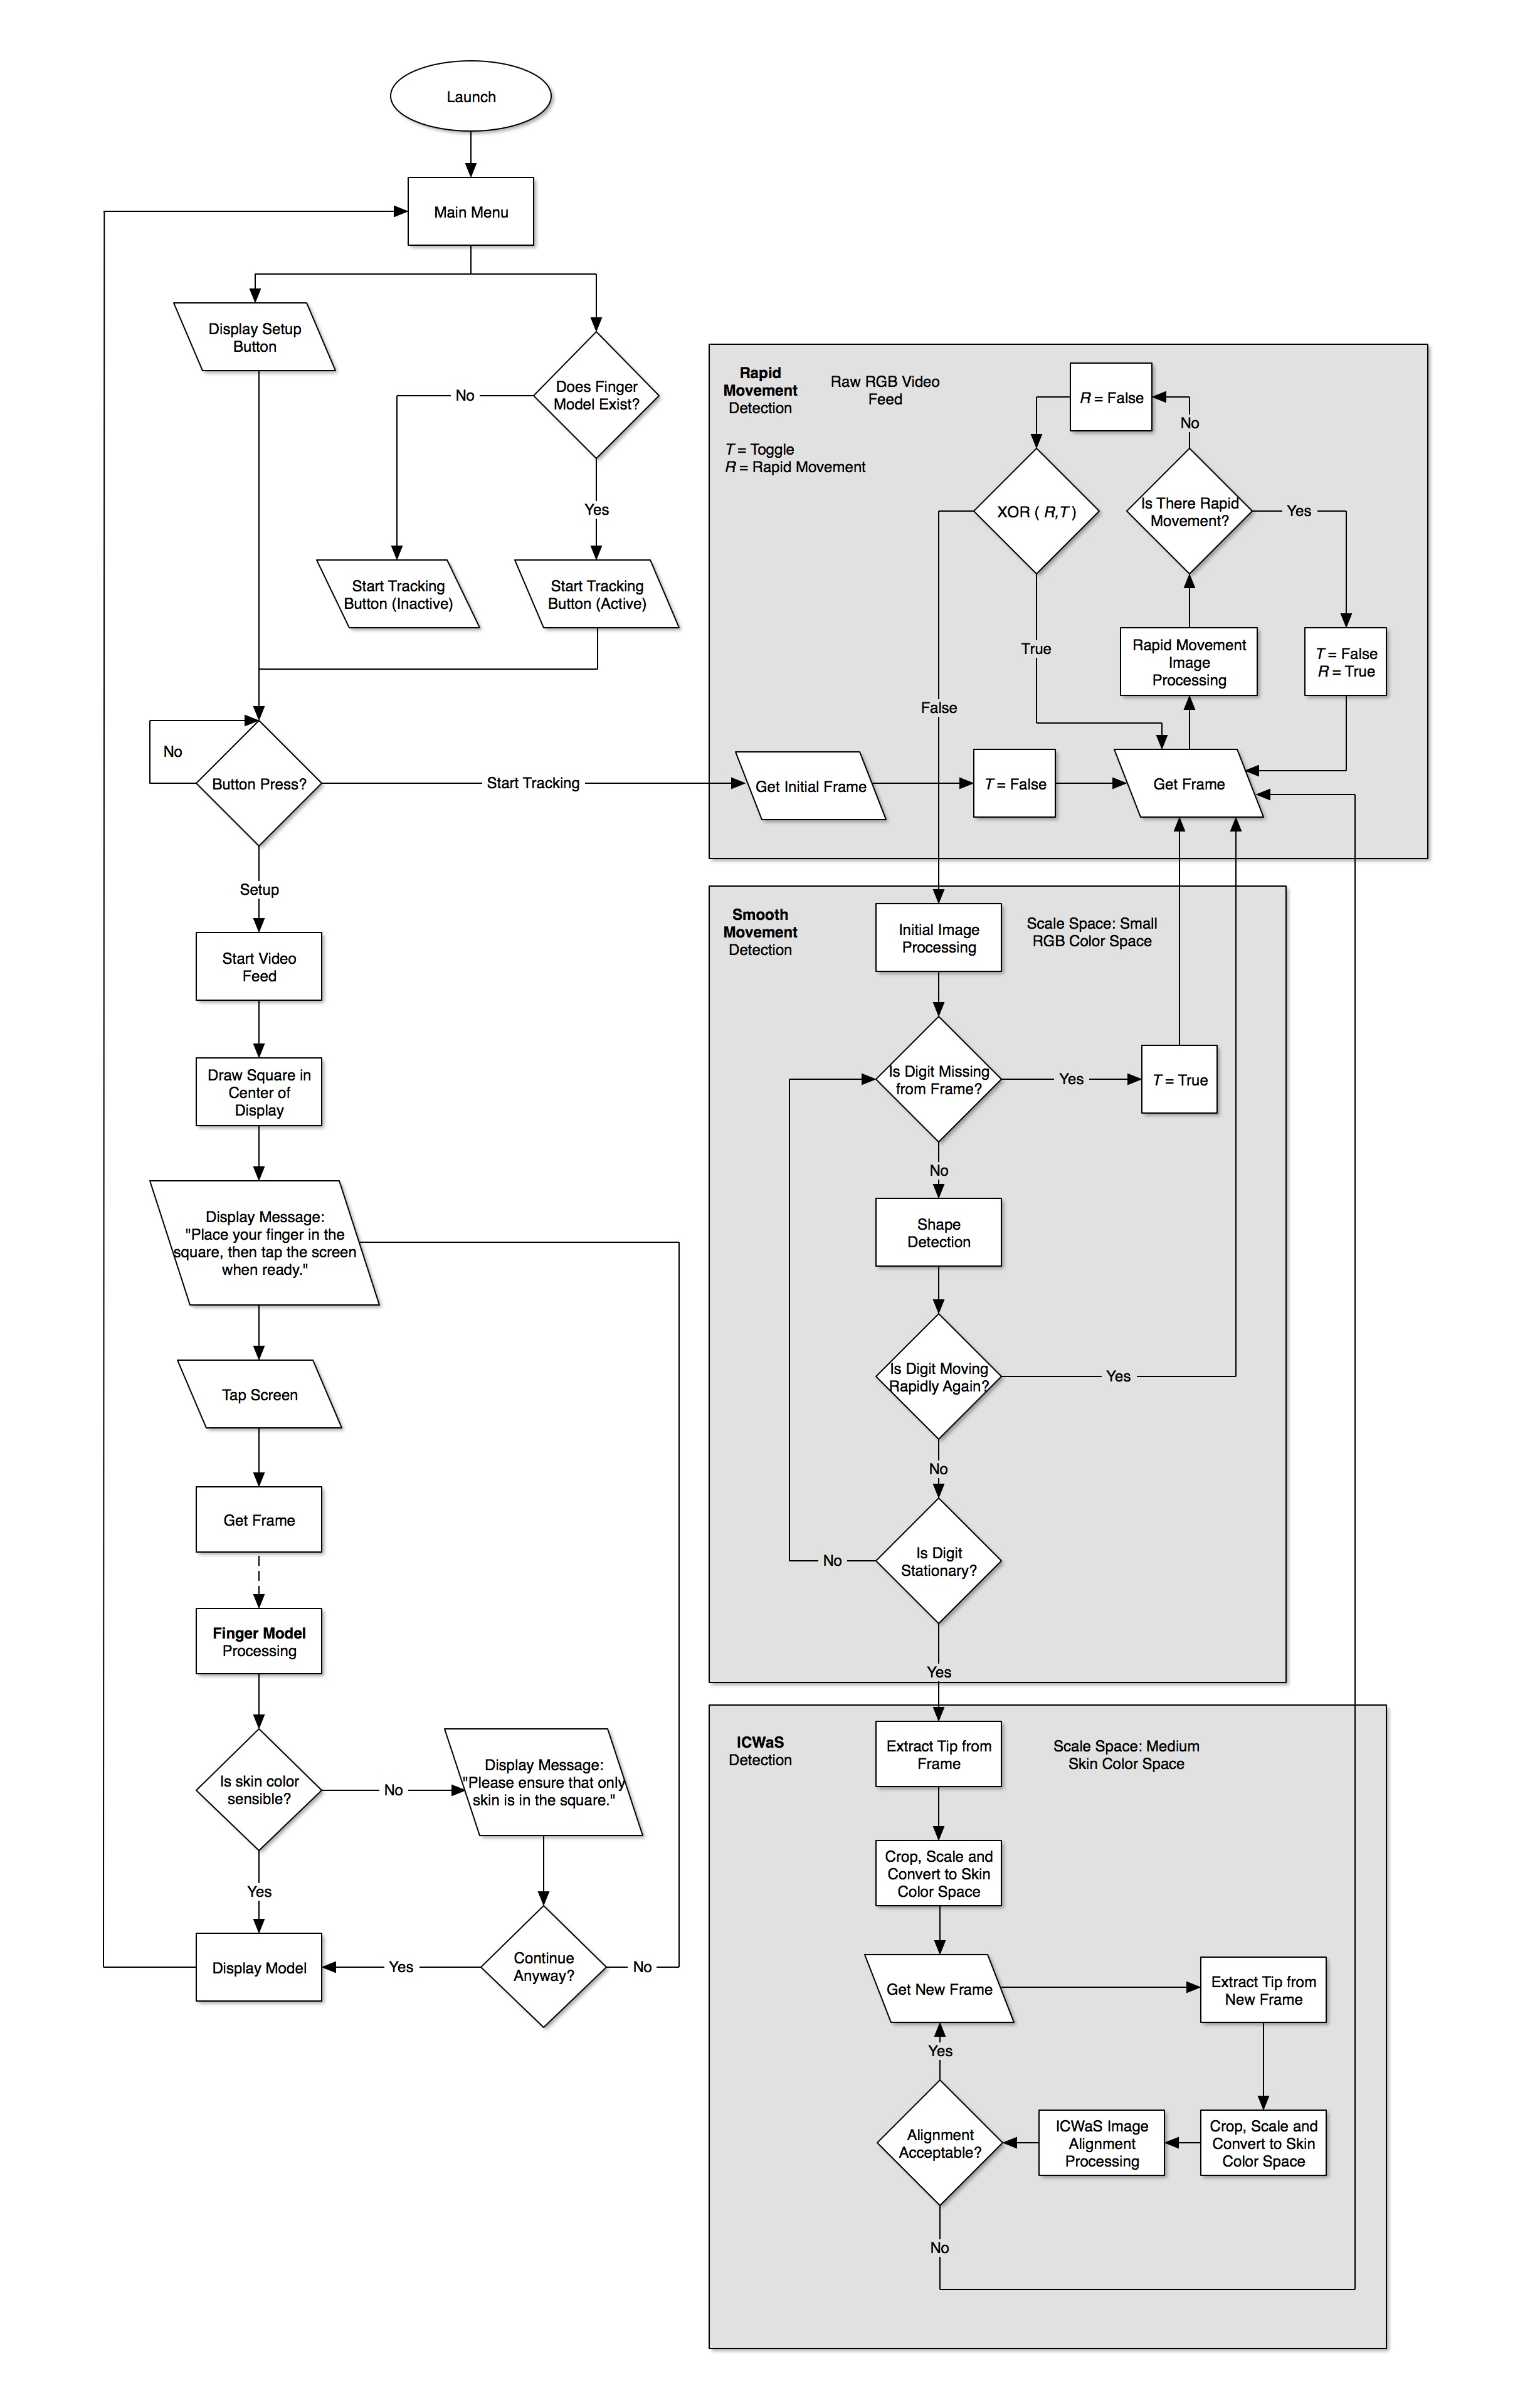
\includegraphics[width=0.97\textwidth]{Chapter4/Figs/Fingerpress_UI.jpg}
    \caption{Fingerpress UI flowchart}\label{fig:FingerpressUI}
\end{figure}

The chart accurately presents the logical flow and recommended assignment of the program elements. However, the chart fails to address how the model, controller and view are each running in their own threads, and so control never actually passes from the model to the controller, or vice versa. So, in the MVC structure, the model and the view may only message the controller to indicate that an event has happened. For instance, when processing a video stream, if every time the dynamic tracking part of the model required a new image, a request message must be sent to the controller, then it would need to wait for the controller to get the image from the video stream and send it to the model, i.e. the model would often be waiting for the controller to respond. For this reason, in practice, the model uses OpenCV's video stream handling capabilities to get an image directly from the video stream.

\begin{figure}[h!]
  \centering
    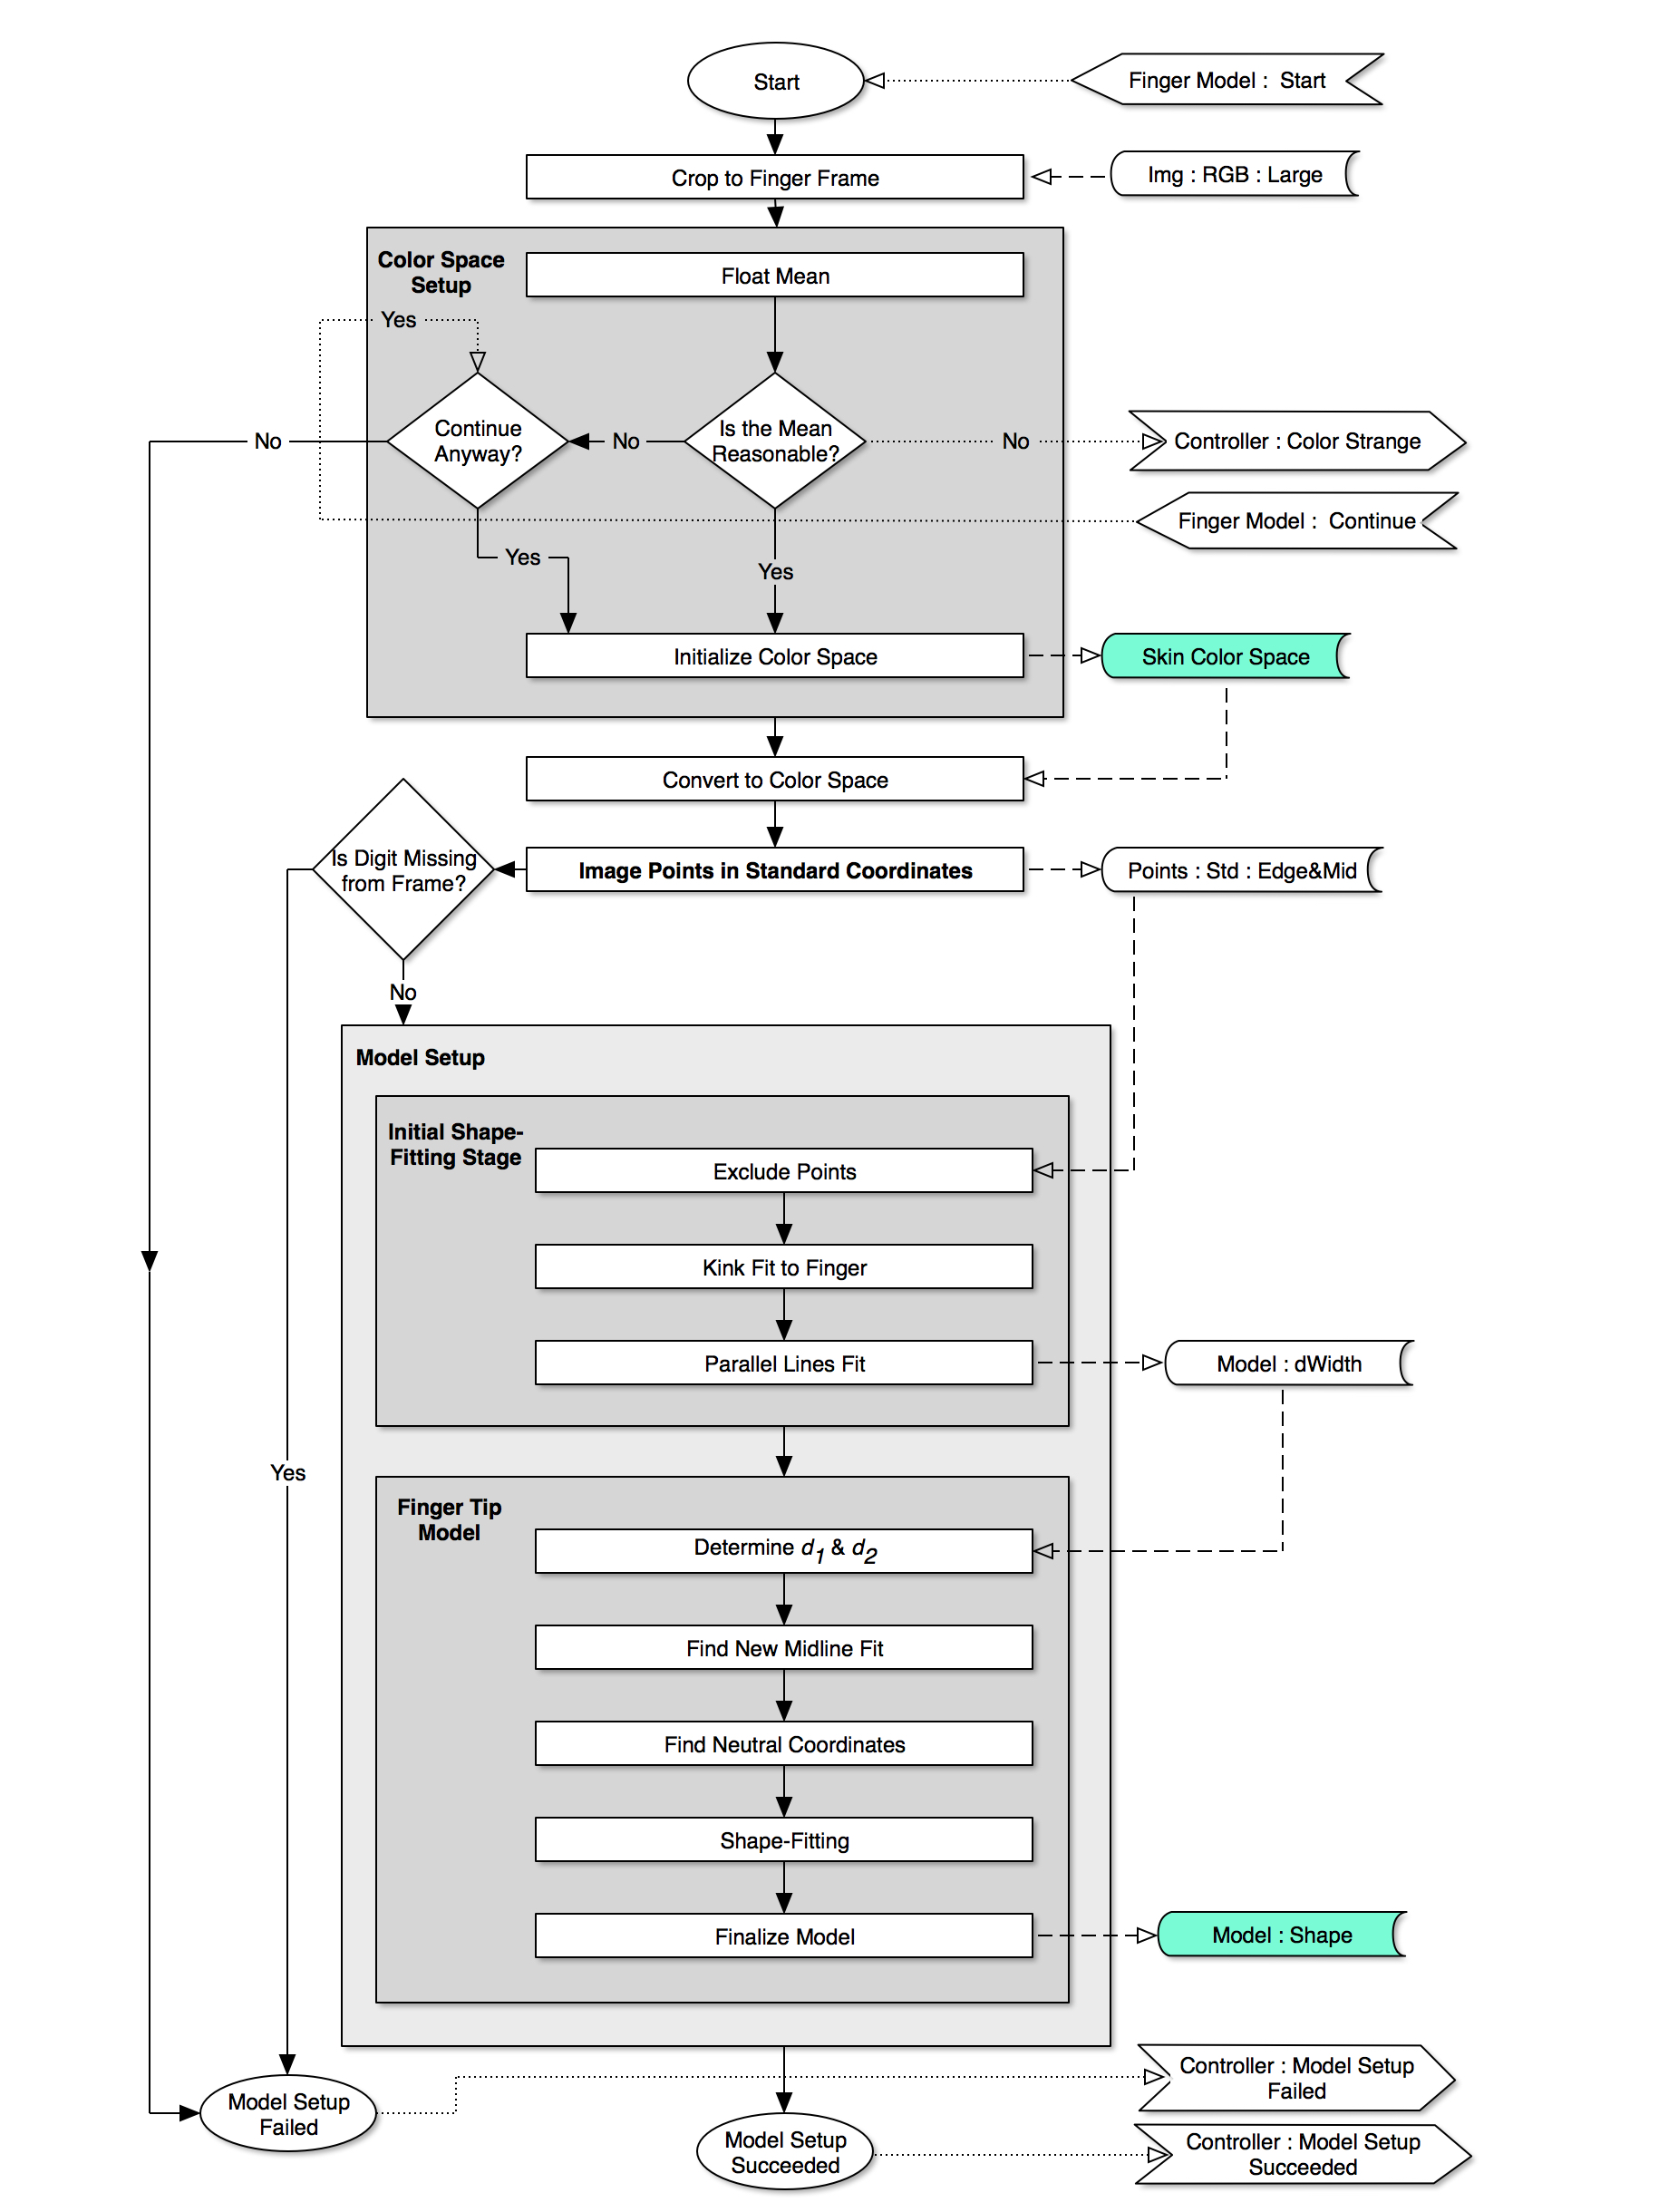
\includegraphics[width=0.95\textwidth]{Chapter4/Figs/Fingerpress_Finger_Model.jpg}
    \caption{Finger model flowchart}\label{fig:FingerpressFingerModel}
\end{figure}

\begin{figure}[h!]
  \centering
    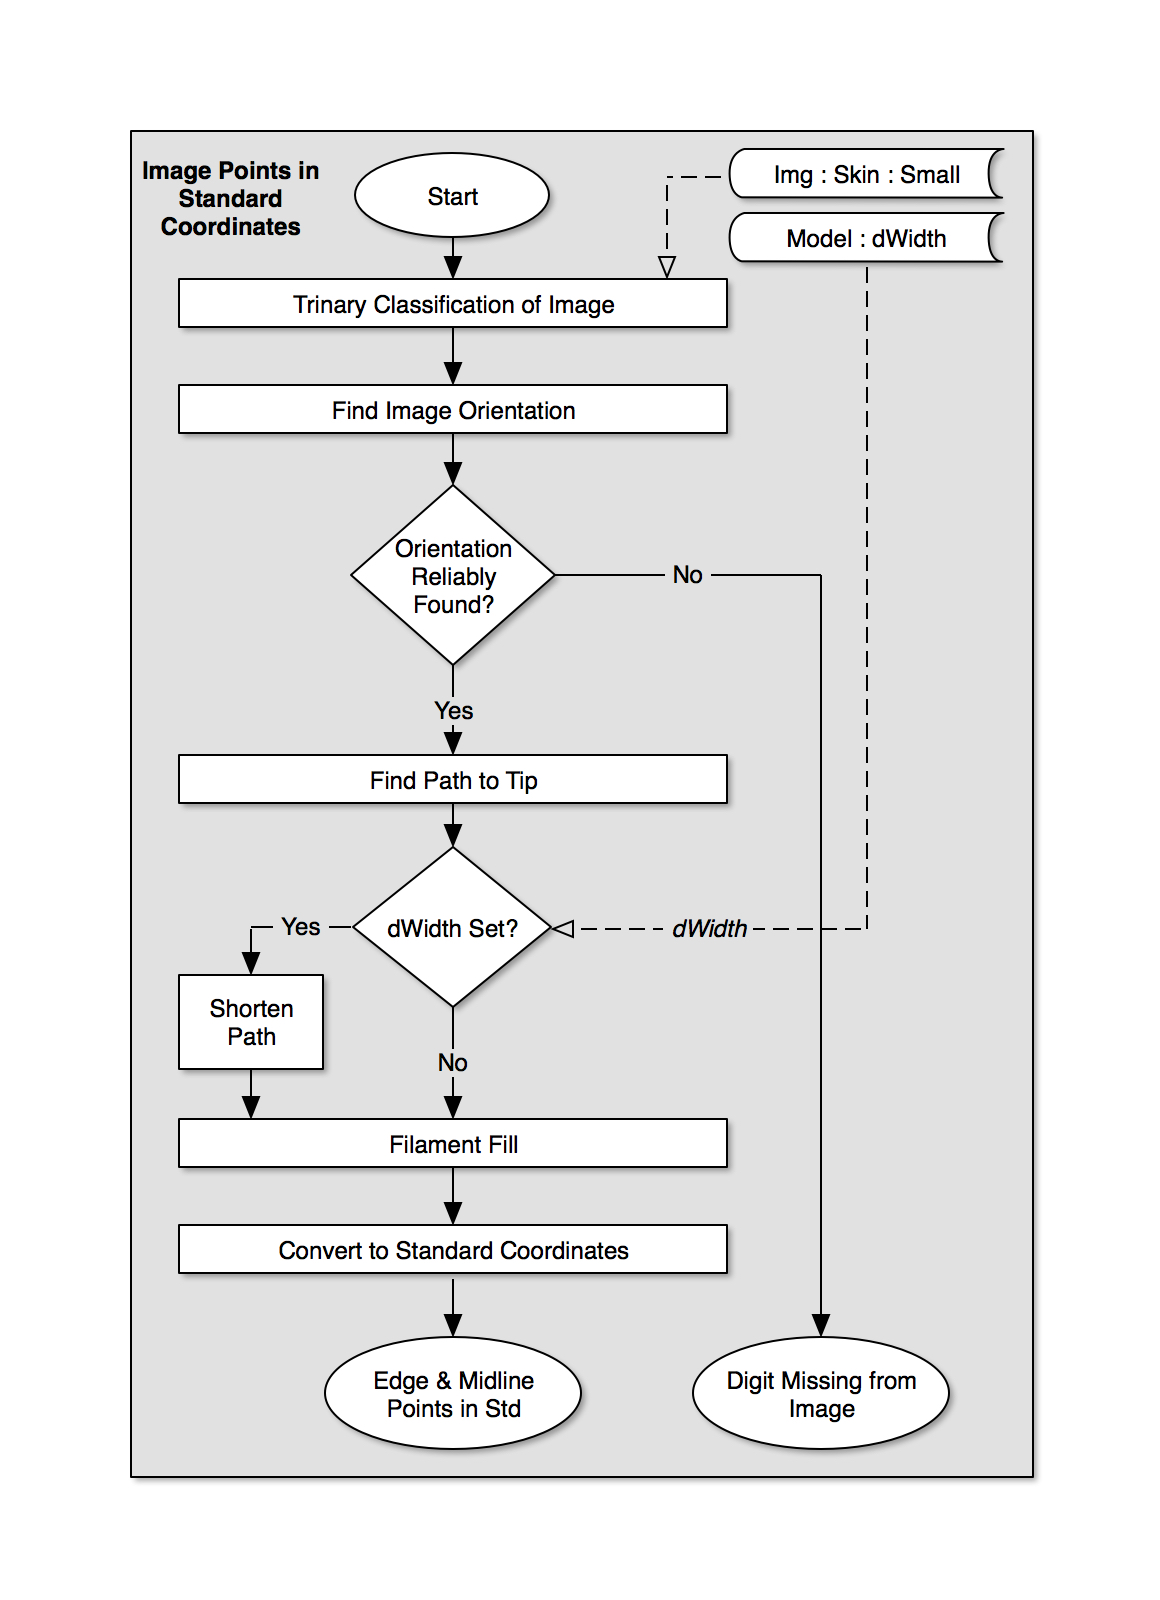
\includegraphics[width=0.49\textwidth]{Chapter4/Figs/Fingerpress_Std_Coordinates.jpg}
    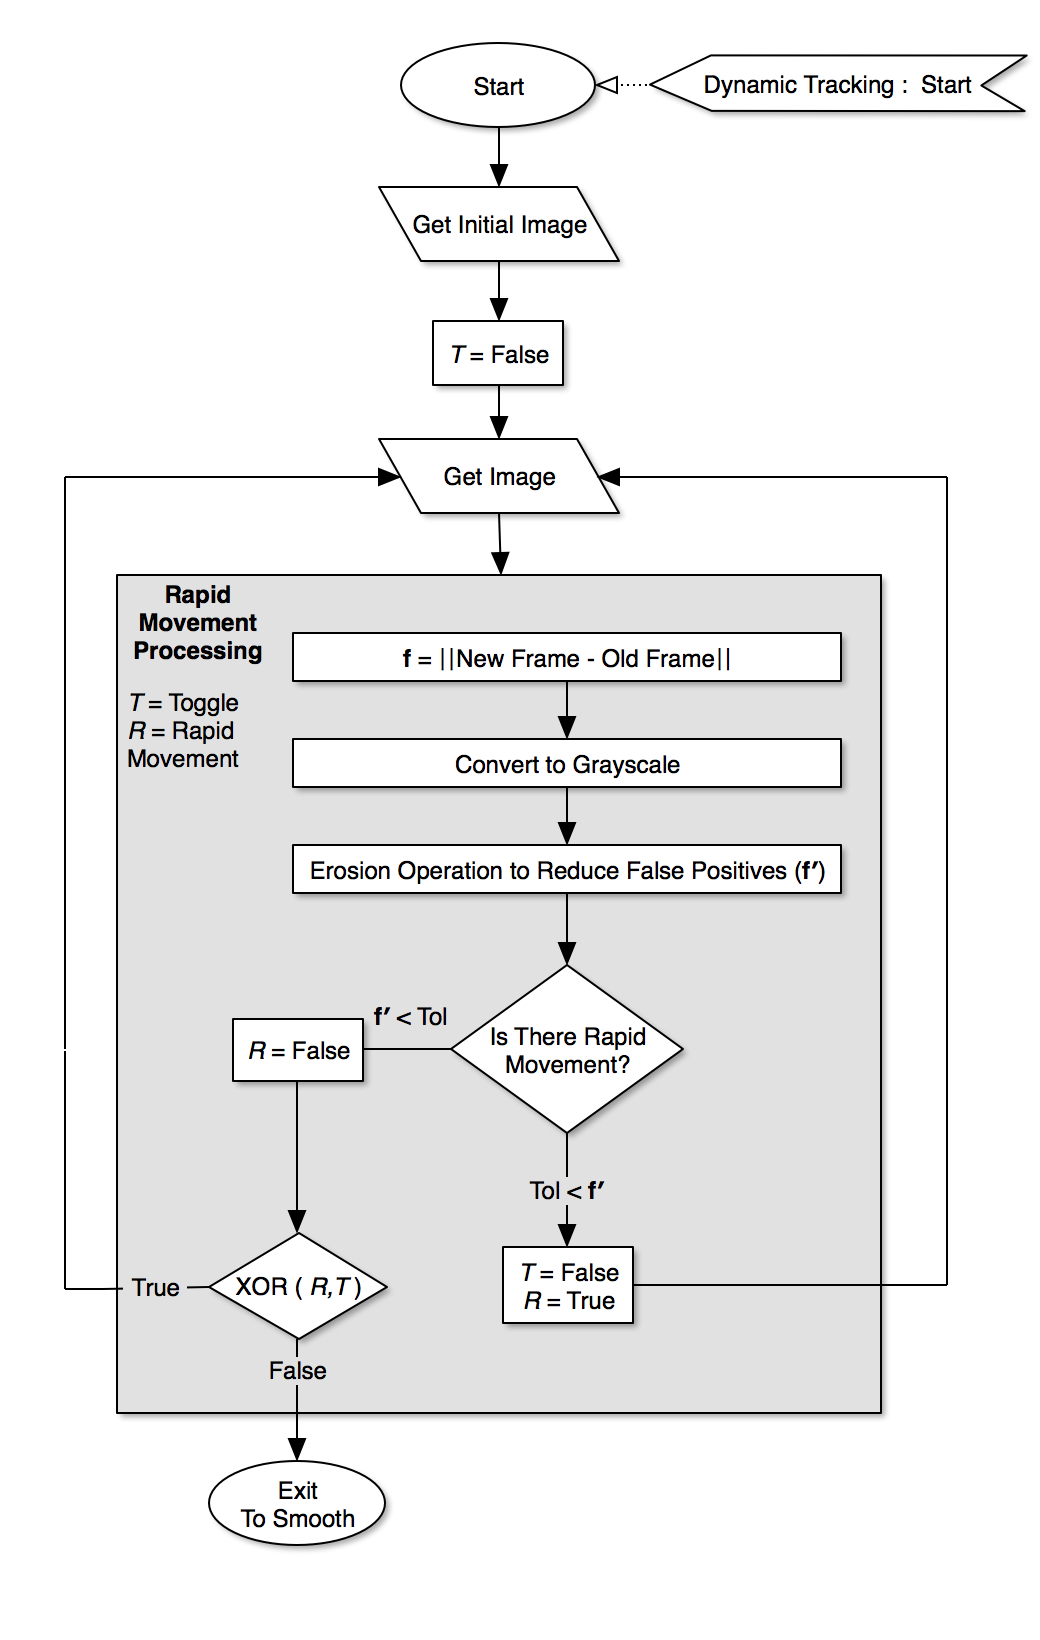
\includegraphics[width=0.49\textwidth]{Chapter4/Figs/Fingerpress_Rapid_Movement.jpg}
    \caption{Flowcharts for finding image points in standard coordinates (left), and rapid motion detection.}\label{fig:FingerpressStdCoordinates&RapidMovement}
\end{figure}

\begin{figure}[h!]
  \centering
    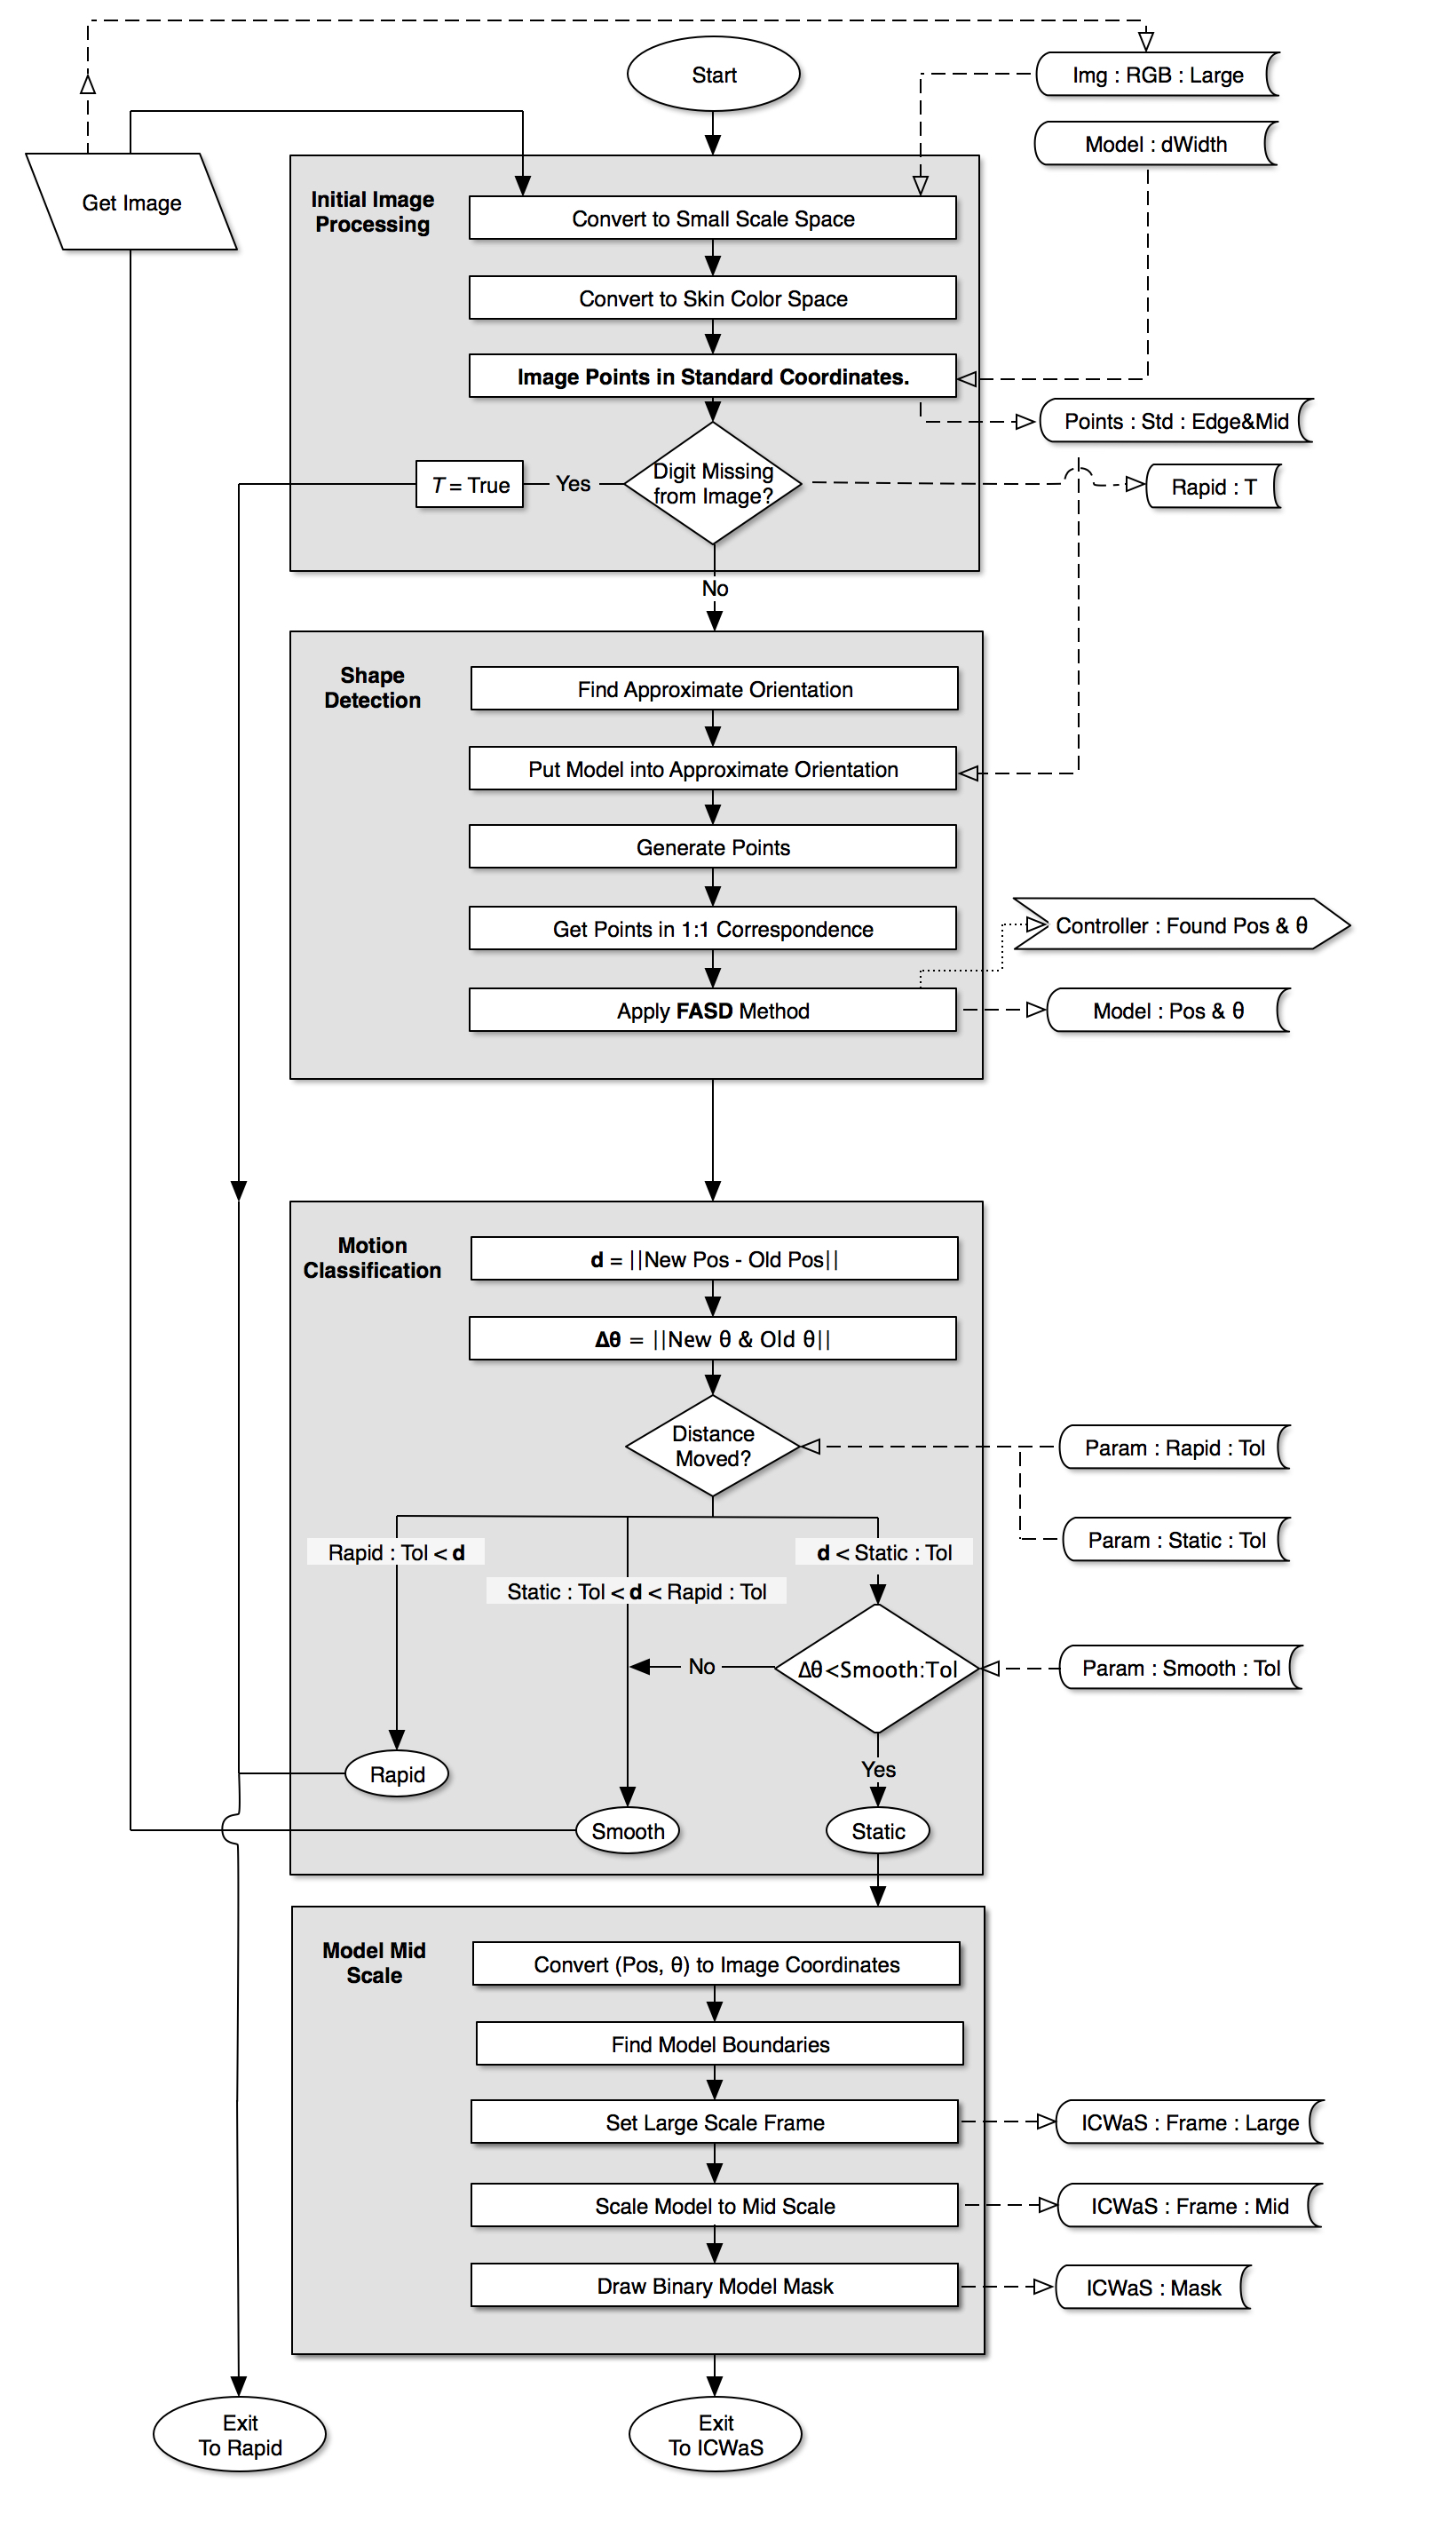
\includegraphics[width=0.90\textwidth]{Chapter4/Figs/Fingerpress_Smooth_Movement.jpg}
    \caption{Smooth movement flowchart}\label{fig:FingerpressSmoothMovement}
\end{figure}

\begin{figure}[h!]
  \centering
    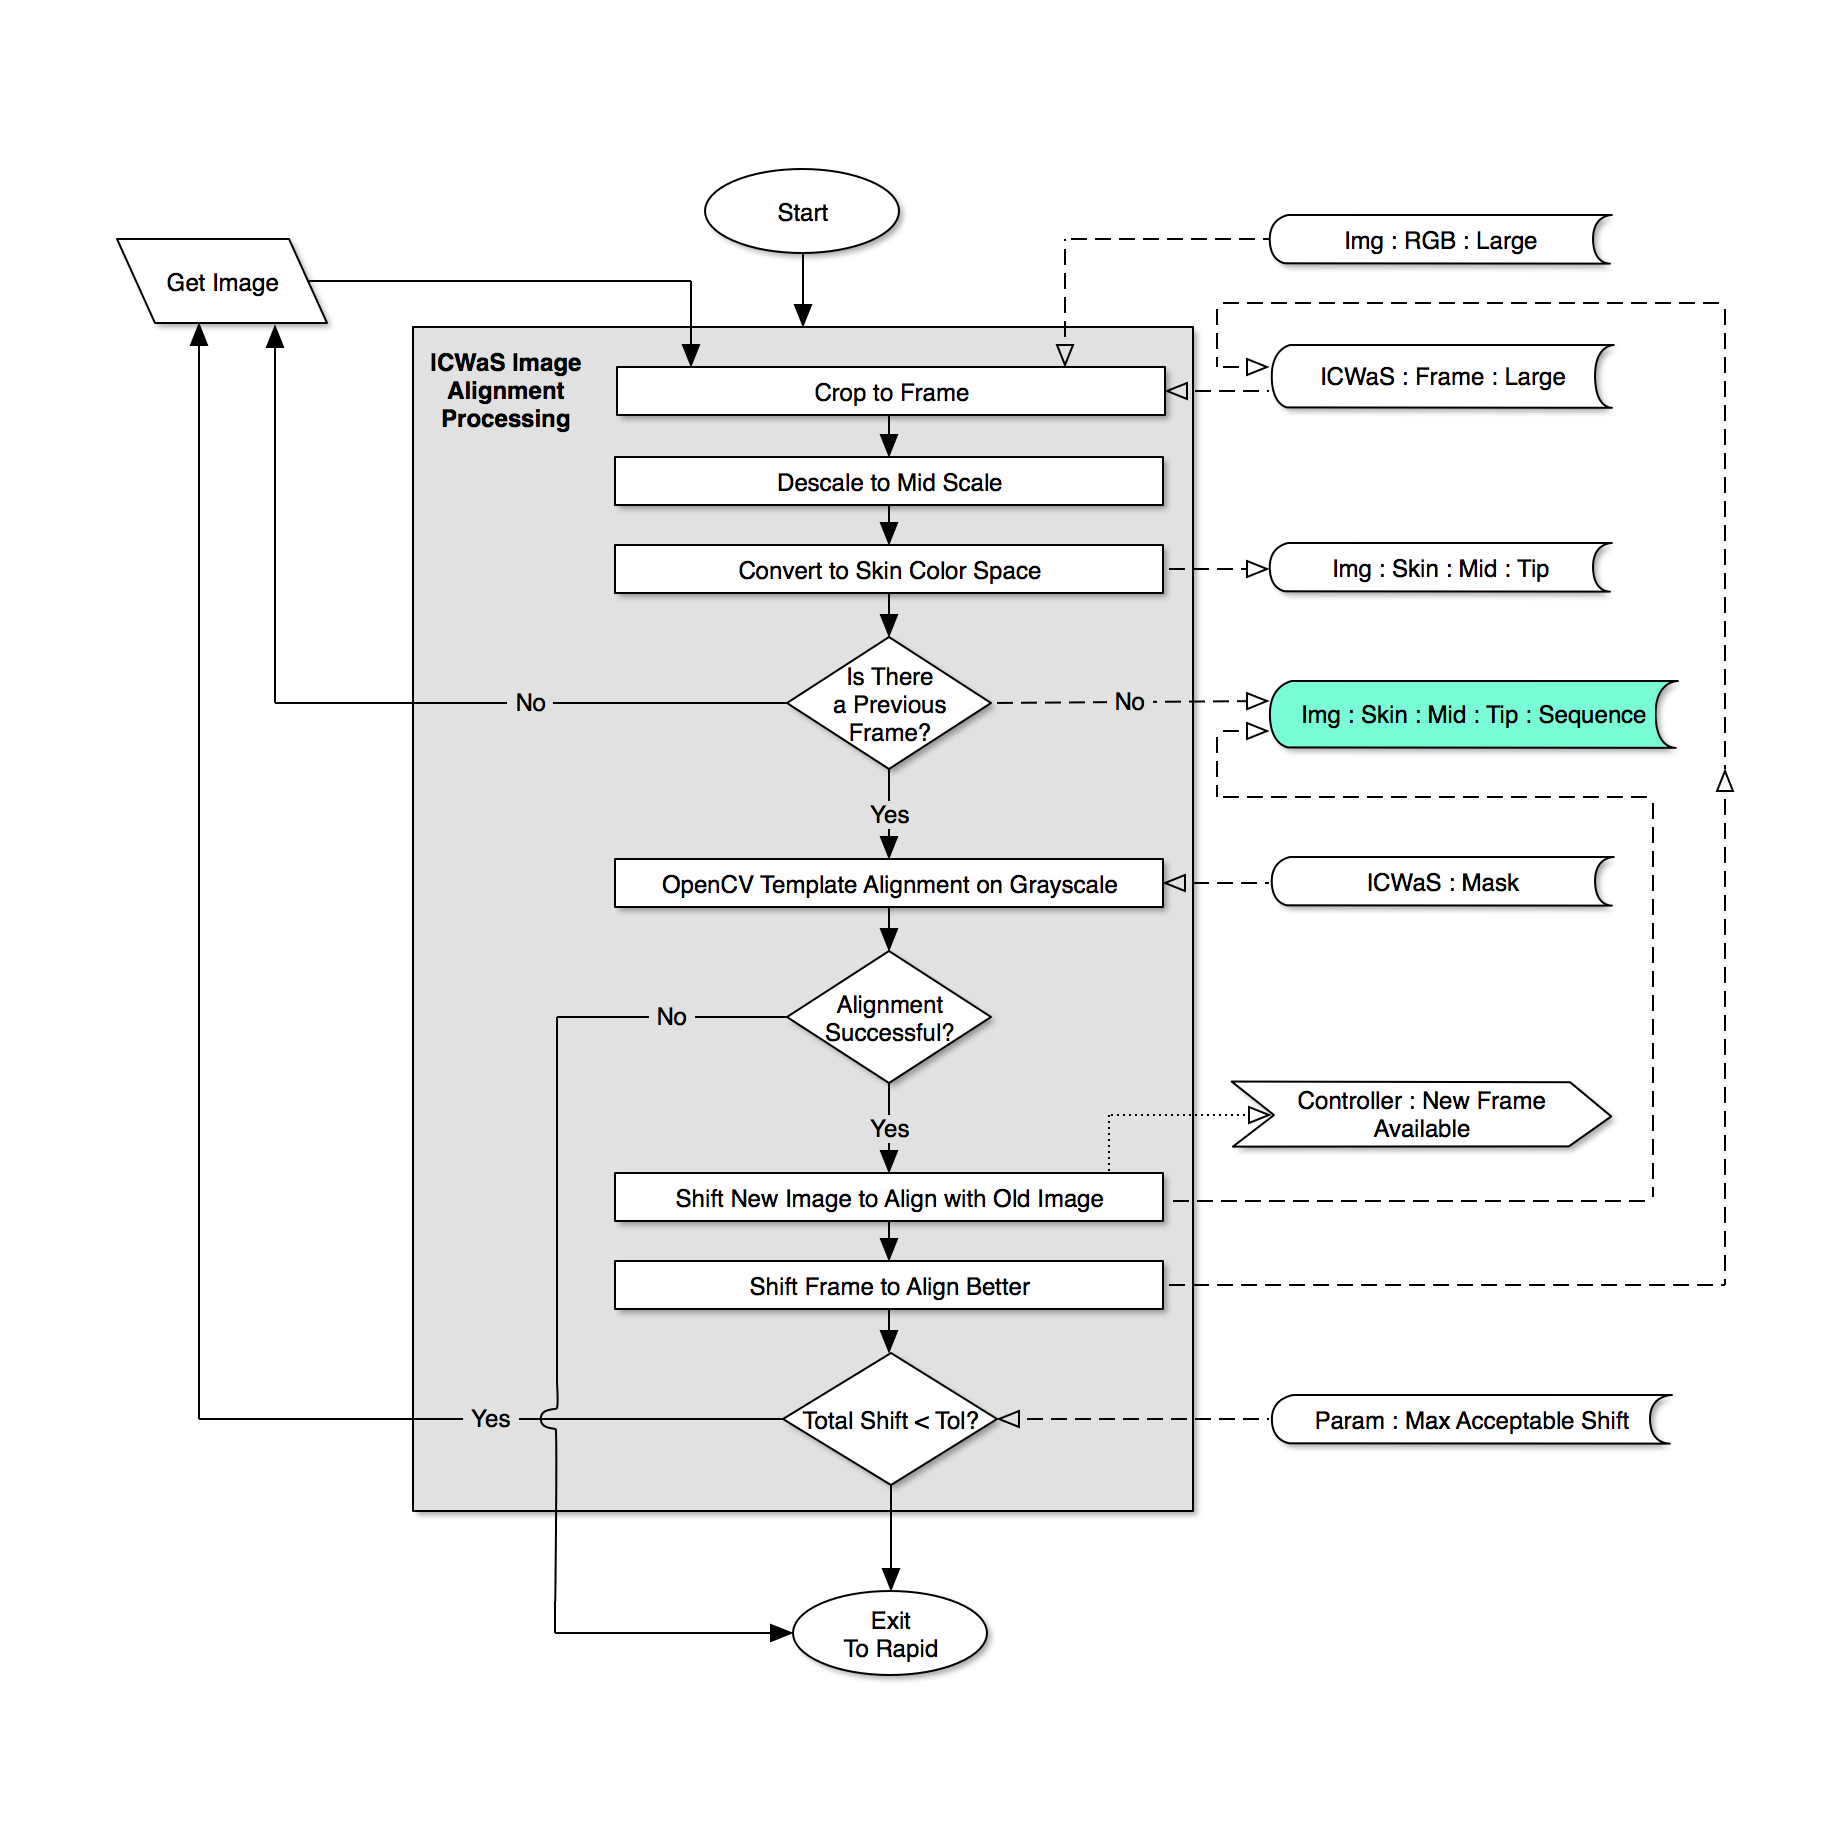
\includegraphics[width=0.95\textwidth]{Chapter4/Figs/Fingerpress_ICWaS.jpg}
    \caption{ICWaS flowchart}\label{fig:FingerpressICWaS}
\end{figure}

The charts in Figures \ref{fig:FingerpressFingerModel}, \ref{fig:FingerpressStdCoordinates&RapidMovement}, \ref{fig:FingerpressSmoothMovement} and \ref{fig:FingerpressICWaS} more accurately depict the actual implementation of the model by showing the data flow to the elements of the model which are accessible to the controller. 

